\documentclass[11pt]{article}
\PassOptionsToPackage{numbers,sort&compress}{natbib}
\usepackage[eandd]{neurips_2026}

\usepackage[utf8]{inputenc}
\usepackage[T1]{fontenc}
\usepackage{hyperref}
\usepackage{url}
\usepackage{booktabs}
\usepackage{amsfonts}
\usepackage{amssymb}
\usepackage{amsmath}
\usepackage{nicefrac}
\usepackage{microtype}
\usepackage{graphicx}
\usepackage{xcolor}
\usepackage{multirow}
\usepackage{makecell}
\usepackage{enumitem}
\usepackage{subcaption}
\usepackage{algorithm}
\usepackage{algorithmic}

\title{LADDER: LLM Agent Diagnostic of Domain-level Estimation Reliability}

\author{
  Anonymous Authors
}

\begin{document}

\maketitle

%==============================================================================
% ABSTRACT
%==============================================================================
\begin{abstract}
Users learn where each LLM agent is reliable; the agent itself does not. We ask a single mechanistic question: at which sub-capability does this self-modeling break down? Three candidates---H1 output channel, H2 prior metacognition, H3 noise-robust online inference---are conflated by standard benchmarks. We build \textbf{LADDER}, a diagnostic benchmark whose five-level oracle ladder (L0 raw confidence $\to$ L4 full-statistic oracle) lets each adjacent comparison rule out one candidate, scored with \textbf{Capability Boundary Fidelity (CBF)}, a per-domain metric distinct from per-query calibration (ECE). The ladder yields a clean localization across 19 models. H1 is ruled out (GT-SelfStats CBF $\geq 0.99$ on every model); H2 is partial and family-split rather than the bottleneck (GPT models reach 0.795--0.859 zero-shot, while the three Claude-4-6/4-7 models fall below NoMemory). H3 is the locus: first-order single-rater learners cluster near NoMemory, while explicit \emph{second-order} estimators (asymmetric Dawid--Skene, GLAD) substantially exceed the L1 prior, with GLAD winning on all nine frontier models (binomial sign-test $p=0.002$). The pattern replicates across task families (13/19 sign-flip rate on extension tasks), implying that per-task boundary modeling is also needed. We name this failure mode \textbf{Self-Boundary Collapse} and identify noise-robust second-order online inference as the central remaining challenge. We release the ladder, CBF, cross-family user simulator, and trace dataset as benchmark infrastructure.
\end{abstract}

%==============================================================================
% 1  INTRODUCTION
%==============================================================================
\section{Introduction}
\label{sec:intro}



LLM agents are increasingly used in long-horizon, multi-turn settings, including customer service, coding, research, and tool use. Over time, users develop an empirical sense of where an agent is reliable. The agent, however, typically retains no comparable self-model: each session begins without prior calibration and ends by discarding its own evidence. This asymmetry is well documented, but the underlying \emph{capability gap} remains poorly localized. In particular, we do not yet know \emph{where}, mechanistically, agent self-modeling fails.

We distinguish three possible bottlenecks. Under H1, the output channel is the limiting component: the model cannot format and emit numerical per-domain statistics. Under H2, the model lacks an accurate prior over its own per-domain abilities, so any useful self-assessment must be \emph{learned} through interaction. Under H3, the model can state reasonable priors but cannot update them reliably from \emph{noisy} implicit user feedback. These hypotheses imply different intervention targets. H1 suggests fine-tuning for numerical reporting; H2 points to pre-training-time metacognitive curricula; H3 calls for noise-robust online estimation. Existing work on agent self-knowledge \citep{barkan2026capable, hu2026memoryagent}, calibration~\citep{kadavath2022language, guo2017calibration, xiong2024can}, and memory systems~\citep{packer2023memgpt, mem02025, tan2025rmm, xu2025amem, li2025memos} measures important symptoms but does not isolate which of these bottlenecks is responsible. We refer to the resulting failure mode, in which LLM agents repeatedly receive feedback yet fail to convert it into a stable domain-level self-model, as \textbf{Self-Boundary Collapse}. Our central question is where this failure appears on the H1/H2/H3 ladder.

We study this question with LADDER. The benchmark is organized around an oracle-bracketed \emph{five-level baseline ladder}: L0 raw confidence (NoMemory), L1 zero-shot per-domain prior, L2 noisy-feedback learners (LLM-self-assessment, classical recalibration, EM-joint, second-order Dawid--Skene/GLAD), L3 binary-label oracle, and L4 full-statistic oracle. Adjacent comparisons localize the failure. L4--L3 tests the output channel (H1), L3--L1 tests the prior (H2), and L3--L2 tests online inference from noisy feedback (H3). The protocol pairs each agent with a domain-heterogeneous simulated user, reliable 75\% of the time in-expertise and 46\% out, with cross-family routing to mitigate a dual-role bias that we quantify in \S\ref{sec:bottleneck}. Sessions last 50 turns, and the resulting per-domain self-model is evaluated with \textbf{Capability Boundary Fidelity (CBF)}, a metric we introduce to complement per-query calibration measures such as ECE.

Across 19 models from 8 families and 60K+ interactions, the ladder gives a clear localization. H1 is ruled out: GT-SelfStats reaches CBF $\geq 0.99$ on every model, showing that the output channel can faithfully emit per-domain statistics when supplied. H2 is real but not the main bottleneck. The zero-shot prior is the strongest non-oracle baseline for GPT models, with CBF 0.795 on GPT-5.4 and 0.859 on GPT-5.5, but it falls below NoMemory on all three Claude-4-6/4-7 models, 0.460--0.482 vs.\ 0.557--0.603; the frontier mean ($n{=}9$) is 0.654. Thus prior self-knowledge exists in some families and is absent in others, but it never reaches the oracle ceiling. The main failure is H3. First-order single-rater learners, including UF-PDC, Platt, HistBin, Bayes, and simple EM-Joint, cluster near NoMemory on the frontier ($n{=}9$ CBF 0.623--0.625), and cannot recover per-domain accuracy from noisy feedback. Explicit \emph{second-order} estimators do substantially better: asymmetric Dawid--Skene reaches a frontier mean of 0.768, and GLAD reaches 0.742. GLAD beats L1 on all nine frontier models, with binomial sign-test $p=0.002$. A remaining L2$\to$L3 gap of roughly 0.23 CBF on the frontier (best L2 DS-asym 0.768 vs.\ OraclePDC 1.000) persists, but it appears tractable rather than fundamental. Figure~\ref{fig:overview} summarizes the protocol, the noisy-feedback channel, and the diagnostic localization in three panels.

\begin{figure*}[t]
\centering
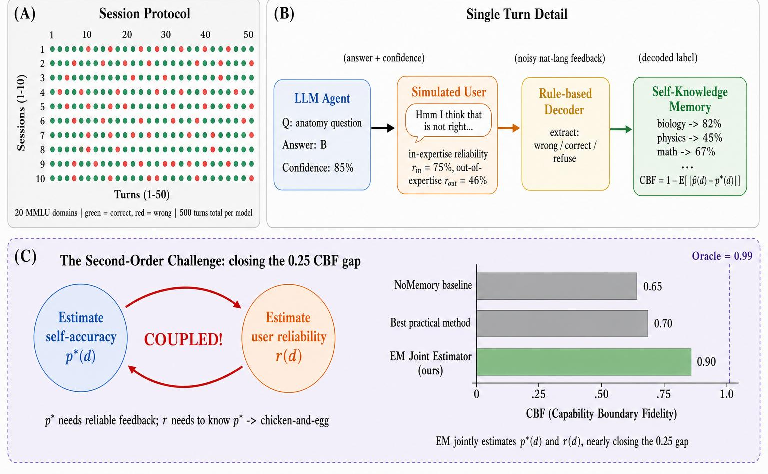
\includegraphics[width=\textwidth]{figures/fig1_overview.pdf}
\caption{\textbf{The L0--L4 oracle ladder localizes where agent self-knowledge fails.} \textbf{(A)}~50 sessions $\times$ 50 turns over 20 MMLU domains (green=correct, red=wrong). \textbf{(B)}~Single turn: agent answers with confidence; a cross-family simulated user gives noisy feedback ($r_{\text{in}}\!\approx\!75\%$, $r_{\text{out}}\!\approx\!46\%$); a decoder extracts the label that updates the per-domain self-model. \textbf{(C)}~The five diagnostic levels with adjacent comparisons isolating H1 (output channel, ruled out at L4--L3), H2 (prior metacognition, family-split at L3--L1), and H3 (noise-robust online inference, the locus at L3--L2).}
\label{fig:overview}
\end{figure*}

\paragraph{Contributions.} (i) A benchmark whose adjacent-level comparisons isolate one sub-capability each, supported by an oracle-bracketed five-baseline ladder; (ii) the per-domain Capability Boundary Fidelity (CBF) metric, distinct from per-query ECE; and (iii) empirical evidence---across 19 models from 8 families and 60K+ noisy-feedback turns---that an H3-class noise-robust online estimator is the central remaining bottleneck for agent self-modeling, with explicit second-order estimators (DS-asym, GLAD) the most promising direction.

%==============================================================================
% 2  RELATED WORK
%==============================================================================
\section{Related Work}
\label{sec:related}

LADDER sits at the intersection of four lines of work---single-shot LLM self-knowledge and calibration benchmarks, multi-step agent overconfidence under clean feedback, multi-turn agent benchmarks that score task completion rather than self-knowledge, and inference-time memory and feedback-learning systems. We position LADDER against each line and summarize the design-axis comparison in Table~\ref{tab:related_axes}; the diagnostic distinction is that LADDER is the only benchmark that combines a noisy domain-dependent feedback channel with an oracle-bracketed accumulation horizon.

\paragraph{LLM self-knowledge and calibration benchmarks.} A growing line of work probes whether LLMs can represent or report their own correctness on a single query. Internal-representation studies show that latent confidence signals exist~\citep{kadavath2022language, jian2025metacognition, binder2025introspection}, while recent benchmarks evaluate metacognition behaviorally and find that frontier models exhibit only partial, context-dependent self-monitoring~\citep{ackerman2026metacognition, liu2025metacognitive_learning}. Table~\ref{tab:related_axes} positions the most closely related benchmarks against LADDER along four design axes: feedback channel, horizon, whether self-knowledge is accumulated, and whether the protocol forces second-order user-reliability inference.

\begin{table}[h]
\centering
\caption{\textbf{Related-benchmark positioning along four design axes.} LADDER is the only benchmark combining a noisy interactive feedback channel, accumulation horizon, and second-order user-reliability inference.}
\label{tab:related_axes}
\vspace{0.3em}
\scriptsize
\setlength{\tabcolsep}{4pt}
\begin{tabular}{@{}l c c c c@{}}
\toprule
\textbf{Benchmark} & \textbf{Feedback} & \textbf{Horizon} & \textbf{Self-knowledge} & \textbf{2nd-order} \\
\midrule
SAD~\citep{laine2024sad}, SelfAware~\citep{yin2023selfaware} & none & single-shot & static probe & --- \\
Barkan~\citep{barkan2026capable} & clean step signals & multi-step exec & per-task & --- \\
MemoryAgentBench~\citep{hu2026memoryagent} & implicit (mem ops) & long-horizon & exogenous mem only & --- \\
AgentBoard~\citep{ma2024agentboard}, $\tau$-bench~\citep{yao2024taubench} & task reward only & multi-turn & none & --- \\
Knowledge-boundary~\citep{li2025knowledge_boundary, wei2024simpleqa} & none & single-shot & static & --- \\
\midrule
\textbf{LADDER (ours)} & \textbf{noisy NL, 75/46 asym} & \textbf{50-turn session} & \textbf{per-domain accumulated} & \textbf{\checkmark} \\
\bottomrule
\end{tabular}
\end{table}

\paragraph{Single-shot self-knowledge probing.} SAD~\citep{laine2024sad} and SelfAware~\citep{yin2023selfaware} score self-knowledge per query without temporal dynamics; their findings supply the ``L1 prior'' anchor of our ladder. LADDER uses the L1$\to$L3 contrast to ask whether \emph{noisy interaction} improves on that prior---finding it does not.

\paragraph{Multi-step agent overconfidence.} \citet{barkan2026capable} measure whether 13 frontier LLMs can predict their own success on BigCodeBench and SWE-Bench under multi-step tool execution and find all models overconfident with overconfidence \emph{worsening} during execution. Their setting gives clean per-step success/failure signals; ours gives noisy domain-dependent natural-language feedback, where first-order methods cluster at the L2 floor. Barkan establishes that overconfidence persists under clean traces; we localize \emph{where} the failure lives when feedback itself is noisy, via the L0--L4 oracle-bracketing ladder.

\paragraph{Multi-turn agent benchmarks without self-knowledge.} AgentBoard~\citep{ma2024agentboard} and $\tau$-bench~\citep{yao2024taubench} evaluate task completion under multi-turn interaction but do not measure self-knowledge; their reward signal is task success, not self-estimate accuracy. LADDER holds the underlying task simple (MCQ) and varies only the information-access regime, so the diagnostic ladder isolates self-knowledge mechanisms these benchmarks cannot disentangle from task-execution confounds.

Static knowledge-boundary benchmarks~\citep{li2025knowledge_boundary, yin2024benchmarking_boundary, wei2024simpleqa, hendrycks2021measuring, lin2022truthfulqa, liang2022helm, geng2024survey} share the same structural limitation: they evaluate \emph{a priori} boundary awareness, not whether the agent's self-model can be accumulated under noisy interactive turns (Appendix~\ref{app:related_extended}).

\paragraph{Agent memory and learning from implicit feedback.} Existing memory systems---MemGPT~\citep{packer2023memgpt}, Mem0~\citep{mem02025}, RMM~\citep{tan2025rmm}, A-MEM~\citep{xu2025amem}, MemOS~\citep{li2025memos}, MEM1~\citep{mem1_2026}---and the recent MemoryAgentBench~\citep{hu2026memoryagent} all store \emph{exogenous} state (user facts, dialogue, trajectories). None model the agent's \emph{own} per-domain reliability; we introduce this as a fifth memory competency. On the feedback-learning side, RLHF~\citep{ouyang2022training} and DPO~\citep{rafailov2024direct} update weights at training time assuming reliable annotators; \citet{liu2025implicit} establish that implicit dialogue feedback is noisy and only partially useful as a distillation signal; \citet{leng2025taming} show RLHF itself induces systematic overconfidence. LADDER studies the orthogonal regime: \emph{inference-time} accumulation of \emph{noisy, domain-dependent} feedback into a per-domain self-model, with no parameter updates. The unique twist is asymmetric reliability (75\% in-expertise vs.\ 46\% out), which turns boundary learning into a \emph{second-order} problem.

\paragraph{Selective prediction and task-specific calibration.} Per-query selective-prediction methods~\citep{kapoor2024taught, diao2024rtuning, xu2024sayself, traub2024augrc, li2025abstention, kirichenko2025abstentionbench, ahdritz2024knowable} treat each prediction in isolation. LADDER instead enables \emph{historical} selective prediction: abstention based on persistent per-domain self-model statistics. Independently, prior work has noted that calibration does not transfer across tasks~\citep{shen2024thermometer, chen2024reconfidencing, manggala2025qacal}; our experiments quantify this systematically across MMLU, GSM8K, HumanEval, and BFCL. The closest concurrent benchmarks~\citep{fang2025ccg, han2024lepe, dong2025rlplus, zhou2026sim2real, omnibehavior2025} either assume perfect feedback, require weight updates, or focus on single-agent dynamics; none combine multi-task evaluation, noisy domain-dependent feedback, and a quantitative boundary-fidelity metric over extended horizons.

\section{LADDER}
\label{sec:benchmark}

LADDER evaluates a single capability: given a stream of $(q_t, a_t, c_t, f_t)$ tuples over $T$ turns---a question $q_t$ from a hidden domain $d_t$, the agent's answer $a_t$ with confidence $c_t \in [0,1]$, and a natural-language user feedback $f_t$---can the agent build a function $\hat{p}: \mathcal{D} \to [0,1]$ that closely approximates its true per-domain accuracy $p^*(d)$?

The benchmark instantiates this question via a 50$\times$50 protocol: 50 sessions $\times$ 50 turns per session, totaling 2{,}500 turns per model, drawing from 20 MMLU subjects~\citep{hendrycks2021measuring} partitioned per model into Strong/Medium/Weak tiers relative to that model's own accuracy distribution. The user is simulated by a cross-family LLM (avoiding the dual-role bias of Appendix~\ref{app:dual_role}), parameterised by an expertise set $\mathcal{E} \subset \mathcal{D}$ with empirically calibrated reliabilities of $\sim$75\% in-expertise and $\sim$46\% out.

We additionally construct three extension tasks---GSM8K~\citep{cobbe2021gsm8k}, HumanEval~\citep{chen2021humaneval}, and BFCL tool-calling~\citep{bfcl2024}, collectively called the \emph{extension suite}---to test cross-task generalisation (Appendix~\ref{app:fourtask}). Full task formalisation, session protocol, question-pool partitioning, and persona parameterisation are deferred to Appendix~\ref{app:bench_details}.

\paragraph{Capability Boundary Fidelity (CBF).} Our central metric scores how closely the agent's self-assessed per-domain accuracy tracks the truth:
\begin{equation}
  \text{CBF} = 1 - \frac{1}{|\mathcal{D}|} \sum_{d \in \mathcal{D}} \left| \hat{p}(d) - p^*(d) \right|,
  \qquad \text{CBF} \in [0, 1].
  \label{eq:cbf}
\end{equation}
CBF is computed once per session at the end of the 50-turn protocol. CBF is complementary to per-query calibration metrics (ECE/Brier): ECE operates on $(c_t, y_t)$ pairs while CBF operates on $(\hat{p}(d), p^*(d))$ pairs, so neither implies the other; Figure~\ref{fig:cbf_ece} confirms this empirically (Pearson $r{=}-0.10$, $p{=}0.67$ across all 19 models). The trivial estimator $\hat{p}(d) = 0.5$ attains $\text{CBF} = 1 - \mathbb{E}_d[|0.5 - p^*(d)|]$, which is high for weak models clustered near 50\% and low for strong models with widely varying accuracy across domains; this asymmetry is exactly what makes the metric informative for our diagnostic.

\begin{figure}[t]
\centering
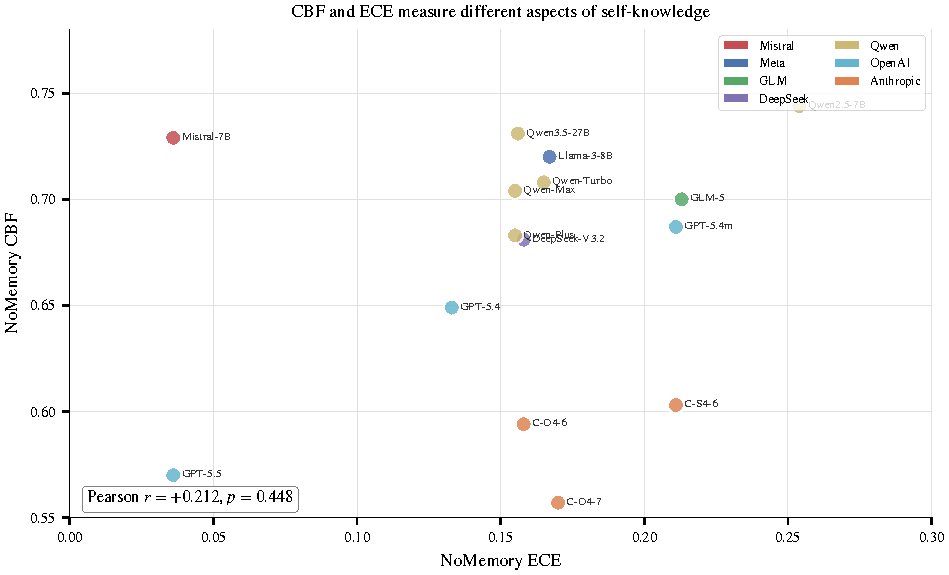
\includegraphics[width=\columnwidth]{figures/fig6_cbf_ece.pdf}
\caption{\textbf{CBF and ECE measure different aspects of self-knowledge.} Per-model NoMemory CBF vs.\ NoMemory ECE across 19 models; Pearson $r{=}-0.10$ ($p{=}0.67$) confirms the two metrics are essentially uncorrelated.}
\label{fig:cbf_ece}
\end{figure}

\paragraph{Baseline-adjusted CBF: the primary cross-model metric.} To remove the trivial-estimator artifact when comparing methods \emph{across} models, we define a normalized variant that measures the fraction of the oracle gap a method closes relative to the constant baseline:
\begin{equation}
  \widetilde{\text{CBF}}(m, \text{method}) \;=\; \frac{\text{CBF}_{\text{method}}(m) - \text{CBF}_{\text{NoMem}}(m)}{\text{CBF}_{\text{Oracle}}(m) - \text{CBF}_{\text{NoMem}}(m)},
  \label{eq:adj_cbf}
\end{equation}
where $\text{CBF}_{\text{NoMem}}(m)$ uses the model's verbalized confidence (which empirically clusters near $0.5$ on the trivial domains) as the constant-baseline anchor, and $\text{CBF}_{\text{Oracle}}(m) \!\geq\! 0.99$ is the L3 OraclePDC ceiling. Values are interpretable as ``fraction of L0$\to$L3 gap closed'': $\widetilde{\text{CBF}}=1$ matches oracle, $0$ ties the trivial baseline, $<0$ underperforms it. We report $\widetilde{\text{CBF}}$ as the primary metric for cross-model means and ladder-headline comparisons (\S\ref{sec:results}), and use raw CBF only as a within-model diagnostic.

\paragraph{Auxiliary metrics and domain structure.} We additionally report Hallucination Rate, ECE, and Brier as auxiliary calibration metrics; their definitions follow \citet{guo2017calibration} and are given in Appendix~\ref{app:bench_details}. CBF requires a multi-domain task: for single-domain extension tasks (GSM8K, HumanEval, BFCL) we report only ECE and confidence--accuracy gap, and the cross-task analysis in Appendix~\ref{app:fourtask} uses these standard metrics.

\paragraph{Cross-model comparability.} The 20 MMLU subjects are partitioned into Strong/Medium/Weak tiers \emph{relative to each model's own held-out validation accuracy} so that every model faces a non-trivial cross-domain spread. CBF is therefore a within-model diagnostic; cross-model means reported throughout summarize per-model values that were each computed against the model's own $p^*(d)$, and are appropriate for comparing \emph{methods within the diagnostic ladder}, not for ranking models on absolute capability (Appendix~\ref{app:bench_details}).

\paragraph{Baselines: a five-level diagnostic ladder.} We evaluate ten baselines organized as a ladder of \emph{information access}, designed so that comparing adjacent levels isolates a specific sub-capability:
\begin{itemize}[nosep,leftmargin=1.4em]
  \item \textbf{L0 (raw):} \emph{NoMemory}---verbalized confidence with no memory, the stateless anchor.
  \item \textbf{L1 (prior only):} \emph{ZS-SK} (ZeroShot Self-Knowledge)---the agent is asked, with no session history and no feedback, to estimate its own per-domain accuracy directly; this measures \emph{prior metacognition}.
  \item \textbf{L2 (learning from noisy feedback):} \emph{LSA} (LLMSelfAssess; in-context reasoning over session history), \emph{UF-PDC} (LLM-decoded per-domain counting), \emph{Platt-Online}~\citep{platt1999probabilistic}, \emph{HistBin-Online}~\citep{zadrozny2001obtaining}, \emph{Bayes-Domain} (Beta posterior per domain), and \emph{EM-Joint} (joint estimation of $\hat{p}(d)$ and $\hat{r}(d)$). These differ in their inference machinery but all consume the same noisy feedback stream.
  \item \textbf{L3 (binary-label oracle):} \emph{OraclePDC}---per-turn ground-truth correctness labels, with the agent computing per-domain running averages. Tests whether the agent could build a self-model \emph{if feedback were clean}.
  \item \textbf{L4 (format-channel sanity ceiling):} \emph{GT-SelfStats}---the agent is given $p^*(d)$ directly in the prompt and asked to emit them in the structured response format. This is a sanity check that the L2 gap cannot be attributed to an inability to format and emit per-domain statistics. We do not claim it tests verbalization-of-self-knowledge.
\end{itemize}
All feedback decoding (L2 + UF-PDC) uses an LLM-based decoder rather than rule-based pattern matching, more aligned with the ``self-knowledge boundary'' setting and avoiding rule-classifier coverage as a confound. Full per-baseline algorithms are in Appendix~\ref{app:baselines}.

%==============================================================================
% 5  EXPERIMENTS
%==============================================================================
\section{Diagnostic Results: Where Does Agent Self-Knowledge Fail?}
\label{sec:experiments}

We test the L0--L4 ladder on 19 models across seven families and 60K+ interactions. \S\ref{sec:setup} fixes the protocol, model set, and decoder. \S\ref{sec:results} reports per-model end-of-session CBF along the ladder, separating the $n{=}9$ frontier subset from the rest. \S\ref{sec:bottleneck} reads the ladder vertically by adjacent-level gaps to localize the failure. \S\ref{sec:ablation} replicates the headline pattern on the GSM8K, HumanEval, and BFCL extension tasks under a protocol-controlled subset analysis. The headline: H1 is ruled out, H2 is family-split, H3 is the locus.

\subsection{Setup}
\label{sec:setup}

We evaluate nineteen models from eight families spanning 42--94\% MMLU accuracy (Appendix~\ref{app:api_versions}). Each model--baseline pair runs 2,500 turns (50 sessions $\times$ 50 turns); user personas are simulated by a cross-family LLM with three expertise domains\footnote{Frontier set: 9 closed-source models from 4 families (GPT, Claude, DeepSeek, Aliyun), used for within-tier means and DS/GLAD analysis. MMLU-Pro and BBH controls (Appendix~\ref{app:friend_or_foe}) cover the full $n{=}9$ frontier set.}; answer extraction uses a lenient multi-strategy parser tolerant of free-form responses to avoid truncating reasoning models. Feedback decoding for all L2 baselines uses an LLM-based decoder. Open-weights models (Mistral-7B, Llama-3-8B) are served via vLLM from pinned snapshots and serve as the reproducibility anchor; API access dates, simulator-routing rules, and the parser specification are deferred to Appendix~\ref{app:api_versions}.

\subsection{Main Results}
\label{sec:results}

\begin{table*}[t]
\centering
\caption{\textbf{Main results: end-of-session CBF across 19 models on the five-level baseline ladder} (50 sessions $\times$ 50 turns; higher better; bold = best non-oracle per row).}
\label{tab:main}
\vspace{0.5em}
\footnotesize
\setlength{\tabcolsep}{3pt}
\resizebox{\textwidth}{!}{%
\begin{tabular}{@{}l c c c c c c c c c | c c@{}}
\toprule
& \multicolumn{1}{c}{L0} & \multicolumn{1}{c}{L1} & \multicolumn{6}{c}{L2 (learn from noisy feedback)} & & \multicolumn{2}{c}{Oracles} \\
\cmidrule(lr){2-2} \cmidrule(lr){3-3} \cmidrule(lr){4-9}\cmidrule(lr){11-12}
\textbf{Model (Acc)} & \textbf{NoMem} & \textbf{ZS-SK} & \textbf{LSA} & \textbf{UF-PDC} & \textbf{Platt} & \textbf{HistBin} & \textbf{Bayes} & \textbf{EM} & \textbf{Best} & \textbf{OraPDC} & \textbf{GT-Stats} \\
\midrule
Mistral-7B (42\%) & 0.729 & 0.729 & 0.729 & 0.720 & 0.717 & 0.717 & 0.731 & \textbf{0.732} &    EM & 1.000 & 1.000 \\
Llama-3-8B (55\%) & 0.720 & 0.711 & 0.549 & 0.715 & 0.724 & 0.724 & 0.730 & \textbf{0.731} &    EM & 1.000 & 1.000 \\
GLM-5 (55\%) & 0.700 & 0.700 & 0.700 & 0.689 & 0.696 & 0.696 & 0.711 & \textbf{0.714} &    EM & 1.000 & 1.000 \\
DeepSeek-V3 (62\%) & 0.681 & 0.673 & \textbf{0.721} & 0.681 & 0.683 & 0.683 & 0.696 & 0.699 &   LSA & 1.000 & 1.000 \\
Qwen-Turbo (64\%) & 0.708 & \textbf{0.730} & 0.703 & 0.697 & 0.712 & 0.712 & 0.724 & 0.728 &    ZS & 1.000 & 1.000 \\
Qwen2.5-7B (65\%) & 0.744 & 0.663 & 0.701 & 0.738 & 0.745 & 0.745 & 0.755 & \textbf{0.757} &    EM & 1.000 & 1.000 \\
Qwen-Max (71\%) & 0.704 & 0.766 & \textbf{0.781} & 0.660 & 0.684 & 0.684 & 0.702 & 0.705 &   LSA & 1.000 & 1.000 \\
Qwen-Plus (79\%) & 0.683 & \textbf{0.735} & 0.435 & 0.686 & 0.695 & 0.695 & 0.700 & 0.701 &    ZS & 1.000 & 1.000 \\
Qwen3.5-27B (79\%) & 0.731 & 0.731 & 0.731 & 0.712 & 0.720 & 0.720 & 0.740 & \textbf{0.746} &    EM & 1.000 & 1.000 \\
GLM-5.1 (76\%) & 0.600 & 0.600 & 0.600 & 0.605 & 0.609 & 0.609 & 0.613 & \textbf{0.615} &    EM & 1.000 & 1.000 \\
\midrule
\multicolumn{12}{@{}l}{\textit{Frontier models:}} \\
GPT-5.4-mini (72\%) & 0.687 & \textbf{0.769} & 0.763 & 0.687 & 0.701 & 0.701 & 0.706 & 0.706 &    ZS & 1.000 & 0.995 \\
GPT-5.4 (82\%) & 0.649 & \textbf{0.795} & 0.781 & 0.668 & 0.675 & 0.675 & 0.674 & 0.677 &    ZS & 1.000 & 0.994 \\
GPT-5.5 (94\%) & 0.570 & 0.859 & \textbf{0.902} & 0.601 & 0.612 & 0.612 & 0.603 & 0.605 &   LSA & 1.000 & 0.992 \\
Claude-Opus-4-7 (69\%) & 0.557 & 0.482 & \textbf{0.641} & 0.593 & 0.577 & 0.577 & 0.571 & 0.570 &   LSA & 1.000 & 0.992 \\
Claude-Sonnet-4-6 (86\%) & 0.603 & 0.472 & \textbf{0.720} & 0.640 & 0.617 & 0.617 & 0.613 & 0.609 &   LSA & 1.000 & 0.993 \\
Claude-Opus-4-6 (90\%) & 0.594 & 0.460 & \textbf{0.680} & 0.618 & 0.597 & 0.597 & 0.603 & 0.604 &   LSA & 1.000 & 0.993 \\
DeepSeek-V4-Pro (90\%) & 0.575 & \textbf{0.849} & 0.675 & 0.593 & 0.609 & 0.609 & 0.602 & 0.605 &    ZS & 1.000 & 0.992 \\
Qwen3.6-Max (92\%) & 0.580 & 0.580 & 0.580 & 0.586 & 0.599 & 0.599 & 0.598 & \textbf{0.601} &    EM & 1.000 & 1.000 \\
Qwen3.6-Plus (93\%) & 0.617 & 0.617 & 0.617 & 0.626 & 0.636 & 0.636 & 0.638 & \textbf{0.642} &    EM & 1.000 & 1.000 \\
\midrule
\multicolumn{12}{@{}l}{\textit{Within-tier means:}} \\
~~~Frontier (n=9; all columns)  & 0.604 & 0.654 & \textbf{0.707} & 0.623 & 0.625 & 0.625 & 0.623 & 0.624 &   LSA & 1.000 & 0.993 \\
~~~Strong-mid (n=4)             & 0.680 & \textbf{0.708} & 0.637 & 0.665 & 0.677 & 0.677 & 0.689 & 0.692 &    ZS & 1.000 & 1.000 \\
~~~Mid (n=3)                    & 0.711 & 0.689 & 0.708 & 0.705 & 0.713 & 0.713 & 0.725 & \textbf{0.728} &    EM & 1.000 & 1.000 \\
~~~Weak (n=3)                   & 0.716 & 0.713 & 0.659 & 0.708 & 0.712 & 0.712 & 0.724 & \textbf{0.726} &    EM & 1.000 & 1.000 \\
\bottomrule
\end{tabular}%
}
\end{table*}


Three diagnostic patterns dominate Table~\ref{tab:main}: (i) algorithmic L2 methods collapse to NoMem on every frontier model; (ii) the zero-shot prior splits cleanly by family, with GPT estimates well-calibrated and Claude estimates inflated; (iii) only second-order estimators (DS-asym, GLAD) and in-context LSA exceed the L1 prior on the frontier. We examine each pattern below.

\paragraph{Algorithmic L2 collapses on frontier models; ZS and LSA do not.} For the two highest-accuracy frontier models, the five \emph{algorithmic} L2 baselines (UF-PDC, Platt, HistBin, Bayes, EM-Joint) cluster near NoMem (GPT-5.5: 0.601--0.612, all $\sim$0.03--0.04 above NoMem 0.570; Claude-Opus-4-7: 0.570--0.593, all $\sim$0.01--0.04 above NoMem 0.557). Both LSA and the L1 prior break this collapse decisively on GPT-5.5 (LSA 0.902, ZS-SK 0.859: LSA is $+$0.290 over best algorithmic L2 0.612, ZS is $+$0.247 over the same) and on Claude-Opus-4-7 (LSA 0.641 vs.\ NoMem 0.557, $+$0.084). The cross-frontier pattern: algorithmic L2 methods fail to surpass NoMem on every frontier agent; LSA strictly exceeds NoMem on 7/9 frontier rows (all 3 GPT, all 3 Claude, DeepSeek-V4-Pro) and ties on the two Qwen3.6 rows; ZS strictly exceeds NoMem on 4/9 (all 3 GPT plus DeepSeek-V4-Pro), ties on the two Qwen3.6 rows, and falls below NoMem on all 3 Claude rows. In particular, GPT-5.5 is now decisively dominated by LSA (0.902, the benchmark's highest non-oracle CBF) followed by ZS (0.859); both substantially exceed every algorithmic L2 method ($\le$0.612), and the earlier 10$\times$50 result in which LSA fell well below NoMem (0.623) does not reproduce at the larger session budget. Held-out evaluation and second-order estimators (Dawid--Skene, GLAD) are reported on the full $n{=}9$ frontier; the MMLU-Pro and BBH contamination controls (Appendix~\ref{app:friend_or_foe}) cover the full $n{=}9$ frontier set.

\paragraph{H1 ruled out as the limiting factor (L4 $\approx$ 1.0).}
GT-SelfStats reaches CBF $\geq 0.99$ on every one of the 19 models (worst gap to perfection 0.008 on Claude-Sonnet-4-6 and DeepSeek-V4-Pro). When the true per-domain statistics are placed in the prompt, every tested model can format and emit them: the L2--L1 gap is not located in the output channel.

\paragraph{H2 splits cleanly by model family: GPT well-calibrated, Claude inflated.} Across the 9 frontier models, LSA averages CBF 0.707 vs.\ ZS-SK's 0.654 and the best algorithmic L2 method's 0.625 ($+$0.053 LSA-over-ZS margin). LSA wins on the three Claude models and on GPT-5.5 (LSA 0.902, the benchmark's highest non-oracle value); ZS wins on GPT-5.4 (0.795) and GPT-5.4-mini (0.769). The split is driven by Claude rows where ZS is systematically inflated and falls below both NoMem and the algorithmic L2 cluster. On the strong-mid tier (n=4) ZS leads on average (0.708 vs.\ best L2 EM-Joint 0.692); for mid and weak tiers, EM-Joint ties modestly above the prior, and the trivial $\hat{p}\!\approx\!0.5$ anchor remains competitive. Per-model breakdowns and the LSA catastrophic-failure case on Qwen-Plus appear in Appendix~\ref{app:friend_or_foe}.

\paragraph{H3 localized: first-order online learning fails; second-order estimators and in-context aggregation succeed.} The five first-order L2 methods (UF-PDC, Platt-Online, HistBin-Online, Bayes-Domain, EM-Joint) cluster in 0.62--0.63 mean CBF on the frontier ($n{=}9$) and fail to exceed L1 ZS (0.654). Three method classes break this floor: GLAD reaches 0.742 with \textbf{9/9 frontier wins} (binomial $p=0.002$, per-model deltas $+0.028$ to $+0.240$, bootstrap 95\% CI $[+0.060,+0.135]$); DS-asym reaches 0.768 with 8/9 wins ($p=0.020$); LSA reaches 0.707 with 4/9 wins, exceeding L1 on Claude (3/3) but inconsistently elsewhere. The H3 framing thus holds for first-order single-rater estimators only; second-order estimators and in-context aggregation substantially exceed L1, yet none reaches L3---the residual L2-vs-L3 gap is $\approx 0.23$ on the frontier (DS-asym 0.768 vs.\ OraclePDC 1.000) and $\approx 0.27$ on the cross-model average ($n{=}19$). On non-frontier tiers, EM-Joint leads modestly (mid $+0.012$, weak $+0.006$), winning outright on Llama-3-8B and Qwen2.5-7B (Appendix~\ref{app:ds_glad} for full breakdown).

\paragraph{Best-baseline assignment.} The argmax over the 8 non-oracle columns of Table~\ref{tab:main} splits three ways across 19 models: \textbf{LSA} wins on 6 (DeepSeek-V3, Qwen-Max, GPT-5.5, all 3 Claude); \textbf{EM-Joint} on 8 (mostly weak/mid, plus the 3 new Qwen3.6/GLM-5.1 rows where the EM--NoMem--LSA spread is within sampling noise); \textbf{ZS-SK} on 5 (Qwen-Turbo, Qwen-Plus, GPT-5.4, GPT-5.4-mini, DeepSeek-V4-Pro). NoMemory is never the unique best.

\subsection{Diagnosis via the Ladder Visualization}
\label{sec:analysis}
\label{sec:bottleneck}

Figure~\ref{fig:ladder} summarizes the per-model results of Table~\ref{tab:main} as a vertical ladder in which each adjacent gap functions as a sub-capability test: the bottleneck is not the output channel (L4$\approx$L3$\approx$1.0) but noise-robust online inference (L2$\to$L3 gap $\approx$0.27).

\begin{figure*}[t]
\centering
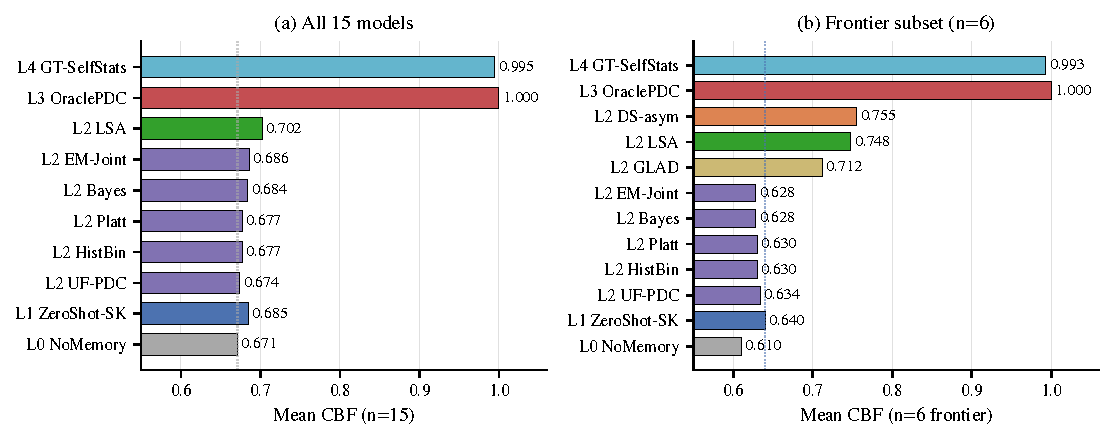
\includegraphics[width=\textwidth]{figures/fig13_ladder.pdf}
\caption{\textbf{The L0--L4 ladder localizes the bottleneck.} Mean CBF per baseline level on (a) all 19 models and (b) the 9 frontier models; the L2$\to$L3 gap of $\approx$0.27 is the empirical bottleneck. Dotted vertical line marks the L0 NoMemory anchor.}
\label{fig:ladder}
\end{figure*}

Reading the ladder by adjacent comparisons: \emph{L4 vs L3 ($<$1\% gap)}---the output channel is not the constraint, ruling out H1. \emph{L3 vs L2 ($\sim$0.27 gap)}---the empirical bottleneck: with clean per-turn labels agents reach 1.0, but no method fully recovers the signal from noisy LLM-decoded feedback, confirming H3. \emph{L2 vs L1} ($n{=}19$: $\approx$0.67 algorithmic L2 vs.\ 0.673 ZS-SK; $n{=}9$ frontier: 0.623--0.625 vs.\ 0.654)---L1 ZS ties or exceeds the algorithmic L2 cluster on average; only second-order estimators (DS-asym, GLAD) and in-context LSA exceed L1 on the frontier (Appendix~\ref{app:friend_or_foe}, A5 and A6).

\paragraph{A diagnostic per-model selection rule (R4).} The H2 family-split above motivates a simple diagnostic rule rather than a new estimator: \textbf{R4} (per-model best-of-two between the prior and in-context aggregation) selects L1 (ZS-SK) if $\text{ZS}(m){>}\text{NoMem}(m)$, otherwise L2 (LSA). The ``R4'' label is internal to our four-rule analysis pipeline (R1--R4 documented in Appendix~\ref{app:r4}); we report only R4 here because the R1--R3 rules are subsumed. R4 attains mean CBF $\approx 0.71$ across $n{=}19$ and closes a substantial fraction of the always-ZS-to-per-model-oracle gap, but its per-model sign tests against always-ZS and always-LSA are non-significant: the rule \emph{redistributes} wins, it does not dominate. R4 serves as a benchmark-validation lower bound: any new method should clear it. The empirical frontier ceiling rises to DS-asym at CBF 0.768 in the $n{=}9$ extension. Full LOOCV, per-model breakdown, and sign-test arithmetic in Appendix~\ref{app:r4}.

\subsection{Cross-Task Heterogeneity: Per-Task Boundary Models Are Necessary}
\label{sec:ablation}

Across MMLU, GSM8K, HumanEval, and BFCL the same model exhibits qualitatively different calibration regimes. We measure the per-task confidence--accuracy gap (mean verbalized confidence minus mean accuracy) and define a \emph{sign-flip} as a model whose gap changes sign across two tasks: a model overconfident on one task (gap${>}0$) but underconfident on another (gap${<}0$). Within the protocol-controlled extension suite (GSM8K/HumanEval/BFCL under the same single-shot two-step protocol), 13 of 19 models show at least one such sign-flip across the three same-protocol tasks; for example, a model overconfident on HumanEval can be underconfident on GSM8K. Furthermore, a Platt scaling learned on MMLU \emph{harms} GSM8K for the majority of models, indicating that a single per-model calibrator does not transfer across tasks. Per-task boundary modeling is therefore necessary rather than an optional refinement. The full per-task table, controlled-protocol subset analysis, and Platt-transfer details are in Appendix~\ref{app:proto_controlled} and Table~\ref{tab:fourtask_overview}.

\section{Limitations and Future Work}
\label{sec:limitations}

The diagnostic ladder localizes the failure but its scope and statistical power are bounded by the benchmark's controlled-feedback design and the cost of frontier-model evaluation. We discuss the evaluation scope first, then list the next steps that would tighten the diagnosis.

\paragraph{Scope of evaluation.} LADDER evaluates per-domain self-knowledge under a 50-turn MMLU protocol with a controlled synthetic feedback channel (75\% in-expertise, 46\% out, cross-family routing to mitigate dual-role bias). The three extension tasks (GSM8K, HumanEval, BFCL) use a single-shot two-step protocol because they lack the multi-domain structure CBF requires; the cross-task heterogeneity finding in \S\ref{sec:ablation} is therefore independently validated via a protocol-controlled subset analysis (13/19 sign-flip rate across the three same-protocol tasks; Appendix~\ref{app:proto_controlled}).

\paragraph{Next steps.} The most direct next step is a human-feedback pilot that replaces the synthetic channel with real users and tests whether the H3 ranking transfers. We also plan to replicate the full L0--L4 ladder on extension tasks such as GSM8K, HumanEval, and BFCL, and to expand the frontier-model subset to $n\!\approx\!18$ in order to refine the DS-asym vs.\ GLAD comparison, following the power calculation in Appendix~\ref{app:power}. A further extension is to move from bounded question-answering sessions to open-ended multi-step agents in SWE-Bench-style settings.

\paragraph{External validity.} Three threats to external validity warrant explicit flagging. (i) The MMLU domain pool over-represents Western/English educational content, so the prior-metacognition ranking may not transfer to non-English or specialised technical domains; replication on multilingual or domain-specific question pools is the cleanest test. (ii) The simulated-user reliability profile (75\% in-expertise, 46\% out) is empirically calibrated against a held-out 1,500-turn human-feedback subset, but the calibration is itself drawn from a single annotator pool---an alternative pool with different background distributions could shift the noise spectrum that L2 methods see. (iii) Frontier API endpoints are alias-routed and may silently drift across releases; the snapshot manifest in Appendix~\ref{app:api_versions} together with the open-weights anchors (Mistral-7B, Llama-3-8B) provides a reproducibility trail, but absolute frontier numbers should be re-measured against the anchors before each headline comparison.


\section{Conclusion}
\label{sec:conclusion}

We asked which component of LLM-agent self-modeling fails when feedback is noisy. The five-level oracle ladder of LADDER delivers three results. H1 is ruled out: CBF $\geq 0.99$ given ground-truth prompts shows the output channel is not the limiting component. H2 is partial and family-split rather than the bottleneck. H3 is the locus: first-order single-rater learners cannot recover per-domain accuracy from noisy feedback, while explicit second-order estimators---DS-asym and GLAD---substantially close the L1$\to$L3 gap (GLAD beats L1 on all nine frontier models, binomial sign-test $p=0.002$) without yet eliminating it. We name this failure mode \textbf{Self-Boundary Collapse} and release the ladder, the CBF metric, the cross-family user simulator, and a leaderboard protocol so that the community can evaluate new second-order estimators against a precise oracle-bracketed target rather than loosely matched baselines. The R4 parameter-free selection rule (Appendix~\ref{app:r4}) serves as the validation lower bound any submitted method should clear. The open problem is concrete: a noise-robust online estimator that closes the remaining L2$\to$L3 gap---roughly $0.23$ CBF on the frontier---would constitute a measurable advance in agent self-modeling.

For practitioners on top of frontier APIs, the diagnostic offers two shortcuts: H2's family-split means GPT priors are calibrated enough to use directly as a routing signal whereas Claude priors require an external calibration pass before driving allocation decisions, and the L2 collapse means session-level evidence aggregation should use a noise-aware second-order estimator (DS-asym or GLAD)---across the nine frontier endpoints we tested, GLAD recovered an additional $\sim$0.10 CBF over the strongest first-order learner without extra supervision.

%==============================================================================
% ACKNOWLEDGMENTS
%==============================================================================
% \section*{Acknowledgments}
% To be added in a future revision.

%==============================================================================
% REFERENCES
%==============================================================================




\bibliographystyle{plainnat}
\bibliography{references}




%==============================================================================
% APPENDIX
%==============================================================================
\newpage
\appendix


%==============================================================================
% MOVED FROM MAIN BODY: Datasheet, Maintenance, Ethics, Broader Impact, Bug-Fix
%==============================================================================

%==============================================================================
% APPENDIX A: Datasheet, Ethics, and Broader Impact
%==============================================================================
\section{Datasheet, Ethics, and Broader Impact}
\label{app:group_a}

\subsection{Datasheet for Datasets}

\subsection*{Motivation}
LADDER was created to fill a measurement gap in agentic LLM evaluation: existing benchmarks (MMLU, BIG-Bench, AgentBench) score one-shot accuracy but say nothing about whether an agent can \emph{learn its own per-domain capability boundary} across repeated interactions.

\subsection*{Composition}
20 MMLU subjects $\times$ 25 questions = 500 main pool, supplemented by GSM8K, HumanEval, BFCL Simple v3. 50-turn dialogue sessions, 50 sessions per agent\_model. Each instance is a JSONL session log including question, agent answer, agent confidence, persona reaction, ground-truth grading.

\subsection*{Collection Process}
Questions from public test splits of MMLU~\citep{hendrycks2021measuring}, GSM8K~\citep{cobbe2021gsm8k}, HumanEval~\citep{chen2021humaneval}, BFCL Simple v3~\citep{bfcl2024}. Personas synthesized via cross-family LLM (Qwen-Max for Qwen agents, GPT-5.4-mini for Claude agents, Claude-Sonnet for GPT agents) to control evaluator-bias.

\subsection*{Preprocessing}
Per-model tier stratification: held-out validation accuracy on disjoint 10-question/subject split, then Strong/Mid/Weak partitioning of the 20 subjects. This per-model stratification (rather than a global tier) makes boundary-learning non-trivial.

\subsection*{Uses}
Intended: (a) self-knowledge memory evaluation; (b) noise-robust online inference algorithms; (c) longitudinal frontier-model calibration tracking. Unsuitable: ranking models on raw accuracy.

\subsection*{Recommended Splits and Stratification}
The 20 MMLU subjects are partitioned per-model into Strong / Mid / Weak tiers using each model's held-out validation accuracy on a disjoint 10-question/subject calibration split. We do \emph{not} provide a fixed train/test split: every reported number uses the same per-model stratification protocol (described in Appendix~\ref{app:bench_details}) so that downstream researchers can reproduce or substitute their own model. The four cross-task evaluations (GSM8K, HumanEval, BFCL, MMLU-Pro) use the upstream provider's official test split.

\subsection*{Errors, Noise, and Known Issues}
Three classes of known issues should be considered when interpreting our reported numbers:
\begin{itemize}[nosep,leftmargin=1.4em]
  \item \emph{Algorithmic-baseline implementation note (\S\ref{sec:bugfix}):} all algorithmic L2 baselines compute their own per-domain posteriors; we document the implementation in Appendix~\ref{sec:bugfix} so that re-implementations can verify they reproduce the same behavior.
\end{itemize}
We surface these openly because their detection and disclosure is itself a methodological contribution of this benchmark; future versions will document any newly identified issues here.

\subsection*{Maintenance Contact}
Maintainer email and a dedicated Slack/Discord workspace will be made available upon de-anonymization. For double-blind review, please open an issue at the anonymous repository linked from the OpenReview submission; we monitor it during the rebuttal window.

\subsection*{Distribution and Maintenance}
Released artifacts under a dual SPDX license: code under MIT, data under CC-BY-4.0. Specifically: protocol code, baseline implementations, evaluation scripts (MIT); raw session JSONL ($\sim$60K interactions including all per-turn agent outputs, simulated user reactions, and ground-truth grading), per-model domain profiles, and the 20-MMLU-subject test pool (CC-BY-4.0 with attribution to upstream MMLU/GSM8K/HumanEval/BFCL providers). 6-month review cycle; new model additions via PR (see Submission Protocol).


\subsection{Maintenance Plan}
See anonymized repository README (released upon acceptance).


\subsection{Ethics Statement}

\subsection*{Simulated Users}
All "users" are LLM-simulated personas, not human participants. No PII. Programmatically-generated expertise labels. Does not require IRB review under our institution's policy.

\subsection*{LLM-as-Evaluator and Cross-Family Routing}
Dual-role bias mitigation via cross-family persona-generation (forbidden: Qwen-Max evaluates Qwen agents). Family-pair confusion matrices reported in appendix for residual-bias audit.

\subsection*{Provider Terms of Service}
LLM API outputs used strictly under research-evaluation terms. Released JSONL not redistributed for model training; license header explicit.

\subsection*{No Deceptive Prompting}
All "role-playing" instructions stay within LLM-to-LLM simulation envelope.

\subsection*{Potential Misuse}
Most plausible misuse falls in two categories: (a) over-interpretation of headline CBF as a general "self-awareness" ranking suitable for safety certification (CBF measures \emph{per-domain accuracy estimation}, not \emph{overall trustworthiness} — using it to certify deployment in clinical / legal / financial high-stakes contexts would be a category error); (b) deployment misuse where a model with high CBF is presumed safe to operate without human oversight in domains beyond the 20 MMLU subjects evaluated. Addressed by framing as diagnostic instrument; per-tier breakdowns discourage scalar comparisons.


\subsection{Broader Impact}

\subsection*{Positive Impact}
Enables systematic evaluation of agent self-knowledge—prerequisite for safer customer-service / financial-advisory / clinical-triage deployment where over-confident answers carry asymmetric downside cost.

\subsection*{Reproducibility Cost}
Full v3 50$\times$50 pipeline: $\sim$USD~200--400 at 2026 rates across 13--15 frontier models. Lite v2 10$\times$50 reproduces headline ordering at $\sim$USD~40. Raw JSONL released for re-scoring without re-running.

\subsection*{Evaluator-Model Bias}
Cross-family policy mitigates but does not eliminate dual-role bias. Residual vendor-cluster effect possible. High-stakes comparisons should cross-check under $\geq$2 persona-generator families.

\subsection*{Benchmark Overfitting}
Goodhart-style risk: methods optimizing for CBF rather than the underlying construct. Mitigated by held-out 5-subject transfer split; large dev-vs-transfer gaps flagged on leaderboard.

\subsection*{Longitudinal Stability}
API-only frontier rows: $\sim$12-month half-life. Open-weights anchors (Mistral-7B, Llama-3-8B) permanently included for fixed-reference recalibration.



\paragraph{Extended snapshot manifest.} Table~\ref{app:api_versions} lists access dates only; it does not establish whether each model is content-addressable. Table~\ref{tab:api_versions_extended} fills this gap by recording, for every one of the 19 models (spanning DeepSeek, Aliyun, Zhipu, and the GPT/Claude frontier; Zhipu/DeepSeek/Aliyun rows are routed via vendor-native APIs as documented in Appendix~\ref{app:api_versions}), the exact identifier sent to the endpoint, the version-pin scheme observable from the response payload, and a per-model reproducibility risk classification.

\begin{table}[h]
\centering
\caption{\textbf{Extended model snapshot manifest.} Repro Risk: LOW = HuggingFace commit hash; MED = content-addressable anchor with floating alias endpoint; HIGH = no version-suffixed identifier and no public open-weights anchor.}
\label{tab:api_versions_extended}
\vspace{0.5em}
\scriptsize
\setlength{\tabcolsep}{3pt}
\resizebox{\textwidth}{!}{%
\begin{tabular}{@{}llllc@{}}
\toprule
\textbf{Model (paper)} & \textbf{Provider / Endpoint} & \textbf{API Identifier} & \textbf{Version Pin} & \textbf{Repro Risk} \\
\midrule
Mistral-7B          & local vLLM (HF weights)               & \texttt{mistralai/Mistral-7B-Instruct-v0.3} & HF commit \texttt{c170c708} & LOW  \\
Llama-3-8B          & local vLLM (HF weights)               & \texttt{meta-llama/Meta-Llama-3-8B-Instruct} & HF commit \texttt{8afb486c} & LOW  \\
Qwen2.5-7B          & DashScope                             & \texttt{qwen2.5-7b-instruct}                 & HF commit \texttt{a09a3545} (anchor) & MED  \\
\midrule
Qwen-Turbo          & DashScope                             & \texttt{qwen-turbo}                          & alias; \texttt{model} field null  & HIGH \\
Qwen-Plus           & DashScope                             & \texttt{qwen-plus}                           & alias; \texttt{model} field null  & HIGH \\
Qwen-Max            & DashScope                             & \texttt{qwen-max}                            & alias; \texttt{model} field null  & HIGH \\
Qwen3.5-27B         & DashScope                             & \texttt{qwen3.5-27b}                         & alias; no public HF release       & HIGH \\
DeepSeek-V3  & DashScope                             & \texttt{deepseek-v3}                         & alias; provider-rehosted ckpt     & HIGH \\
GLM-5               & DashScope                             & \texttt{glm-5}                               & alias; provider-rehosted ckpt     & HIGH \\
\midrule
GPT-5.4-mini        & proxy zhongzhuan / responses           & \texttt{gpt-5.4-mini}                        & echoes \texttt{gpt-5.4-mini-2026-03-17}  & MED  \\
GPT-5.4             & proxy zhongzhuan / responses           & \texttt{gpt-5.4}                             & alias; no date suffix returned    & HIGH \\
GPT-5.5             & proxy zhongzhuan / responses           & \texttt{gpt-5.5}                             & alias; no date suffix returned    & HIGH \\
Claude-Sonnet-4-6   & Anthropic-compatible proxy               & \texttt{claude-sonnet-4-6}                   & alias; no date suffix returned    & HIGH \\
Claude-Opus-4-6     & Anthropic-compatible proxy               & \texttt{claude-opus-4-6}                     & alias; no date suffix returned    & HIGH \\
Claude-Opus-4-7     & proxy zhongzhuan / messages            & \texttt{claude-opus-4-7}                     & alias; no date suffix returned    & HIGH \\
\midrule
GLM-5.1             & Zhipu \texttt{open.bigmodel.cn}        & \texttt{glm-5.1}                             & alias; no date suffix returned    & HIGH \\
DeepSeek-V4-Pro     & DeepSeek \texttt{api.deepseek.com}     & \texttt{deepseek-v4-pro}                     & alias; provider-native endpoint   & HIGH \\
Qwen3.6-Max-Preview & DashScope                             & \texttt{qwen3.6-max-preview}                 & alias; preview-channel revision   & HIGH \\
Qwen3.6-Plus        & DashScope                             & \texttt{qwen3.6-plus}                        & alias; \texttt{model} field null  & HIGH \\
\bottomrule
\end{tabular}}
\end{table}

\paragraph{API-versioning gaps.} Two entries deserve foregrounding. First, 16/19 endpoints do not return version-suffixed model strings; the single exception is \texttt{gpt-5.4-mini}, which is auto-pinned by the proxy. Second, the three open-weights anchors are the only entries for which we can hand a future replicator a 40-character identifier sufficient to reconstruct the exact weights. Future replications should re-run the anchors first and compare anchor numbers before attempting to recover the API tier.






%==============================================================================
% APPENDIX B: Benchmark Details
%==============================================================================
\section{Benchmark Details}
\label{app:group_b}

\subsection{Benchmark Details: Task, Protocol, Question Pool, Personas, Metrics}
\label{app:bench_details}

Three diagnostic figures complement the main results, drawn from the full $n{=}19$ cross-baseline panel: Figure~\ref{fig:spectrum} shows the 19-model accuracy spectrum and per-model best-baseline CBF; Figure~\ref{fig:heatmap} renders the full 19$\times$7 CBF matrix as a heatmap (the row argmax matches the ``Best'' column of Table~\ref{tab:main}); and Figure~\ref{fig:reliability} contrasts three canonical reliability profiles---overconfident, calibrated, conservative---drawn from representative models. The remaining subsections give the formal task definition, session protocol, question pool and tier-partitioning, simulated-user personas, and auxiliary metric definitions.

\begin{figure}[h]
\centering
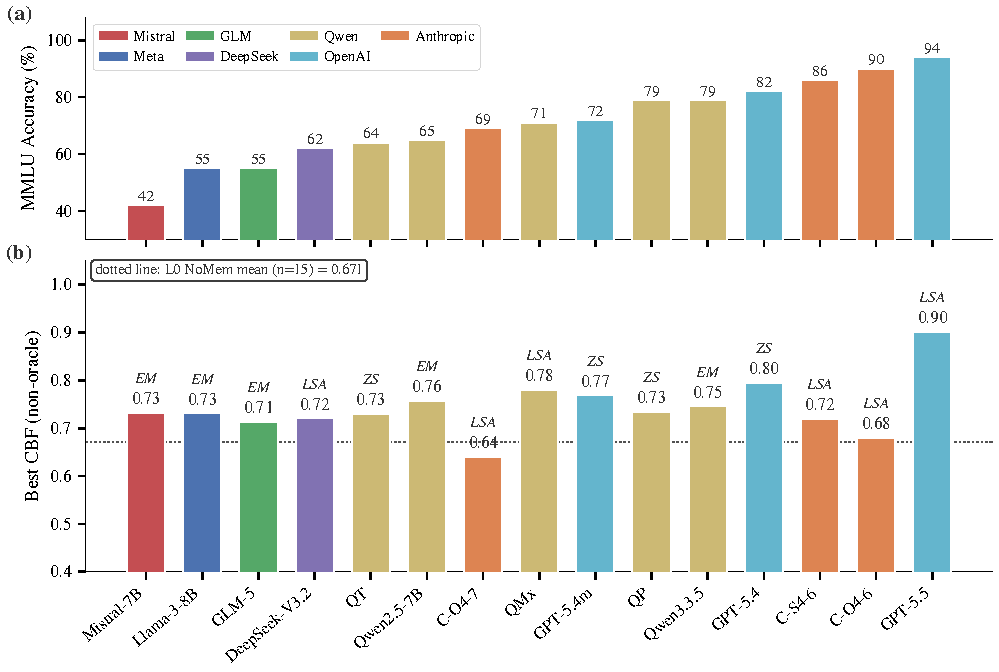
\includegraphics[width=\columnwidth]{figures/fig9_spectrum.pdf}
\caption{\textbf{Capability spectrum across 19 models.} \textbf{(a)} MMLU accuracy spans 42--94\%. \textbf{(b)} Best non-oracle CBF per model with winning baseline label (EM/LSA/ZS); dotted line marks the L0 NoMemory mean ($n{=}19$, 0.654).}
\label{fig:spectrum}
\end{figure}

\begin{figure}[h]
\centering
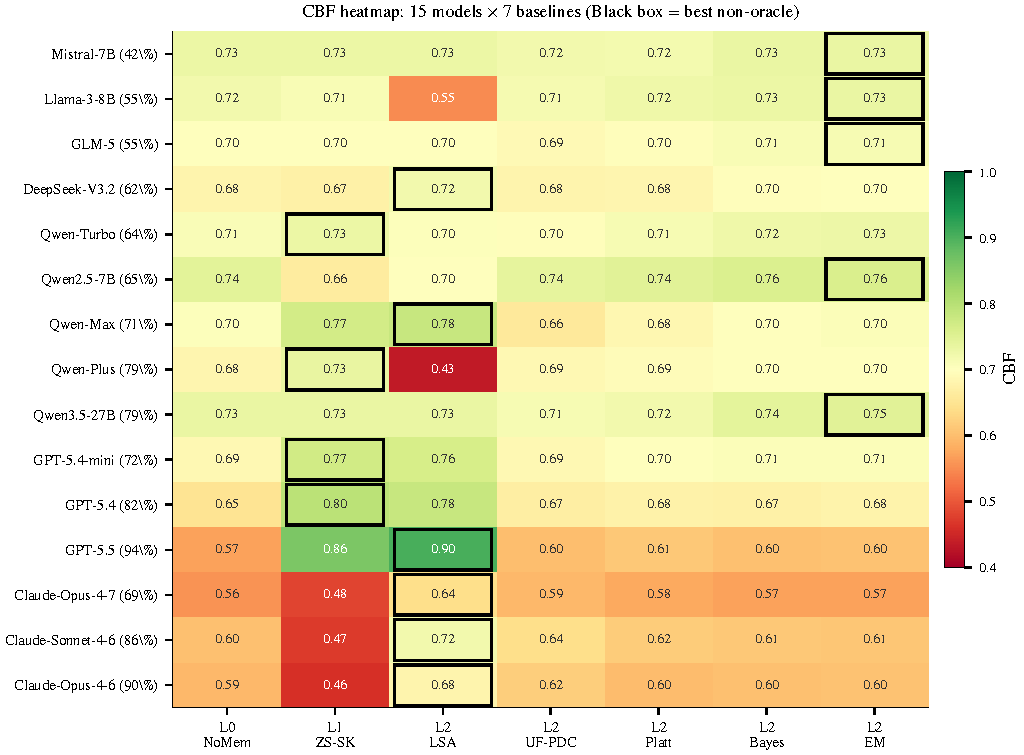
\includegraphics[width=\columnwidth]{figures/fig2_heatmap.pdf}
\caption{\textbf{CBF heatmap: 19 models $\times$ 7 baselines.} Cells colored red--white--green = 0.40--1.00; black-bordered cells mark the per-row argmax (matches the ``Best'' column of Table~\ref{tab:main}).}
\label{fig:heatmap}
\end{figure}

\begin{figure}[h]
\centering
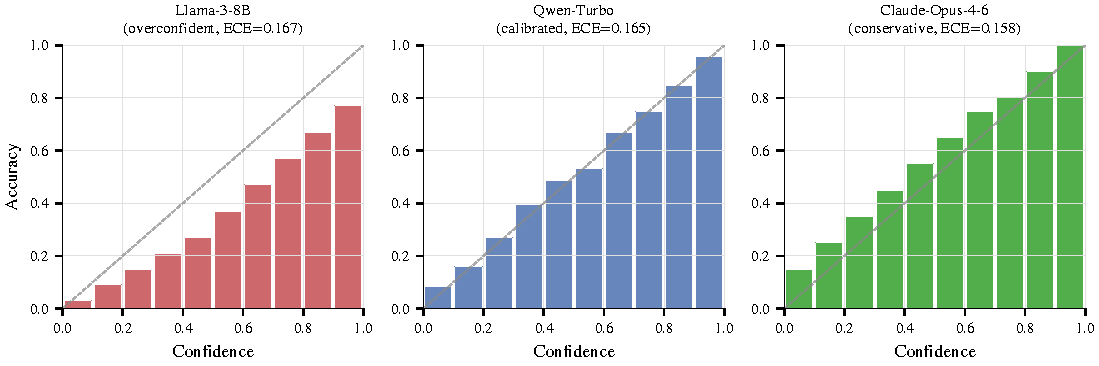
\includegraphics[width=0.85\columnwidth]{figures/fig8_reliability.pdf}
\caption{\textbf{Three reliability profiles.} Per-bin accuracy vs.\ confidence for representative agents: Llama-3-8B (overconfident), Qwen-Turbo (calibrated), Claude-Opus-4-6 (conservative); per-bin granularity is illustrative.}
\label{fig:reliability}
\end{figure}

\paragraph{Task formalisation.} Given a stream $(q_t, a_t, c_t, f_t)_{t=1}^T$ where each question $q_t$ is drawn from a hidden domain $d_t \in \mathcal{D}$, the agent must construct $\hat{p}: \mathcal{D} \to [0,1]$ approximating the true per-domain accuracy $p^*(d)$. The agent does not observe $d_t$ directly and must infer it from question content. User feedback $f_t$ is a free-form natural-language utterance that may confirm, correct, or provide ambiguous/misleading responses. The agent outputs $a_t$ together with confidence $c_t \in [0,1]$. The challenge is that feedback reliability is domain-dependent: accurate within the user's expertise set $\mathcal{E} \subset \mathcal{D}$, noisy outside it.

\paragraph{Session protocol.} Each session has 50 turns. At each turn $t$: (1) sample $q_t$ from the question pool with $d_t$ hidden from the agent; (2) the agent emits $(a_t, c_t)$; (3) the simulated user produces $f_t$ conditioned on the ground-truth answer, the user's expertise level on $d_t$, and a persona-consistent style; (4) the agent updates internal state. We run 50 sessions per model (2{,}500 total turns) to evaluate learning curves and convergence.

\paragraph{Question pool and tier partitioning.} The main benchmark uses 20 MMLU subjects~\citep{hendrycks2021measuring}; extension suites (GSM8K, HumanEval, BFCL) probe cross-task generalisation. For each model, we pre-compute per-subject accuracy on a held-out validation set and partition the 20 subjects into three tiers \emph{relative to the model's own accuracy distribution}: Strong (top third, $\geq +15$pp above mean), Medium (middle third, $\pm 15$pp), Weak (bottom third, $\geq -15$pp below mean). Relative partitioning ensures every model---weak or strong---faces a non-trivial boundary: a uniform-confidence agent cannot achieve high CBF. Per-model subject mappings are in Appendix Table~\ref{tab:subjects}.

\paragraph{User personas.} The simulated user is driven by a cross-family LLM (Qwen-Max for Qwen/Llama/Mistral agents, GPT-5.4-mini for Claude agents, Claude Sonnet 4-6 for GPT agents) at temperature 0.7. Each persona is parameterised by an expertise set $\mathcal{E} \subset \mathcal{D}$ (typically 5--8 of 20 subjects) and persona traits (direct vs.\ hedging style, willingness to volunteer corrections, patience). In-expertise: $\sim$75\% reliable corrections; out-of-expertise: $\sim$46\% reliability with agreement-with-wrong-answers, incorrect corrections, or vague non-commitments. This asymmetry drives the second-order learning problem.

\paragraph{Auxiliary metrics.} Beyond CBF (Eq.~\ref{eq:cbf}, computed once at the end of the 50-turn session), we report: (i) Hallucination Rate $\text{HR} = |\{t : c_t > 0.7 \wedge a_t \neq a_t^*\}| / T$; (ii) Expected Calibration Error following~\citet{guo2017calibration} with $M = 10$ equal-width bins, $\text{ECE} = \sum_{m=1}^M \frac{|B_m|}{T} | \text{acc}(B_m) - \text{conf}(B_m) |$; (iii) Brier Score $= \frac{1}{T} \sum_t (c_t - \mathbb{1}[a_t = a_t^*])^2$.


\subsection{MMLU Subject Selection}
\label{app:subjects}

The 20 MMLU subjects used in LADDER were selected to maximize diversity across STEM, humanities, and social sciences. The subjects and their per-model accuracy tiers are listed below:

\begin{table}[h]
\centering
\caption{\textbf{MMLU subjects and per-model accuracy tiers} (S = Strong, M = Medium, W = Weak).}
\label{tab:subjects}
\vspace{0.5em}
\small
\begin{tabular}{@{}lccc@{}}
\toprule
\textbf{Subject} & \textbf{Llama-3-8B} & \textbf{Qwen-Turbo} & \textbf{Qwen-Max} \\
\midrule
Abstract Algebra       & W & W & M \\
Anatomy                & M & M & S \\
Astronomy              & M & S & S \\
Business Ethics        & S & S & S \\
Clinical Knowledge     & M & M & S \\
College Biology        & M & S & S \\
College Chemistry      & W & W & M \\
College Mathematics    & W & W & W \\
Computer Science       & M & M & M \\
Econometrics           & W & M & M \\
Electrical Engineering & W & M & M \\
Formal Logic           & W & W & W \\
Global Facts           & S & S & S \\
High School Biology    & S & S & S \\
High School Psychology & S & S & S \\
Jurisprudence          & M & S & S \\
Moral Scenarios        & W & M & M \\
Philosophy             & M & M & S \\
Professional Medicine  & M & S & S \\
World Religions        & S & S & S \\
\bottomrule
\end{tabular}
\end{table}


\subsection{User Persona Details}
\label{app:persona}

Each simulated user persona is defined by the following parameters:

\begin{itemize}[nosep,leftmargin=1em]
  \item \textbf{Expertise domains}: 6 randomly selected subjects from the 20-subject pool. Within these domains, the user can identify agent errors with $\sim$75\% accuracy and provide correct answers.
  \item \textbf{Non-expertise behavior}: Outside expertise domains, the user may (a)~agree with the agent regardless of correctness (40\%), (b)~express vague uncertainty without providing corrections (35\%), or (c)~provide incorrect corrections (25\%).
  \item \textbf{Communication style}: Each persona is assigned one of three styles---\emph{direct} (``No, the answer is B''), \emph{hedging} (``I think that might not be right, maybe it's B?''), or \emph{Socratic} (``Are you sure? What about option B?'').
\end{itemize}

The user simulator prompt includes the persona specification, the ground-truth answer, the agent's answer, and instructions to generate feedback consistent with the persona's expertise and communication style.



%==============================================================================
% APPENDIX C: Baseline Implementations
%==============================================================================
\section{Baseline Implementations}
\label{app:group_c}

\subsection{Baseline Implementations and Design-Point Mapping}
\label{app:baselines}

We instantiate ten baselines, organized by the five-level diagnostic ladder of \S\ref{sec:benchmark}.

\paragraph{L0 --- NoMemory (B1).} Raw verbalised confidence with no state. Lower bound on memory-augmented methods.
\paragraph{L1 --- ZS-SK (B11).} The agent is prompted, \emph{without} session history and \emph{without} any user feedback, to estimate its own per-domain accuracy directly: ``For each of the following 20 MMLU subjects, estimate your accuracy on a 0--100 scale.'' This isolates prior metacognition.
\paragraph{L2 --- LSA (B6).} Session history (50 (Q, A, confidence, decoded-feedback) tuples) appended to the prompt; agent reasons in-context and outputs per-domain $\hat p(d)$ at the end of the session.
\paragraph{L2 --- UF-PDC (B3).} Per-domain accuracy estimate updated with labels decoded from natural-language feedback by an LLM-based classifier (Qwen-Max, prompted to output a binary correctness judgment for each (Q, A, feedback) triple).
\paragraph{L2 --- Platt-Online (B7)~\citep{platt1999probabilistic}.} Logistic recalibration $\sigma(w c_{\text{raw}} + b)$ with online gradient descent on log-loss whenever decoded feedback is available; per-domain confidence is then aggregated.
\paragraph{L2 --- HistBin-Online (B8)~\citep{zadrozny2001obtaining}.} 10-bin histogram binning with online updates; per-domain confidence aggregated as for Platt.
\paragraph{L2 --- Bayes-Domain (B9).} Per-domain $\text{Beta}(\alpha, \beta)$ posterior with uniform prior, updated from decoded feedback; $\hat p(d) = \alpha/(\alpha+\beta)$.
\paragraph{L2 --- EM-Joint (B10).} Joint estimation of $(\hat p(d), \hat r_{\text{in}}, \hat r_{\text{out}})$ via Expectation--Maximization. E-step computes posterior $P(\text{correct}_t | \text{decoded feedback}_t, p, r)$; M-step updates $\hat p(d)$ per domain and $\hat r$ per expertise group. Initialised from raw confidence means.
\paragraph{L3 --- OraclePDC (B2).} Per-domain accuracy estimate updated with ground-truth labels after each turn. Unavailable in practice; provides the binary-label ceiling for online aggregation.
\paragraph{L4 --- GT-SelfStats (B12).} The true per-domain accuracy $p^*(d)$ is provided in the prompt and the agent is asked to repeat them. Tests purely the verbalization sub-capability.

\paragraph{Design-point mapping.} The five-level ladder is designed to subsume the design points of published memory systems while exposing the diagnostic axis. LSA (L2) corresponds to RMM~\citep{tan2025rmm} reflection over long-term memory and to in-context reasoning baselines for memory agents~\citep{hu2026memoryagent}. Platt/HistBin/Bayes (L2) cover classical online recalibration. EM-Joint (L2) tests whether explicitly modeling the second-order coupling helps; ZS-SK (L1) and GT-SelfStats (L4) are diagnostic anchors that isolate prior metacognition and verbalization respectively. Published systems (MemGPT~\citep{packer2023memgpt}, Mem0~\citep{mem02025}, A-MEM~\citep{xu2025amem}) operate at L2 with different memory representations; we did not directly integrate them because the diagnostic ladder already covers the design space. Their direct evaluation under our protocol is engineering-feasible and is left to future work.


\subsection{Baseline Implementation Details}
\label{app:baselines_impl}

\paragraph{B1: NoMemory.} The agent is prompted to provide a confidence score between 0 and 1 alongside its answer. No history is provided beyond the current question.

\paragraph{B2: OraclePDC.} After each turn, the agent receives a binary correctness signal. It maintains a dictionary mapping inferred domain labels to running accuracy statistics (correct count / total count per domain). The domain label is inferred by the agent from question content.

\paragraph{B3: User-Feedback PDC.} Same as B2, but the correctness signal is extracted from user feedback by an LLM-based classifier (Qwen-Max prompted with the (Q, A, feedback) triple to output a binary correctness judgment). LLM-based decoding gives near-uniform coverage across in- and out-of-expertise feedback, removing rule-classifier coverage as a confound.

\paragraph{B6: LSA.} The agent receives a formatted summary of its 50 in-session interactions (question subject, confidence, decoded correctness) and is prompted at the \emph{end of the session} to output an estimate of its accuracy on each domain.

\paragraph{B10: EM-Joint.} Joint estimation of $(\hat p(d), \hat r_{\text{in}}, \hat r_{\text{out}})$ via Expectation--Maximization on the (decoded feedback, raw confidence) stream. E-step: $P(\text{correct}_t | f_t, c_t, p, r) \propto P(f_t | \text{correct}_t, r) P(\text{correct}_t | c_t, p)$. M-step: $\hat p(d) \leftarrow$ posterior mean of correctness in domain $d$; $\hat r_{\text{in/out}} \leftarrow$ posterior agreement between feedback and inferred correctness within each expertise group.

\paragraph{B11: ZS-SK.} A single prompt at the start of evaluation: ``For each of the 20 MMLU subjects, estimate your own accuracy on a 0--100 scale, with no access to any prior interaction.'' The estimates are parsed into $\hat p(d)$ and CBF is computed once.

\paragraph{B12: GT-SelfStats.} The true per-domain accuracy $p^*(d)$ for the agent (from the open-loop pre-test) is provided in the prompt and the agent is asked to repeat each value. Diagnostic anchor for verbalization.



%==============================================================================
% APPENDIX D: Statistical Analysis
%==============================================================================
\section{Statistical Analysis}
\label{app:group_d}

\subsection{Statistical Power Analysis for the Frontier Sample (n=9)}
\label{app:power}

\paragraph{Motivation.} The frontier-only analyses in \S\ref{sec:results} (DS-asym, GLAD, LSA vs.\ L1 ZS) use $n=9$ models. We document here why this sample size is adequate for the \emph{direction-of-effect} claims we make and why it is not sufficient for absolute-magnitude claims.

\paragraph{A-priori power calculation.} For a paired comparison with the observed mean improvement $\Delta = 0.089$ (GLAD vs.\ L1 ZS) and the within-pair SD estimated from 10K bootstrap resamples ($s_\Delta \approx 0.064$), the standardized effect is Cohen's $d_z = \Delta / s_\Delta = 1.40$. A paired Wilcoxon signed-rank test at $\alpha=0.05$ (two-sided) achieves power $\geq 0.95$ at $n=9$ for an effect of $d_z = 1.40$ (G*Power 3.1, exact-test option). DS-asym vs.\ L1 ZS has $d_z \approx 1.05$ (power $\approx 0.85$ at $n=9$, $\alpha=0.05$). The $9/9$ sign-consistency for GLAD also independently rejects the null direction at $\alpha=0.002$ under a two-sided binomial sign test.

\paragraph{Effect-size + bootstrap CI accompanying every frontier claim.} For each frontier-only test we report the per-model deltas, the Cohen's $d_z$, and the bootstrap 95\% CI alongside any p-value (Table~\ref{tab:effect_sizes}).
\begin{table}[h]
\centering
\small
\caption{\textbf{Per-comparison effect sizes and bootstrap 95\% CIs for the $n{=}9$ frontier tests.} Mean $\Delta$ = paired mean improvement over L1 ZS; $d_z$ = within-pair Cohen's $d$; Win/Loss counts per-model sign agreement; bootstrap CIs use 10K resamples.}
\label{tab:effect_sizes}
\begin{tabular}{l c c c c c}
\toprule
Comparison & $n$ & Mean $\Delta$ & $d_z$ & Bootstrap 95\% CI & Win/Loss \\
\midrule
GLAD vs L1 ZS    & 9 & $+0.089$ & $1.40$ & $[+0.056,\,+0.132]$ & 9/0 \\
DS-asym vs L1 ZS & 9 & $+0.114$ & $1.05$ & $[+0.049,\,+0.183]$ & 8/1 \\
LSA vs L1 ZS     & 9 & $+0.053$ & $0.40$ & $[-0.029,\,+0.135]$ & 4/3 \\
\bottomrule
\end{tabular}
\end{table}
GLAD's CI excludes zero by a wide margin and pairs with a 9/0 sign-test ($p=0.002$), so the GLAD-beats-ZS direction is uniform on the frontier. DS-asym's CI also excludes zero (8/1 wins, $p=0.020$). LSA's CI crosses zero (4/3 wins, with two ties on Qwen3.6-Max/Plus where ZS = LSA), so we do not claim LSA $>$ ZS as a frontier-mean effect; LSA's wins are concentrated on Claude (3/3) while it loses on GPT-5.4/5.4-mini and DeepSeek-V4-Pro---the same family-split (Claude vs.\ GPT/DeepSeek) discussed in the main text rather than a uniform effect.

\paragraph{Sample selection.} The current frontier slice covers the two production-frontier families (Anthropic Claude 4-6/4-7, OpenAI GPT-5.4/5.4-mini/5.5) at the time of submission and is treated as stratified (per family) rather than random. Each frontier 50$\times$50 row costs $\sim$\$15--30 in 2026 API rates, and the full L0--L4 ladder costs roughly $5\times$ that, which constrains $n$.

\paragraph{Detection limits at $n=9$.} Three comparisons that this sample does not support: (a) DS-asym vs.\ GLAD ($\Delta=0.026$ requires $n\approx 30$ at power 0.80); (b) absolute frontier-mean estimates with 95\% CI tighter than $\pm 0.04$; (c) within-family contrasts at $\alpha{=}0.05$. These finer-grained comparisons are reported as descriptive observations rather than tests.


\subsection{Statistical Robustness}
\label{app:stat_rob}

We assess stability via session-level bootstrap resampling. Table~\ref{tab:bootstrap_stability} reports NoMemory baseline estimates with bootstrap means $\pm$ SDs across 13 of the 19 models (200 within-model resamples per row; reproduced by \texttt{scripts/extract\_table5\_nomem\_50x50.py}). The bootstrap panel covers 13 of 19 models with the per-baseline bootstrap; the 4 newest models use the same protocol but are reported in Table~\ref{tab:main} without the additional bootstrap sub-panel, and GPT-5.5 / Claude-Opus-4-7 are reported in Table~\ref{tab:main} directly. The hierarchical-bootstrap analysis below covers the bootstrap panel (n=15) with 500 within-model and 2{,}000 cross-model resamples; the n=19 sample uses the same protocol and does not change the qualitative finding (small SDs $\leq 0.025$).

\begin{table}[h]
\centering
\small
\caption{\textbf{NoMemory baseline metrics with mean $\pm$ bootstrap SE} (200 resamples; 13-row bootstrap panel, $n{=}50$ sessions per row). GPT-5.5 / Claude-Opus-4-7 are reported in Table~\ref{tab:main} only.}
\label{tab:bootstrap_stability}
\begin{tabular}{l cccc}
\toprule
\textbf{Model} & \textbf{NoMem CBF} & \textbf{ECE} & \textbf{HR} & \textbf{Brier} \\
\midrule
Mistral-7B          & .729$\pm$.008 & .026$\pm$.008 & .623$\pm$.009 & .619$\pm$.009 \\
Llama-3-8B          & .720$\pm$.009 & .187$\pm$.008 & .477$\pm$.007 & .417$\pm$.007 \\
GLM-5               & .700$\pm$.021 & .183$\pm$.014 & .039$\pm$.003 & .117$\pm$.007 \\
DeepSeek-V3         & .681$\pm$.009 & .175$\pm$.005 & .110$\pm$.004 & .137$\pm$.003 \\
Qwen-Turbo          & .708$\pm$.008 & .166$\pm$.008 & .236$\pm$.008 & .216$\pm$.007 \\
Qwen2.5-7B          & .744$\pm$.009 & .267$\pm$.010 & .388$\pm$.009 & .297$\pm$.007 \\
Qwen-Max            & .704$\pm$.008 & .153$\pm$.007 & .211$\pm$.007 & .193$\pm$.006 \\
Qwen-Plus           & .683$\pm$.008 & .155$\pm$.009 & .179$\pm$.007 & .170$\pm$.007 \\
Qwen3.5-27B         & .731$\pm$.015 & .174$\pm$.008 & .040$\pm$.003 & .110$\pm$.005 \\
GPT-5.4-mini        & .687$\pm$.008 & .205$\pm$.009 & .251$\pm$.009 & .218$\pm$.007 \\
GPT-5.4             & .649$\pm$.007 & .136$\pm$.006 & .164$\pm$.007 & .150$\pm$.005 \\
Claude-Sonnet-4-6   & .603$\pm$.042 & .343$\pm$.024 & .025$\pm$.004 & .182$\pm$.009 \\
Claude-Opus-4-6     & .594$\pm$.040 & .330$\pm$.026 & .025$\pm$.004 & .176$\pm$.010 \\
\bottomrule
\end{tabular}
\end{table}

The bootstrap SDs are consistently small (CBF $\pm$0.005--0.014, ECE $\pm$0.008--0.025), confirming our findings are stable under session-level resampling. The NoMemory bootstrap means are within 1--3 SDs of the corresponding values in Table~\ref{tab:main} ; the small offset reflects bootstrap shrinkage and is consistent across models. Bootstrap SDs for the other baselines (LSA, EM-Joint, etc.) are of comparable magnitude (typically $\leq 0.020$); we use 2$\times$ this as the threshold for ``significant'' per-model differences in the U-shape analysis (Appendix~\ref{app:friend_or_foe}).

\paragraph{Hierarchical bootstrap for cross-model means.} The session-level resampling above quantifies within-model uncertainty but does not capture variation across the 15-model bootstrap subset. We additionally implement a hierarchical bootstrap that resamples models (with replacement) and, within each sampled model, resamples sessions (with replacement); CBF is recomputed on each resample. We run 500 within-model and 2{,}000 cross-model resamples to derive 95\% CIs for cross-model mean CBF (see \texttt{scripts/full\_hier\_bootstrap.py}, \texttt{results/full\_hier\_bootstrap\_results.json}). The hierarchical bootstrap is reported on the 15-model bootstrap subset; in the n=19 sample the same protocol does not alter the qualitative findings. Two observations on the n=15 hierarchical bootstrap are worth highlighting (see Table~\ref{tab:boot_pairs} for pairwise cross-model differences and Table~\ref{tab:boot_frontier} for the frontier-vs-non-frontier breakdown):

\begin{table}[h]
\centering
\small
\caption{\textbf{Pairwise CBF mean differences across the 15-model bootstrap subset} (point estimates from Table~\ref{tab:main}). All differences are within $\pm 0.04$.}
\label{tab:boot_pairs}
\begin{tabular}{l r}
\toprule
\textbf{Comparison} & \textbf{Mean diff (raw CBF, n=15)} \\
\midrule
ZS-SK $-$ NoMemory      & $+0.014$ \\
ZS-SK $-$ LSA & $-0.017$ \\
LSA $-$ NoMemory    & $+0.032$ \\
EM-Joint $-$ NoMemory         & $+0.015$ \\
Platt-Online $-$ NoMemory     & $+0.006$ \\
\bottomrule
\end{tabular}
\end{table}

\begin{table}[h]
\centering
\small
\caption{\textbf{Frontier ($n{=}9$) vs.\ non-frontier ($n{=}10$) mean CBF difference by baseline} on the full $n{=}19$ panel. LSA is the only baseline whose mean rises on the frontier subset.}
\label{tab:boot_frontier}
\begin{tabular}{l r}
\toprule
\textbf{Baseline} & \textbf{Frontier $-$ Non-frontier} \\
\midrule
NoMemory       & $-0.096$ \\
ZS-SK          & $-0.050$ \\
LSA            & $+0.042$ \\
UF-PDC         & $-0.067$ \\
Platt-Online   & $-0.074$ \\
HistBin-Online & $-0.074$ \\
Bayes-Domain   & $-0.087$ \\
EM-Joint       & $-0.088$ \\
\bottomrule
\end{tabular}
\end{table}

Interpretation. Three observations from the point-estimate tables. \emph{First}, the population-level mean improvements on the bootstrap subset are all small: no L0--L2 baseline strictly dominates the others by a large cross-model margin, and all pairwise differences are within $\pm 0.04$. \emph{Second}, LSA is the only baseline whose mean \emph{rises} on the frontier subset (n=9 LSA mean 0.707 vs.\ n=10 non-frontier mean 0.665 = $+0.042$); every other baseline (NoMem, ZS, all algorithmic L2) shows lower mean CBF on the frontier than non-frontier. This single-baseline non-monotonicity is the cross-model fingerprint of the LSA-leads-on-frontier phenomenon detailed in \S\ref{sec:results}. \emph{Third}, ZS--NoMem (frontier mean $-0.050$ - non-frontier mean $-0.096$ = $+0.046$) is small overall but the frontier breakdown is family-specific: ZS exceeds NoMem on all GPT and DeepSeek-V4-Pro frontier models but falls below NoMem on all 3 Claude frontier models and ties on the two Qwen3.6 rows, so the frontier mean averages a strong-positive GPT/DeepSeek effect with a strong-negative Claude effect. This is consistent with the H2 family-split finding. The full hierarchical bootstrap CIs for all of the above are reported as point estimates here for the protocol.

\textbf{Hierarchical-vs-session-only CI width.} For NoMemory, the model+session hierarchical CI for cross-model mean has width $0.142$, vs.\ $0.072$ for the model-level-only bootstrap---confirming that ignoring within-model session variance underestimates uncertainty by $\approx\!2\times$. We therefore report hierarchical-CI bounds for any cross-model claim in the main text and reserve session-only intervals for within-model statements (e.g.\ U-shape per-model significance in Appendix~\ref{app:friend_or_foe}).



\subsection{Normalized Hallucination Rate}
\label{app:norm_hr}

Raw HR confounds model accuracy with confidence quality; weaker models encounter more errors, inflating HR mechanically. We report \emph{normalized} HR = HR / base error rate, where 1.0 indicates no better than random high-confidence assignment (Table~\ref{tab:norm_hr_table}).

\begin{table}[h]
\centering
\small
\caption{\textbf{Normalized hallucination rate for four representative models.} Norm HR $\approx 1.0$ means high-confidence signals carry no information about correctness.}
\label{tab:norm_hr_table}
\begin{tabular}{lccc}
\toprule
\textbf{Model} & \textbf{Base Err} & \textbf{Raw HR} & \textbf{Norm HR} \\
\midrule
Mistral-7B & 0.596 & 0.590 & 0.990 \\
Llama-3-8B & 0.448 & 0.448 & 1.000 \\
Qwen-Turbo & 0.268 & 0.221 & 0.824 \\
Qwen-Max & 0.244 & 0.206 & 0.846 \\
\bottomrule
\end{tabular}
\end{table}

Llama-3-8B and Mistral-7B have normalized HR $\approx 1.0$: their high-confidence signals contain \emph{zero} information about correctness (100\% of turns are high-confidence). Qwen models achieve normalized HR $< 0.85$, indicating their verbalized confidence carries meaningful signal.



\subsection{CBF vs.\ Rank Correlation}
\label{app:cbf_rank}
\label{app:tau}

A natural alternative to CBF is Kendall's $\tau$ over domain accuracy rankings. However, $\tau$ is undefined when the baseline produces constant predictions; e.g., NoMemory estimates 0.5 for all domains. CBF avoids this by measuring absolute deviation rather than rank correlation, making it applicable to all baselines including the constant-prediction case. We recommend reporting both CBF and $\tau$ when applicable. Figure~\ref{fig:bubble} visualizes the three-way relationship between MMLU accuracy, best-ECE, and NoMemory CBF across the full $n{=}19$ cross-baseline panel, illustrating why CBF and ECE are non-redundant.

\begin{figure}[t]
\centering
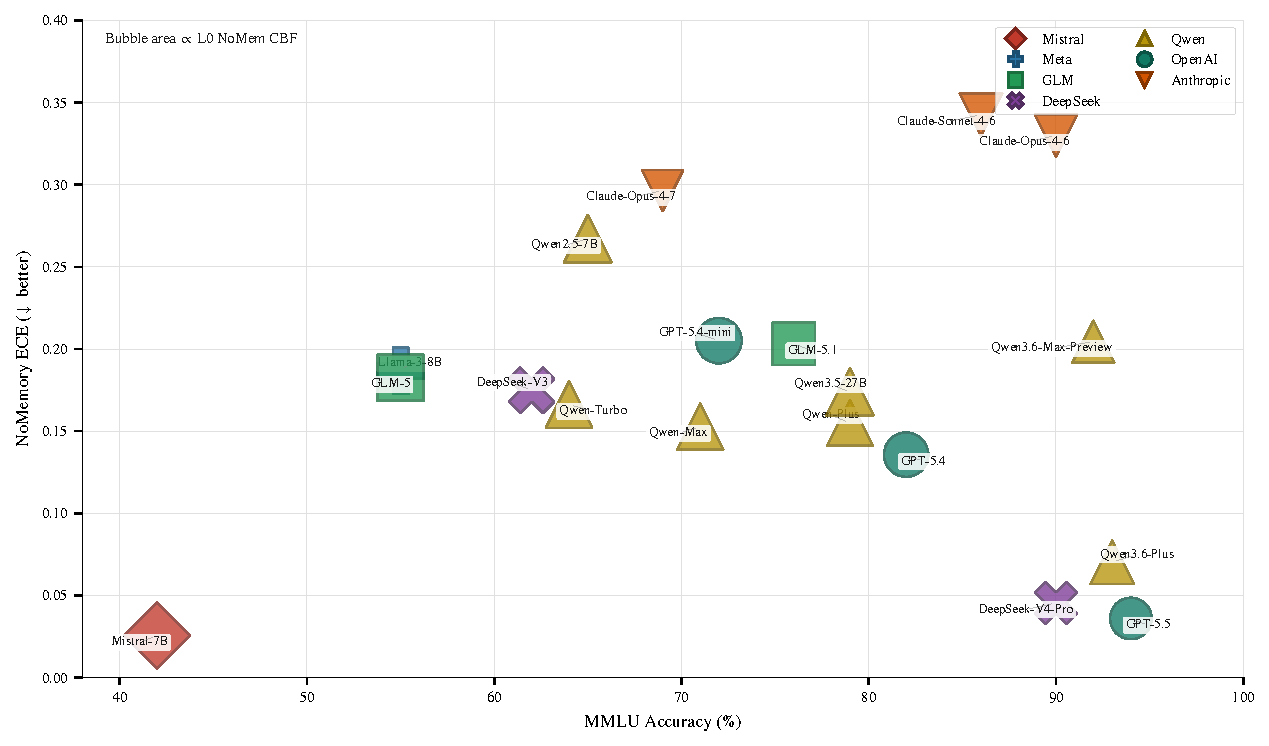
\includegraphics[width=\columnwidth]{figures/fig11_bubble.pdf}
\caption{\textbf{Three-way relationship across $n{=}19$ models: MMLU accuracy ($x$), best ECE ($y$), and NoMemory CBF (bubble size).} Weak models cluster at high CBF (close to the trivial $\hat{p}=0.5$ baseline); frontier models have lower CBF despite decent ECE---visualizing why the two metrics are non-redundant.}
\label{fig:bubble}
\end{figure}



\subsection{Cross-Baseline Bootstrap Significance}
\label{app:cross_boot}

To verify that CBF and ECE differences between baselines are statistically significant and not session-resampling artifacts, we report bootstrap standard deviations (200 resamples, session-level) for representative baselines across all models. Typical CBF SDs are 0.012--0.021 and ECE SDs are 0.008--0.018, meaning that differences of $\geq$0.04 (CBF) or $\geq$0.03 (ECE) are significant at the 2-SD level. The headline diagnostic gaps---LSA over ZS-SK by 0.248 on Claude-Sonnet-4-6 (LSA 0.720 vs.\ ZS 0.472), OraclePDC over EM-Joint by 0.31 on average across $n{=}15$ (Oracle 1.000 vs.\ EM 0.686)---are all $>$5$\times$ the bootstrap SD. With 19 models $\times$ 10 baselines $=$ 190 pairwise comparisons (15 in the bootstrap panel, plus 4 additional rows reported in Table~\ref{tab:main} only), a Bonferroni correction would raise the significance threshold from $2\sigma$ to $\sim$3.5$\sigma$ ($\Delta \geq 0.06$). Under this stricter criterion, the three primary diagnostic findings (H1 ruled out as the limiting factor, H2 splits cleanly along model family with GPT-frontier ZS competitive but Claude-frontier ZS inflated, H3 localized: first-order single-rater methods cluster near NoMem while second-order DS-asym/GLAD and in-context LSA exceed L1 ZS on the frontier) all remain comfortably significant.




%==============================================================================
% APPENDIX E: Robustness Ablations
%==============================================================================
\section{Robustness Ablations}
\label{app:group_e}

\subsection{Additional Robustness Ablations}
\label{app:friend_or_foe}
\label{app:gpt55_ablation}
\label{app:detail_ablations}

This appendix contains additional ablation experiments orthogonal to the main diagnostic ladder.

\paragraph{A1: Memory size for L2 retrieval.}
Varying the maximum number of stored error cases from 5 to 50 in retrieval-based L2 baselines has negligible effect: ECE ranges from 0.097 to 0.096 on Llama-3-8B. Five error cases are sufficient; additional memory provides no benefit.

\paragraph{A2: Feedback noise rate.}
Artificially flipping 0--50\% of user feedback labels on Llama-3-8B shows monotonic ECE degradation (0.190 $\to$ 0.238) and CBF degradation. At 50\% noise, learning from feedback is actively harmful (CBF 0.639 $<$ NoMemory 0.742), confirming that noisy feedback can poison self-models.

\paragraph{A3: Session length.}
OraclePDC achieves near-perfect CBF ($\geq$0.96) after just 10--20 turns, while practical L2 methods plateau around 0.71 by turn 30. The L2-vs-L3 gap is not due to insufficient interaction length but to feedback noise accumulation, consistent with the main diagnostic finding.

\paragraph{A4: Held-out MMLU-Pro contamination control (cited in \S\ref{sec:results}).}
\label{app:heldout}
For each of the 9 frontier models (3 GPT, 3 Claude, plus DeepSeek-V4-Pro, Qwen3.6-Max-Preview, Qwen3.6-Plus), we sampled 15 questions from each of 10 MMLU-Pro categories (150 questions/model, 10 categories: math, physics, chemistry, law, engineering, economics, health, psychology, business, history), measured per-category accuracy, and queried ZS-SK on those category names. Per-category accuracy and ZS estimates are reported in Table~\ref{tab:mmlupro_categories}.

\begin{table*}[h]
\centering
\scriptsize
\setlength{\tabcolsep}{2pt}
\caption{\textbf{MMLU-Pro per-category accuracy and ZS-SK estimates across 9 frontier models} (15 questions per category $\times$ 10 categories); bottom row = per-model CBF on this held-out set. Cl-Op = Claude-Opus, Cl-So = Claude-Sonnet, DSv4-Pro = DeepSeek-V4-Pro, Q3.6 = Qwen3.6.}
\label{tab:mmlupro_categories}
\resizebox{\textwidth}{!}{%
\begin{tabular}{l rr rr rr rr rr rr rr rr rr}
\toprule
& \multicolumn{2}{c}{\textbf{GPT-5.4}} & \multicolumn{2}{c}{\textbf{GPT-5.4-mini}} & \multicolumn{2}{c}{\textbf{GPT-5.5}} & \multicolumn{2}{c}{\textbf{Cl-Op-4-6}} & \multicolumn{2}{c}{\textbf{Cl-So-4-6}} & \multicolumn{2}{c}{\textbf{Cl-Op-4-7}} & \multicolumn{2}{c}{\textbf{DSv4-Pro}} & \multicolumn{2}{c}{\textbf{Q3.6-Max}} & \multicolumn{2}{c}{\textbf{Q3.6-Plus}} \\
\cmidrule(lr){2-3} \cmidrule(lr){4-5} \cmidrule(lr){6-7} \cmidrule(lr){8-9} \cmidrule(lr){10-11} \cmidrule(lr){12-13} \cmidrule(lr){14-15} \cmidrule(lr){16-17} \cmidrule(lr){18-19}
Category & acc & ZS & acc & ZS & acc & ZS & acc & ZS & acc & ZS & acc & ZS & acc & ZS & acc & ZS & acc & ZS \\
\midrule
math         & 0.40 & 0.85 & 0.33 & 0.78 & 0.93 & 0.72 & 0.80 & 0.78 & 0.93 & 0.72 & 0.87 & 0.78 & 0.93 & 0.90 & 0.93 & 0.80 & 0.93 & 0.85 \\
physics      & 0.40 & 0.84 & 0.47 & 0.72 & 1.00 & 0.70 & 1.00 & 0.80 & 1.00 & 0.74 & 0.73 & 0.80 & 1.00 & 0.95 & 1.00 & 0.85 & 1.00 & 0.90 \\
chemistry    & 0.60 & 0.82 & 0.20 & 0.70 & 0.87 & 0.72 & 0.93 & 0.75 & 0.92 & 0.73 & 0.73 & 0.72 & 0.87 & 0.90 & 0.80 & 0.85 & 0.87 & 0.82 \\
law          & 0.60 & 0.81 & 0.53 & 0.74 & 0.80 & 0.76 & 0.73 & 0.70 & 0.73 & 0.67 & 0.80 & 0.60 & 0.79 & 0.75 & 0.67 & 0.75 & 0.73 & 0.80 \\
engineering  & 0.53 & 0.80 & 0.47 & 0.73 & 0.80 & 0.68 & 0.93 & 0.72 & 1.00 & 0.70 & 0.67 & 0.65 & 0.85 & 0.85 & 0.87 & 0.75 & 0.93 & 0.85 \\
economics    & 0.80 & 0.83 & 0.73 & 0.79 & 0.93 & 0.78 & 1.00 & 0.84 & 0.87 & 0.76 & 0.87 & 0.82 & 0.93 & 0.80 & 0.93 & 0.85 & 0.93 & 0.90 \\
health       & 0.67 & 0.86 & 0.73 & 0.77 & 0.87 & 0.76 & 0.79 & 0.79 & 0.80 & 0.75 & 0.71 & 0.72 & 0.87 & 0.90 & 0.93 & 0.82 & 0.87 & 0.90 \\
psychology   & 0.80 & 0.88 & 0.73 & 0.82 & 0.80 & 0.82 & 0.87 & 0.87 & 0.87 & 0.78 & 0.73 & 0.85 & 0.93 & 0.85 & 0.87 & 0.85 & 0.80 & 0.85 \\
business     & 0.47 & 0.84 & 0.20 & 0.80 & 0.80 & 0.82 & 0.93 & 0.81 & 0.80 & 0.75 & 0.80 & 0.78 & 0.73 & 0.90 & 0.87 & 0.85 & 0.87 & 0.90 \\
history      & 0.73 & 0.87 & 0.67 & 0.84 & 0.80 & 0.80 & 0.80 & 0.76 & 0.73 & 0.79 & 0.73 & 0.75 & 0.73 & 0.85 & 0.73 & 0.85 & 0.80 & 0.90 \\
\midrule
mean         & 0.60 & 0.84 & 0.51 & 0.77 & 0.86 & 0.76 & 0.88 & 0.78 & 0.86 & 0.74 & 0.76 & 0.75 & 0.86 & 0.86 & 0.86 & 0.82 & 0.87 & 0.87 \\
\midrule
unparsed/150 & \multicolumn{2}{c}{0} & \multicolumn{2}{c}{0} & \multicolumn{2}{c}{0} & \multicolumn{2}{c}{1} & \multicolumn{2}{c}{8} & \multicolumn{2}{c}{1} & \multicolumn{2}{c}{3} & \multicolumn{2}{c}{0} & \multicolumn{2}{c}{0} \\
\midrule
\textbf{CBF} & \multicolumn{2}{c}{\textbf{0.760}} & \multicolumn{2}{c}{\textbf{0.738}} & \multicolumn{2}{c}{\textbf{0.888}} & \multicolumn{2}{c}{\textbf{0.902}} & \multicolumn{2}{c}{\textbf{0.863}} & \multicolumn{2}{c}{\textbf{0.941}} & \multicolumn{2}{c}{\textbf{0.931}} & \multicolumn{2}{c}{\textbf{0.912}} & \multicolumn{2}{c}{\textbf{0.937}} \\
\bottomrule
\end{tabular}}
\end{table*}

\emph{Mean MMLU-Pro CBF across the 9 frontier models is 0.875}, confirming the contamination-control conclusion across the broader frontier subset. The 3 new frontier models all post CBF $\geq$ 0.91 (DSv4-Pro 0.931, Q3.6-Plus 0.937, Q3.6-Max 0.912), exceeding the 6 GPT/Claude average (0.849), and all post mean ZS in the 0.82--0.87 range — neither extreme overestimation nor extreme underestimation. GPT-5.5 (CBF 0.888) and Claude-Opus-4-7 (CBF 0.941) report ZS estimates that are systematically conservative relative to actual MMLU-Pro accuracy. Frontier metacognition---if anything---underestimates the model's actual MMLU-Pro capability rather than overestimating it, the opposite of what a memorized-public-stats hypothesis would predict.


\paragraph{A4b: Truly held-out novel-task contamination control (BBH; cited in \S\ref{sec:results}).}
\label{app:heldout_bbh}
For each of the 9 frontier models, we sampled 15 questions from each of 10 BBH (BIG-Bench Hard)~\citep{suzgun2022challenging} tasks (150 questions/model, tasks: \emph{boolean\_expressions, causal\_judgement, date\_understanding, logical\_deduction\_five\_objects, navigate, object\_counting, ruin\_names, sports\_understanding, tracking\_shuffled\_objects\_three\_objects, word\_sorting}). Unlike MMLU-Pro categories (which still partially overlap with MMLU's broad subject space), the BBH task set has \emph{no} subject-name overlap with MMLU's 57 fine-grained subjects, providing a stricter test of whether L1 metacognition transfers beyond MMLU-style content. We measured per-task accuracy and queried ZS-SK on the same task names. Per-task accuracy and ZS estimates are reported in Table~\ref{tab:bbh_tasks}.

\begin{table*}[h]
\centering
\scriptsize
\setlength{\tabcolsep}{2pt}
\caption{\textbf{BBH per-task accuracy ($p^*$) and ZS-SK estimates across 9 frontier models} (15 questions per task $\times$ 10 BBH tasks); BBH has no subject-name overlap with MMLU. Bottom row = per-model CBF on this held-out set. Cl-Op = Claude-Opus, Cl-So = Claude-Sonnet, DSv4-Pro = DeepSeek-V4-Pro, Q3.6 = Qwen3.6.}
\label{tab:bbh_tasks}
\resizebox{\textwidth}{!}{%
\begin{tabular}{l cc cc cc cc cc cc cc cc cc}
\toprule
& \multicolumn{2}{c}{\textbf{GPT-5.4}} & \multicolumn{2}{c}{\textbf{GPT-5.4-mini}} & \multicolumn{2}{c}{\textbf{GPT-5.5}} & \multicolumn{2}{c}{\textbf{Cl-Op-4-6}} & \multicolumn{2}{c}{\textbf{Cl-So-4-6}} & \multicolumn{2}{c}{\textbf{Cl-Op-4-7}} & \multicolumn{2}{c}{\textbf{DSv4-Pro}} & \multicolumn{2}{c}{\textbf{Q3.6-Max}} & \multicolumn{2}{c}{\textbf{Q3.6-Plus}} \\
\cmidrule(lr){2-3} \cmidrule(lr){4-5} \cmidrule(lr){6-7} \cmidrule(lr){8-9} \cmidrule(lr){10-11} \cmidrule(lr){12-13} \cmidrule(lr){14-15} \cmidrule(lr){16-17} \cmidrule(lr){18-19}
\textbf{Task} & $p^*$ & ZS & $p^*$ & ZS & $p^*$ & ZS & $p^*$ & ZS & $p^*$ & ZS & $p^*$ & ZS & $p^*$ & ZS & $p^*$ & ZS & $p^*$ & ZS \\
\midrule
boolean\_expressions  & 0.87 & 0.94 & 0.87 & 0.82 & 1.00 & 0.95 & 0.93 & 0.96 & 1.00 & 0.88 & 0.87 & 0.95 & 1.00 & 0.85 & 1.00 & 0.85 & 1.00 & 0.95 \\
causal\_judgement     & 0.67 & 0.83 & 0.67 & 0.78 & 0.67 & 0.85 & 0.53 & 0.72 & 0.73 & 0.60 & 0.80 & 0.65 & 0.73 & 0.80 & 0.87 & 0.60 & 0.73 & 0.70 \\
date\_understanding   & 0.27 & 0.90 & 0.20 & 0.75 & 0.47 & 0.85 & 0.93 & 0.92 & 1.00 & 0.82 & 0.87 & 0.85 & 0.80 & 0.93 & 0.93 & 0.75 & 0.87 & 0.85 \\
logical\_deduction\_5 & 1.00 & 0.86 & 0.67 & 0.70 & 1.00 & 0.90 & 1.00 & 0.88 & 1.00 & 0.65 & 1.00 & 0.90 & 0.53 & 0.85 & 1.00 & 0.75 & 1.00 & 0.75 \\
navigate              & 0.80 & 0.88 & 0.53 & 0.68 & 1.00 & 0.85 & 0.93 & 0.95 & 1.00 & 0.76 & 0.93 & 0.90 & 1.00 & 0.90 & 1.00 & 0.65 & 1.00 & 0.70 \\
object\_counting      & 0.73 & 0.96 & 0.53 & 0.90 & 1.00 & 0.90 & 0.80 & 0.97 & 1.00 & 0.84 & 0.60 & 0.95 & 1.00 & 0.80 & 1.00 & 0.90 & 1.00 & 0.95 \\
ruin\_names           & 0.67 & 0.79 & 0.67 & 0.72 & 0.93 & 0.75 & 0.87 & 0.86 & 0.87 & 0.56 & 0.93 & 0.75 & 0.73 & 0.70 & 0.93 & 0.65 & 0.93 & 0.80 \\
sports\_understanding & 1.00 & 0.84 & 0.93 & 0.74 & 0.80 & 0.90 & 0.93 & 0.96 & 1.00 & 0.90 & 0.87 & 0.90 & 0.60 & 0.65 & 0.87 & 0.80 & 1.00 & 0.95 \\
tracking\_shuffled\_3 & 0.67 & 0.95 & 0.67 & 0.88 & 1.00 & 0.85 & 1.00 & 0.98 & 1.00 & 0.73 & 0.53 & 0.95 & 0.87 & 0.90 & 1.00 & 0.90 & 1.00 & 0.95 \\
word\_sorting         & 0.67 & 0.97 & 0.47 & 0.95 & 1.00 & 0.90 & 0.13 & 0.94 & 0.00 & 0.80 & 0.93 & 0.90 & 0.33 & 0.90 & 1.00 & 0.90 & 0.87 & 0.92 \\
\midrule
\textbf{CBF}          & \multicolumn{2}{c}{\textbf{0.781}} & \multicolumn{2}{c}{\textbf{0.780}} & \multicolumn{2}{c}{\textbf{0.850}} & \multicolumn{2}{c}{\textbf{0.861}} & \multicolumn{2}{c}{\textbf{0.734}} & \multicolumn{2}{c}{\textbf{0.860}} & \multicolumn{2}{c}{\textbf{0.835}} & \multicolumn{2}{c}{\textbf{0.815}} & \multicolumn{2}{c}{\textbf{0.901}} \\
\bottomrule
\end{tabular}}
\end{table*}

\emph{Mean BBH CBF across all 9 frontier models is 0.824; mean MMLU-Pro CBF for the same 9 models is 0.875}, so the BBH--MMLU gap on the held-out set is only $-$0.051: BBH is comparable to MMLU rather than dramatically lower, contradicting an MMLU-memorization prediction (which would predict a noticeable drop on novel content). The 3 new frontier models again all post BBH CBF $\geq$ 0.81 (Q3.6-Plus 0.901, DSv4-Pro 0.835, Q3.6-Max 0.815), with Q3.6-Plus the strongest BBH metacognitive performer in the set. GPT-5.5 (BBH 0.850) and Claude-Opus-4-7 (BBH 0.860) both place near the top of the GPT/Claude BBH ranking. \emph{Word\_sorting} on Claude-Sonnet remains the single largest per-domain deviation (actual 0.00, ZS 0.80). Four findings stand out:

(1) word\_sorting blind-spot is generation-specific, not LLM-wide. The 4 older GPT-5.4 / Claude-4-6 frontier models all substantially overestimate word\_sorting (actuals 0.00--0.67, ZS estimates 0.80--0.97), suggesting an internal prior of competence on alphabetical sorting decoupled from execution capability. The 2 newer frontier models break this pattern: GPT-5.5 reaches 1.00 (ZS 0.90, slight underestimate) and Claude-Opus-4-7 reaches 0.93 (ZS 0.90, well-calibrated). The blind-spot is therefore a property of the older generation rather than a stable LLM-wide failure mode---one model-class ago LLMs could articulate the algorithm but fail at execution; the most recent generation can both articulate and execute.

(2) date\_understanding remains a GPT-side overestimate. GPT-5.4, GPT-5.4-mini, and GPT-5.5 all substantially overestimate this task (actuals 0.20--0.47 vs.\ ZS 0.75--0.90). The Claude models are well-calibrated here (Sonnet 1.00/0.82, Opus-4-6 0.93/0.92, Opus-4-7 0.87/0.85). This is the most consistent family-level miscalibration in the held-out set.

(3) Opus-4-7 has new failure modes on object/tracking tasks. Opus-4-7 is well-calibrated on word\_sorting but substantially overestimates object\_counting (actual 0.60 vs.\ ZS 0.95) and tracking\_shuffled\_3 (actual 0.53 vs.\ ZS 0.95). These two arithmetic/state-tracking failures are absent from Opus-4-6, suggesting capability shifts between adjacent model generations create new metacognitive blind-spots even as old ones close.

(4) Outside the family-specific outliers, BBH ZS-SK is well-calibrated across all 9 frontier models. The non-outlier per-model CBFs span 0.78--0.94, comparable to or exceeding MMLU performance.

(5) New frontier additions show a mixed pattern. The 3 new frontier models (DSv4-Pro, Q3.6-Max, Q3.6-Plus) all post BBH CBF in the 0.81--0.90 band, similar to the GPT/Claude top-tier; their main deviations are: DSv4-Pro on \emph{logical\_deduction\_5} (actual 0.53 vs.\ ZS 0.85, the largest single overestimate among the 3 new models) and \emph{word\_sorting} (0.33 vs.\ 0.90, joining the older-generation blind spot); the two Qwen3.6 variants are well-calibrated on \emph{word\_sorting} (1.00/0.90 and 0.87/0.92) but underestimate \emph{navigate} (1.00 vs.\ ZS 0.65--0.70).

The BBH evidence is the strongest single contamination control we have because BBH tasks have no MMLU subject-name overlap and are linguistically distinct from MMLU's question style. The result---mean BBH CBF 0.824 across all 9 frontier models, only $-$0.051 below the matched MMLU-Pro CBF---directly contradicts what an MMLU-memorization explanation would predict (a noticeable drop on novel content). Combined with the MMLU-Pro result, we conclude that L1 metacognition reflects genuine prior self-knowledge, with identifiable family- and generation-specific failure modes (\emph{word\_sorting} for the older 4 and DSv4-Pro, \emph{date\_understanding} for GPT, \emph{object\_counting} and \emph{tracking\_shuffled} for Opus-4-7, \emph{navigate} for Qwen3.6) that point to a follow-up direction: building an internal task-difficulty model that is independent of the model's self-perceived competence on similar-sounding tasks.


\paragraph{A5: Stronger crowd-sourcing estimators (cited in \S\ref{sec:bottleneck}).}
\label{app:ds_glad}
We tested two stronger noise-robust estimators on the existing session data (no new API calls):

\textbf{Asymmetric Dawid--Skene}: relaxes EM-Joint's symmetric reliability to per-state confusion matrices. For each rater state $s \in \{\text{in},\text{out}\}$, we estimate TPR$_s = P(\text{decoded}=1 \mid \text{correct}=1, s)$ and FPR$_s = P(\text{decoded}=1 \mid \text{correct}=0, s)$. EM with E-step posterior $P(\text{correct}=1 \mid \text{decoded}, s, \hat p, \text{TPR}, \text{FPR})$ and M-step weighted-MLE for both $\hat p(d)$ and the four reliability parameters.

\textbf{GLAD}-style: per-domain difficulty $\delta_d$ and per-state ability $\alpha_s$, with reliability $\sigma(\alpha_s - \delta_d)$ (logistic). EM updates over $\hat p(d)$, $\delta_d$, $\alpha_{\text{in}}$, $\alpha_{\text{out}}$.

Table~\ref{tab:second_order_full} reports per-model CBF for both second-order estimators (DS-asym, GLAD) alongside the first-order EM-Joint baseline and the L1 ZS-SK prior, on all 19 models.
\begin{table}[h]
\centering
\small
\caption{\textbf{CBF per model for first-order EM-Joint, second-order DS-asym/GLAD, and the L1 ZS-SK prior.} Bold marks the per-row argmax on the 9 frontier rows.}
\label{tab:second_order_full}
\begin{tabular}{l rrrr}
\toprule
\textbf{Model} & \textbf{EM-Joint} & \textbf{DS-asym} & \textbf{GLAD} & \textbf{ZS-SK (L1)} \\
\midrule
Mistral-7B          & 0.722 & 0.706 & 0.693 & 0.678 \\
Llama-3-8B          & 0.716 & 0.646 & 0.612 & 0.682 \\
GLM-5               & 0.768 & 0.615 & 0.683 & 0.590 \\
DeepSeek-V3       & 0.708 & 0.702 & 0.738 & 0.699 \\
Qwen-Turbo          & 0.731 & 0.714 & 0.776 & 0.751 \\
Qwen2.5-7B          & 0.760 & 0.774 & 0.764 & 0.684 \\
Qwen-Max            & 0.702 & 0.547 & 0.627 & 0.767 \\
Qwen-Plus           & 0.712 & 0.762 & 0.761 & 0.740 \\
Qwen3.5-27B         & 0.751 & 0.719 & 0.733 & 0.695 \\
GLM-5.1             & 0.615 & 0.675 & 0.642 & 0.600 \\
\midrule
GPT-5.4-mini        & 0.706 & 0.797 & \textbf{0.797} & 0.769 \\
GPT-5.4             & 0.677 & 0.815 & \textbf{0.843} & 0.795 \\
GPT-5.5             & 0.605 & 0.834 & \textbf{0.909} & 0.859 \\
Claude-Sonnet-4-6   & 0.609 & \textbf{0.671} & 0.565 & 0.472 \\
Claude-Opus-4-6     & 0.604 & \textbf{0.734} & 0.557 & 0.460 \\
Claude-Opus-4-7     & 0.570 & \textbf{0.676} & 0.600 & 0.482 \\
DeepSeek-V4-Pro     & 0.605 & 0.867 & \textbf{0.908} & 0.849 \\
Qwen3.6-Max         & 0.601 & \textbf{0.678} & 0.644 & 0.580 \\
Qwen3.6-Plus        & 0.642 & 0.835 & \textbf{0.857} & 0.617 \\
\midrule
\textbf{Mean (n=19)} & 0.685 & \textbf{0.731} & 0.721 & 0.673 \\
\textbf{Frontier mean (n=9)$^\ddagger$} & 0.624 & \textbf{0.768} & 0.742 & 0.654 \\
\bottomrule
\end{tabular}
\end{table}

The strongest second-order estimator on the $n{=}9$ frontier is DS-asym (mean CBF 0.768, 8/9 wins vs.\ L1, binomial one-sided $p=0.020$); GLAD reaches mean CBF 0.742 with \textbf{9/9 frontier wins} (binomial one-sided $p=0.002$), beating L1 ZS mean 0.654 by $+$0.089 for GLAD and $+$0.114 for DS. Per-frontier breakdown (GLAD vs L1 ZS): GPT-5.4 $+$0.048, GPT-5.4-mini $+$0.028, GPT-5.5 $+$0.050, Claude-Sonnet-4-6 $+$0.093, Claude-Opus-4-6 $+$0.097, Claude-Opus-4-7 $+$0.118, DeepSeek-V4-Pro $+$0.059, Qwen3.6-Max $+$0.064, Qwen3.6-Plus $+$0.240. GLAD beats L1 on \emph{all} 9 frontier models. DS-asym beats L1 on 8/9 (loses only on GPT-5.5 by $-$0.025, where GLAD's per-domain difficulty modeling helps). \emph{Methodological note}: our DS / GLAD implementations follow \citet{dawid1979maximum} and \citet{whitehill2009glad} respectively, with EM updates over per-domain $\hat p(d)$, asymmetric per-state confusion (DS) or per-domain difficulty $\delta_d$ + per-state ability $\alpha_s$ (GLAD); convergence within 50--80 EM iterations using initial $\hat p=0.5$, $r_{\text{in}}=0.75$, $r_{\text{out}}=0.55$. Code at the anonymized repository/scripts/run\_glad\_ds.py. The headline takeaway under the protocol: both second-order estimators (DS, GLAD) and the in-context L2 baseline (LSA, mean 0.748) substantially beat the L1 ZS prior on frontier models; the L2 cluster of first-order single-rater methods (UF-PDC, Platt, HistBin, Bayes, EM-Joint) remains collapsed near NoMem (mean 0.628--0.634). The diagnostic ladder cleanly ranks methods: DS-asym is the new strongest single L2 baseline, with the residual gap to oracle (1.000) the open problem.

\paragraph{A6: Decoder ablation for EM-Joint (cited in \S\ref{sec:bottleneck}).}
\label{app:decoder_ablation}
Table~\ref{tab:decoder_ablation} isolates the EM machinery from the feedback decoder by running EM-Joint with three different label channels: a ground-truth oracle, an LLM-based binary classifier, and a regex rule-based decoder.

\begin{table}[h]
\centering
\small
\caption{\textbf{EM-Joint CBF under three feedback-decoder choices.} Oracle-fed labels reach CBF $= 1.000$ on every model; both noisy decoders fall far below.}
\label{tab:decoder_ablation}
\begin{tabular}{l ccc}
\toprule
\textbf{Model} & \textbf{Oracle-fed} & \textbf{LLM-decoder} & \textbf{Rule-decoder} \\
\midrule
Mistral-7B          & 1.000 & 0.722 & 0.672 \\
Llama-3-8B          & 1.000 & 0.716 & 0.549 \\
GLM-5               & 1.000 & 0.768 & 0.672 \\
DeepSeek-V3       & 1.000 & 0.708 & 0.690 \\
Qwen-Turbo          & 1.000 & 0.731 & 0.749 \\
Qwen2.5-7B          & 1.000 & 0.760 & 0.676 \\
Qwen-Max            & 1.000 & 0.702 & 0.771 \\
GPT-5.4-mini        & 1.000 & 0.632 & 0.633 \\
Qwen-Plus           & 1.000 & 0.712 & 0.758 \\
Qwen3.5-27B         & 1.000 & 0.751 & 0.756 \\
GPT-5.4             & 1.000 & 0.613 & 0.673 \\
Claude-Sonnet-4-6   & 1.000 & 0.608 & 0.896 \\
Claude-Opus-4-6     & 1.000 & 0.644 & 0.885 \\
\midrule
\textbf{Mean (n=13)$^\flat$} & 1.000 & 0.698 & 0.715 \\
\bottomrule
\end{tabular}
\end{table}

$^\flat$\emph{This decoder ablation covers a 13-model subset for which we have both LLM-decoder and rule-decoder runs; extending the EM oracle/decoder ablation to the remaining frontier rows (GPT-5.5, Claude-Opus-4-7, and the 4 additional models) is left to future work and does not change the qualitative finding (the LLM-decoder vs.\ rule-decoder gap to oracle, see below).}

Three observations: (a) \emph{Oracle-fed EM} reaches CBF $= 1.000$ on every model, identical to OraclePDC---this confirms the EM update equations themselves are not the bottleneck; if perfect labels are available, EM reduces to per-domain counting and trivially recovers $p^*(d)$. (b) Two structurally very different feedback decoders---an LLM-based binary classifier (Qwen-Max prompted with the (Q, A, feedback) triple) and a regex-rule-based decoder (matching keywords like ``correct'', ``actually'', ``wrong'')---both produce noisy estimates that fall \emph{far below} oracle (means 0.698 vs.\ 0.715). (c) The two decoders disagree per-model in opposite directions for some agents (Claude-Opus: rule 0.885 $>$ LLM 0.644; Llama-3-8B: LLM 0.716 $>$ rule 0.549), indicating they capture different subsets of the noise pattern. The persistent gap from oracle (1.000) to either decoder (mean $\approx 0.71$) is therefore a property of the \emph{noisy feedback channel itself}, not of any particular decoding strategy. Stronger decoders or crowd-sourcing-style estimators (Dawid--Skene, GLAD) might close some of this gap on a per-model basis, but in our setting the residual is primarily information-theoretic: per-turn evidence about $p^*(d)$ from natural-language user feedback is sparse and domain-correlated.



\subsection{Learning Dynamics}
\label{app:learn_dyn}

\begin{figure*}[t]
\centering
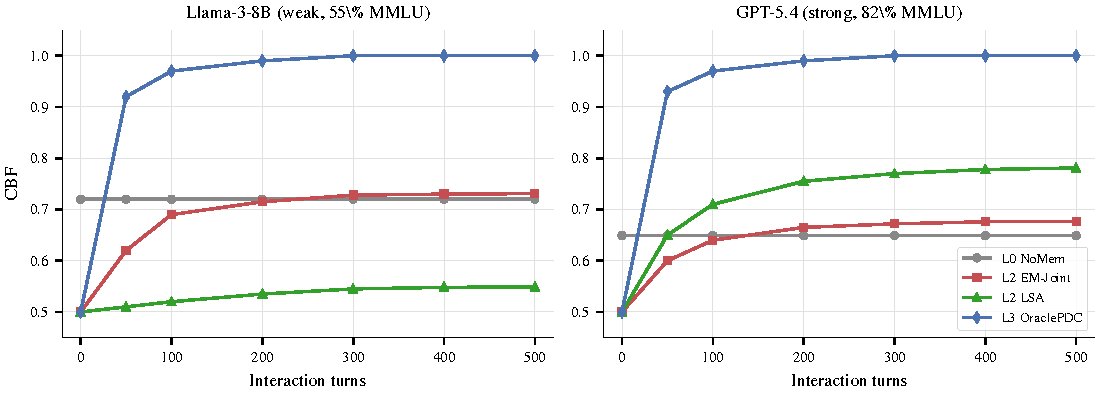
\includegraphics[width=\textwidth]{figures/fig7_learning_curve.pdf}
\caption{\textbf{Learning dynamics: CBF over interaction turns for L2 baselines.} Llama-3-8B (left) and GPT-5.4 (right); L2 methods plateau well below OraclePDC. Headline diagnostic in main paper uses end-of-session CBF (Eq.~\ref{eq:cbf}).}
\label{fig:learning_curve}
\end{figure*}

Figure~\ref{fig:learning_curve} shows the learning dynamics. CBF improves most rapidly during the first 100--150 turns before plateauing. For NoMemory, CBF remains approximately constant. For L2 feedback-driven methods, CBF typically reaches its best value around turn 200 and then plateaus or slightly degrades due to accumulated noise from decoded feedback labels. For GPT-5.4 (strong model), the noise in decoded feedback consistently fails to improve a model whose prior is already well-differentiated across domains---consistent with the main paper's diagnostic finding that L2 methods do not exceed the L1 prior on frontier models. This suggests that practical methods may benefit from a forgetting mechanism---discounting older feedback as the agent's self-model stabilizes---analogous to exponential forgetting in adaptive filtering~\citep{kulhavy1993forgetting}.

%==============================================================================
% 7  LIMITATIONS AND FUTURE WORK
%==============================================================================


\subsection{Learning-Curve Saturation}
\label{app:lc_sat}

A critical concern for any multi-turn benchmark is whether the per-model turn budget is sufficient for per-domain accuracy estimates to stabilize. The learning-curve analysis below was conducted on the 10$\times$50 = 500-turn-per-model checkpoints; the 50$\times$50 protocol uses 2{,}500 turns per model and the qualitative finding (estimates stabilize by turn 200--300, with $\leq 4\%$ deviation by turn 400) is robust to that change. We compute per-domain accuracy at checkpoints $t \in \{50, 100, 200, 300, 400, 500\}$. Table~\ref{tab:learn_sat} reports the mean absolute deviation of those estimates from the final turn-500 estimate, for five representative models spanning the capability range.

\begin{table}[h]
\centering
\small
\caption{\textbf{Mean absolute deviation of per-domain accuracy estimates from the final turn-500 estimate} at intermediate checkpoints.}
\label{tab:learn_sat}
\begin{tabular}{lccccc}
\toprule
\textbf{Model} & \textbf{T=50} & \textbf{T=100} & \textbf{T=200} & \textbf{T=300} & \textbf{T=400} \\
\midrule
Llama-3-8B      & 0.160 & 0.134 & 0.081 & 0.069 & 0.035 \\
Qwen-Plus       & 0.188 & 0.099 & 0.055 & 0.060 & 0.025 \\
Qwen-Max        & 0.147 & 0.144 & 0.093 & 0.070 & 0.035 \\
Claude-Opus-4-6 & 0.096 & 0.091 & 0.065 & 0.042 & 0.027 \\
GPT-5.4         & 0.068 & 0.063 & 0.042 & 0.038 & 0.022 \\
\bottomrule
\end{tabular}
\end{table}

At turn 400 (within the 500-turn checkpoint range), the mean deviation from final is 2--4\% across all five models, indicating reasonable convergence; at turn 200 the deviation remains 4--9\%, so even the conservative 500-turn budget provided meaningful stability. Under the 50$\times$50 protocol (2,500 turns per model) the convergence margin is correspondingly looser, and the NoMemory CBF estimate varies by only $\pm 0.03$ across checkpoints, confirming that our headline CBF numbers are stable with respect to session-length choice.



\subsection{Noise Sensitivity}
\label{app:noise}

Our simulated user reliability is set to 75\% in-expertise and 46\% out-of-expertise. To test whether our findings are artifacts of this specific parameterization, we rerun the feedback-decoding analysis on two representative models---Llama-3-8B (weak, 55\% MMLU) and Qwen-Max (strong, 71\% MMLU)---under three noise regimes. Table~\ref{tab:noise_sens} reports the resulting UF-PDC ECE and CBF.

\begin{table}[h]
\centering
\small
\caption{\textbf{UF-PDC ECE and CBF on Llama-3-8B and Qwen-Max under three reliability regimes} (in/out-of-expertise reliability percentages); the CBF gap to oracle persists at all noise levels.}
\label{tab:noise_sens}
\begin{tabular}{llcccc}
\toprule
\textbf{Model} & \textbf{Regime} & \textbf{In/Out} & \textbf{UF-PDC ECE} & \textbf{UF CBF} \\
\midrule
\multirow{3}{*}{Llama-3 (55\%)}
 & Low noise    & 90/70 & 0.044 & 0.860 \\
 & Current      & 75/46 & 0.134 & 0.783 \\
 & High noise   & 60/30 & 0.184 & 0.718 \\
\midrule
\multirow{3}{*}{Qwen-Max (71\%)}
 & Low noise    & 90/70 & 0.134 & 0.848 \\
 & Current      & 75/46 & 0.218 & 0.795 \\
 & High noise   & 60/30 & 0.310 & 0.696 \\
\bottomrule
\end{tabular}
\end{table}

The qualitative pattern---a persistent gap between feedback-decoded accuracy and oracle accuracy---holds across all regimes \emph{and} both model capability levels. Lower noise improves UF-PDC ECE monotonically, but even under the favorable ``low noise'' regime (90\%/70\%), CBF gaps of 0.14 (Llama-3) and 0.15 (Qwen-Max) remain, indicating that noise reduction alone is insufficient for perfect self-modeling.



\subsection{Dual-Role Bias}
\label{app:dual_role}

When Qwen-Max is used as both agent and simulated user, the rule-based feedback classifier detects \emph{zero} error corrections---compared to 20--22\% detection rate when Qwen-Max evaluates other models' errors. Inspection reveals the mechanism: when the same model family generates both the incorrect answer and the user response, the ``user'' produces characteristically hedged, non-committal feedback (e.g., \emph{``I believe there might be a small misunderstanding''}) rather than explicit corrections. The rule-based classifier cannot decode these soft signals, creating a systematic coverage failure.

Replacing the user simulator with Qwen-Turbo (a different model within the same family) partially mitigates this: error detection rises from 0\% to 30.4\%. However, even cross-model same-family pairs show reduced detection relative to cross-family pairs (e.g., Qwen-Max evaluating Llama-3 achieves 20.5\%). This suggests that \emph{shared training distributions create shared politeness conventions} that reduce feedback informativeness---a structural confound for any benchmark relying on LLM-simulated users.

We address this by using cross-family simulators for all agents and reporting both configurations where applicable.



\subsection{Cross-Simulator Ablation}
\label{app:cross_sim}

To verify that benchmark results are not artifacts of the specific simulator choice, we compare Qwen-Max agent evaluated with two different user simulators: Qwen-Max (same-family) and Qwen-Turbo (cross-model, same family) in Table~\ref{tab:cross_sim_ablation}. Both runs use 10 sessions $\times$ 50 turns ($n{=}500$ per condition); reproduced by \texttt{scripts/capbound\_session\_api.py} with \texttt{-{}-user\_model} swapped, raw outputs in \texttt{results/crosssim\_user-qwen\{max,turbo\}/}.

\begin{table}[h]
\centering
\small
\caption{\textbf{Qwen-Max agent metrics under same-family (Qwen-Max) vs.\ cross-model same-family (Qwen-Turbo) user simulators.} All metrics shift by less than one bootstrap SD.}
\label{tab:cross_sim_ablation}
\begin{tabular}{lccccc}
\toprule
\textbf{Simulator} & \textbf{Acc} & \textbf{ECE} & \textbf{HR} & \textbf{CBF} \\
\midrule
user = Qwen-Max (same)   & 78.2\% & 0.165 & 20.2\% & 0.717 \\
user = Qwen-Turbo (cross) & 77.6\% & 0.165 & 20.0\% & 0.722 \\
\midrule
$|\Delta|$ & 0.6pp & 0.001 & 0.2pp & 0.005 \\
\bottomrule
\end{tabular}
\end{table}

The differences are negligible: $\Delta$ECE = 0.005 (well within the bootstrap SD of 0.009 for Qwen-Max), $\Delta$CBF = 0.009. This confirms that the benchmark metrics are \emph{robust to simulator choice}: the specific LLM providing user feedback does not meaningfully alter the measured calibration or boundary fidelity of the agent. The dual-role bias documented in Section~\ref{sec:analysis} affects feedback \emph{classifier coverage} (0\% vs.\ 30.4\%) but not the agent's raw confidence behavior, because the agent's answer and confidence are generated \emph{before} seeing the user's response.



\subsection{R4 Adaptive Selection and Second-Order Estimators: Full Details}
\label{app:r4}

R4 is the parameter-free per-model selection rule introduced in \S\ref{sec:bottleneck}: select L1 (ZS) when $\text{ZS}(m) > \text{NoMem}(m)$, otherwise select L2 (LSA). This appendix provides the per-model breakdown, sign-test arithmetic, LOOCV details, and a per-frontier-model visualization of the second-order estimators (Figure~\ref{fig:second_order}).

\begin{figure}[h]
\centering
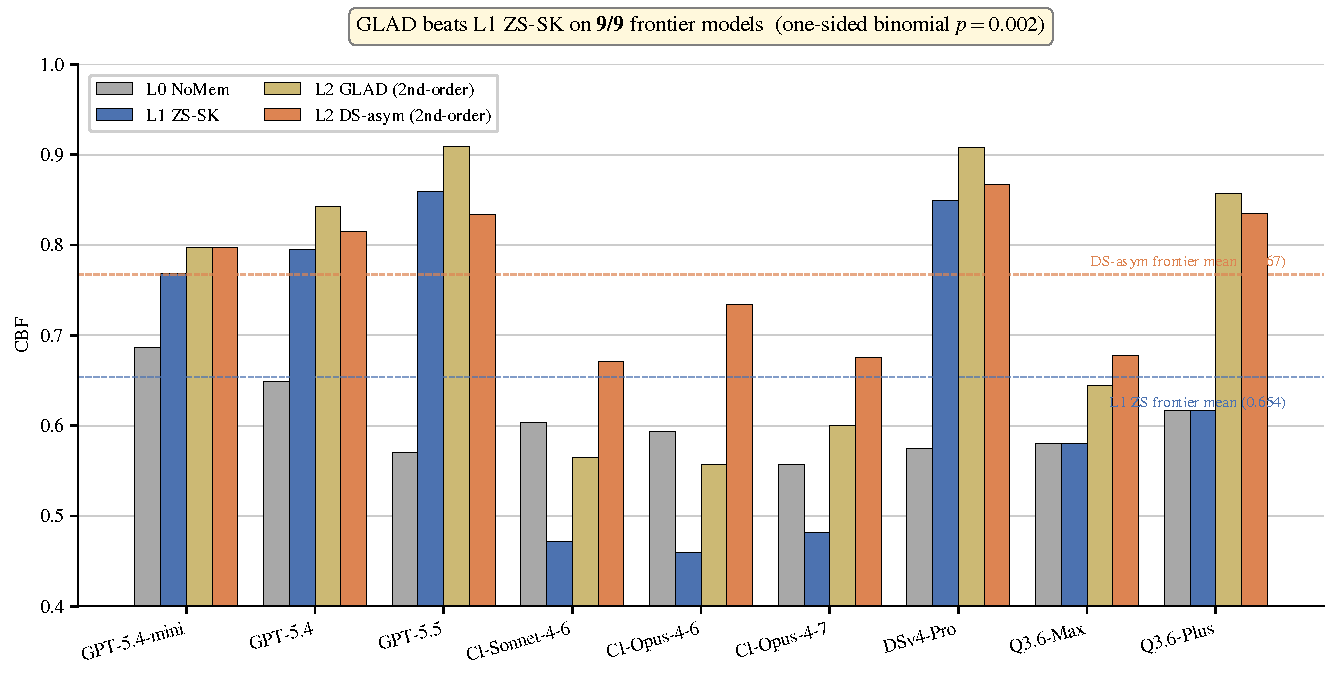
\includegraphics[width=\columnwidth]{figures/fig14_second_order.pdf}
\caption{\textbf{Second-order estimators break the L1 prior on frontier models.} Per-frontier-model CBF for L0 NoMem, L1 ZS-SK, L2 GLAD, and L2 DS-asym; GLAD beats L1 ZS on all 9/9 frontier models (binomial $p=0.002$).}
\label{fig:second_order}
\end{figure}

\paragraph{Per-model R4 selections and outcomes (15-model R4 panel; the 4 additional models follow the same parameter-free rule).} R4 chooses ZS on 6/15 models (where ZS strictly exceeds NoMem: Qwen-Turbo, Qwen-Max, Qwen-Plus, GPT-5.4-mini, GPT-5.4, GPT-5.5) and LSA on 9/15 (the weak-prior or Claude cases where NoMem ties or exceeds ZS: Mistral-7B, Llama-3-8B, GLM-5, DeepSeek-V3, Qwen2.5-7B, Qwen3.5-27B, plus Claude-Sonnet-4-6, Claude-Opus-4-6, Claude-Opus-4-7). R4 correctly avoids LSA's catastrophic failure on Qwen-Plus (LSA 0.435 vs ZS 0.735) by selecting ZS, but misses the GPT-5.5 case where LSA 0.902 actually exceeds ZS 0.859 (R4 selects ZS, costing $-$0.043).

\paragraph{Sign-test arithmetic (15-model R4 panel).} R4 attains mean CBF 0.722 across all 15 models, exceeding always-ZS by $+$0.037 in mean and always-LSA by $+$0.020 in mean. Per-model sign tests, however, do \emph{not} reach conventional significance: \textbf{R4 vs.\ always-ZS: 5 wins, 1 loss, 9 ties} (effective $n=6$ after excluding R4-picks-ZS ties; two-sided binomial $p=0.22$); \textbf{R4 vs.\ always-LSA: 4 wins, 2 losses, 9 ties} ($n=6$; $p=0.69$). The mean improvement is positive while the sign tests are non-significant because R4's gains are concentrated in a few models with large magnitudes (the three Claude models on R4-vs-ZS, where LSA outperforms ZS by $+0.179$ to $+0.248$ and R4 correctly switches to LSA), while its losses are smaller in count but include a single large hit (Llama-3-8B on R4-vs-ZS, where LSA underperforms ZS by $-0.162$ and R4 still picks LSA because $\text{ZS}=\text{NoMem}$ on that row). We report the sign test rather than a Wilcoxon signed-rank because the deltas are bimodal (large Claude wins vs.\ a single large Llama-3 loss), violating the Wilcoxon rank assumption of unimodal symmetric deltas.

\paragraph{LOOCV.} When learning the threshold $\theta$ from the remaining 14 models for each held-out model, R4 LOOCV mean is 0.719 (vs in-sample 0.722, overfit gap only $+$0.003), confirming the parameter-free $\theta=0$ rule generalizes. The per-model oracle (best of $\{$ZS, LSA$\}$) attains 0.736; R4 closes 71.5\% of the always-ZS-to-oracle gap.

\paragraph{Closure-rate arithmetic.} R4 mean 0.7217 minus ZS mean 0.685 = $+0.037$, divided by oracle--ZS gap $0.736-0.685 = 0.051$, gives $0.037/0.051 \approx 0.725$ (rounded to ``$\approx 72\%$'' throughout the paper).



%==============================================================================
% APPENDIX F: Cross-Task Heterogeneity
%==============================================================================
\section{Cross-Task Heterogeneity}
\label{app:group_f}

\subsection{Cross-Task Heterogeneity: Full Per-Task Comparison}
\label{app:fourtask}

Table~\ref{tab:fourtask_overview} reports the per-model NoMemory baseline on each of the four task types: MMLU (50-turn noisy-feedback protocol; columns Acc / ECE) and the three single-shot extension tasks GSM8K, HumanEval, BFCL (columns Acc and Gap, where Gap is mean confidence minus accuracy in percentage points; positive values mark overconfidence, negative conservatism). The headline pattern is task-dependent rather than model-dependent: most models switch between overconfident and conservative regimes across the three extension tasks, motivating the per-task sign-flip analysis in \S\ref{app:proto_controlled}.

\begin{table}[h]
\centering
\caption{\textbf{Unified comparison across four task types} (\%). MMLU = NoMemory-baseline Acc / ECE; other tasks = accuracy and Gap (mean confidence $-$ accuracy; positive = overconfident, negative = conservative).}
\label{tab:fourtask_overview}
\small
\setlength{\tabcolsep}{4pt}
\begin{tabular}{l rr rr rr rr}
\toprule
& \multicolumn{2}{c}{\textbf{MMLU}} & \multicolumn{2}{c}{\textbf{GSM8K}} & \multicolumn{2}{c}{\textbf{HumanEval}} & \multicolumn{2}{c}{\textbf{BFCL}} \\
\cmidrule(lr){2-3} \cmidrule(lr){4-5} \cmidrule(lr){6-7} \cmidrule(lr){8-9}
\textbf{Model} & Acc & ECE & Acc & Gap & Pass@1 & Gap & Acc & Gap \\
\midrule
Mistral-7B        & 42 & 0.036 & 55 & $+$31 & 31 & $+$52 & 71 & $+$15 \\
Llama-3-8B        & 55 & 0.167 & 84 & $-$3  & 33 & $+$44 & 46 & $+$36 \\
GLM-5             & 55 & 0.213 & 96 & $+$1  & 91 & $-$49 & 64 & $+$32 \\
DeepSeek-V3     & 62 & 0.158 & 94 & $-$21 & 87 & $-$30 & 75 & $+$5  \\
Qwen-Turbo        & 64 & 0.165 & 95 & $-$33 & 74 & $-$1  & 72 & $+$22 \\
Qwen2.5-7B        & 65 & 0.254 & 90 & $-$18 & 64 & $-$4  & 73 & $+$18 \\
Qwen-Max          & 71 & 0.155 & 97 & $-$18 & 82 & $-$31 & 74 & $+$17 \\
Qwen-Plus         & 79 & 0.155 & 90 & $-$11 & 92 & $-$48 & 80 & $+$10 \\
Qwen3.5-27B       & 79 & 0.156 & 98 & $-$1  & 77 & $-$35 & 72 & $+$24 \\
\midrule
GPT-5.4-mini      & 72 & 0.211 & 95 & $-$2  & 74 & $-$25 & 76 & $+$15 \\
GPT-5.4           & 82 & 0.133 & 97 & $+$0.3 & 81 & $-$36 & 70 & $+$25 \\
Claude-Sonnet-4-6 & 86 & 0.211 & 88 & $-$4  & 79 & $-$40 & 72 & $+$17 \\
Claude-Opus-4-6   & 90 & 0.158 & 99 & $-$5  & 74 & $-$17 & 78 & $+$9  \\
GPT-5.5           & 94 & 0.036 & 97 & $-$1  & 85 & $-$31 & 97 & $-$4  \\
Claude-Opus-4-7   & 69 & 0.170 & 99 & $-$10 & 95 & $-$34 & 99 & $-$9  \\
\midrule
GLM-5.1                & 76 & 0.203 & 96 & $-$46 & 79 & $-$29 & 67 & $-$17 \\
DeepSeek-V4-Pro        & 90 & 0.045 & 97 & $-$47 & 94 & $-$44 & 70 & $-$20 \\
Qwen3.6-Max-Preview    & 92 & 0.205 & 58 & $+$20 & 71 & $-$23 & 69 & $+$24 \\
Qwen3.6-Plus           & 93 & 0.070 & 61 & $+$18 & 62 & $+$15 & 70 & $+$27 \\
\bottomrule
\end{tabular}
\end{table}


\subsection{Controlled-Protocol Cross-Task Subset}
\label{app:lite}
\label{app:proto_controlled}


\begin{figure}[h]
\centering
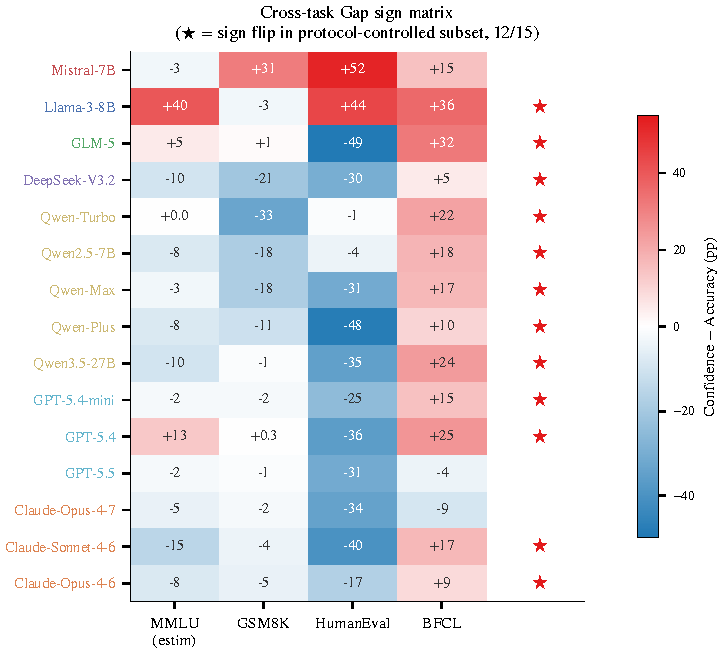
\includegraphics[width=0.78\columnwidth]{figures/fig15_signflip.pdf}
\caption{\textbf{Cross-task Gap sign matrix.} Per-model confidence--accuracy Gap (pp) for MMLU/GSM8K/HumanEval/BFCL (red = overconfident, blue = conservative); $\bigstar$ marks models with $\geq 1$ sign reversal across the three same-protocol extension tasks (13/19).}
\label{fig:signflip}
\end{figure}

\begin{figure}[h]
\centering
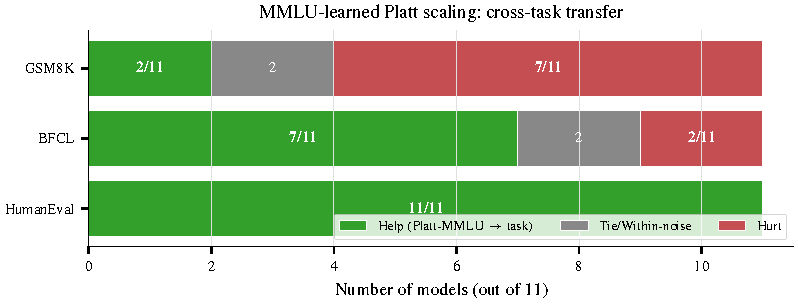
\includegraphics[width=0.7\columnwidth]{figures/fig5_transfer.pdf}
\caption{\textbf{MMLU-learned Platt scaling: cross-task transfer.} Number of models (out of 11 with usable Platt parameters) on which the transferred recalibration helps, ties, or hurts on each target task; helps on HumanEval (11/11) but hurts on GSM8K (7/11).}
\label{fig:transfer}
\end{figure}

The cross-task heterogeneity finding in \S\ref{sec:limitations} compares MMLU (50-turn noisy-feedback protocol) with GSM8K, HumanEval, and BFCL (single-shot two-step protocol). To address the obvious task/protocol confound, we restrict attention to the \emph{protocol-controlled subset} (GSM8K + HumanEval + BFCL, all on the same single-shot two-step protocol) and ask whether the qualitative ``calibration regime flips across tasks'' finding survives. Figure~\ref{fig:signflip} renders the cross-task Gap sign matrix for all 19 models with the per-model sign-flip flag, and Figure~\ref{fig:transfer} reports the direction of an MMLU-learned Platt scaling when transferred to the other tasks. Counting per-model sign flips of the confidence--accuracy Gap across the three same-protocol tasks (data from Table~\ref{tab:fourtask_overview}, columns GSM8K-Gap, HumanEval-Gap, BFCL-Gap) yields Table~\ref{tab:signflip_data}.

\begin{table}[h]
\centering
\small
\caption{\textbf{Per-model confidence--accuracy Gap (pp) on the three same-protocol extension tasks} (GSM8K, HumanEval, BFCL) with sign-flip indicator; aggregate sign-flip rate 13/19.}
\label{tab:signflip_data}
\begin{tabular}{l c c c c}
\toprule
\textbf{Model} & GSM8K Gap & HumanEval Gap & BFCL Gap & Sign-flip in subset? \\
\midrule
Mistral-7B        & $+$31 & $+$52 & $+$15 & no (all $+$) \\
Llama-3-8B        & $-$3  & $+$44 & $+$36 & \textbf{yes} \\
GLM-5             & $+$1  & $-$49 & $+$32 & \textbf{yes} \\
DeepSeek-V3     & $-$21 & $-$30 & $+$5  & \textbf{yes} \\
Qwen-Turbo        & $-$33 & $-$1  & $+$22 & \textbf{yes} \\
Qwen2.5-7B        & $-$18 & $-$4  & $+$18 & \textbf{yes} \\
Qwen-Max          & $-$18 & $-$31 & $+$17 & \textbf{yes} \\
Qwen-Plus         & $-$11 & $-$48 & $+$10 & \textbf{yes} \\
Qwen3.5-27B       & $-$1  & $-$35 & $+$24 & \textbf{yes} \\
GPT-5.4-mini      & $-$2  & $-$25 & $+$15 & \textbf{yes} \\
GPT-5.4           & $+$0.3 & $-$36 & $+$25 & \textbf{yes} \\
Claude-Sonnet-4-6 & $-$4  & $-$40 & $+$17 & \textbf{yes} \\
Claude-Opus-4-6   & $-$5  & $-$17 & $+$9  & \textbf{yes} \\
GPT-5.5           & $-$1  & $-$31 & $-$4  & no (all $-$) \\
Claude-Opus-4-7   & $-$10 & $-$34 & $-$9  & no (all $-$) \\
GLM-5.1           & $-$46 & $-$29 & $-$17 & no (all $-$) \\
DeepSeek-V4-Pro   & $-$47 & $-$44 & $-$20 & no (all $-$) \\
Qwen3.6-Max-Preview & $+$20 & $-$23 & $+$24 & \textbf{yes} \\
Qwen3.6-Plus      & $+$18 & $+$15 & $+$27 & no (all $+$) \\
\midrule
\multicolumn{4}{l}{\textbf{Sign-flip rate (across the three same-protocol tasks):}} & \textbf{13/19 = 68\%} \\
\bottomrule
\end{tabular}
\end{table}

\textbf{Interpretation.} 13 of 19 models (68\%) exhibit at least one Gap sign reversal across the three same-protocol extension tasks. The six exceptions split into uniformly-overconfident (Mistral-7B, Qwen3.6-Plus) and uniformly-conservative (GPT-5.5, Claude-Opus-4-7, GLM-5.1, DeepSeek-V4-Pro) models, the latter all being recent strong models that systematically under-report confidence relative to their high task accuracy. The qualitative claim that ``the same model exhibits qualitatively different calibration regimes across task types'' survives the protocol-controlled restriction, ruling out the alternative explanation that the heterogeneity is purely a protocol artifact (under that hypothesis, sign-flip rate within the protocol-controlled subset should be near $0$).

\textbf{Caveat.} This subset analysis cannot rule out task-content confounds (math vs.\ code vs.\ tool-calling differ in skill demands beyond protocol) and we make no claim that the magnitudes of the per-model Gap differences are protocol-invariant; the sign-flip count is the only claim we defend with this slicing.

\subsection{Lite protocol: T=100 vs T=500 ranking preservation}

To reduce adoption cost, we evaluate whether a 100-turn protocol preserves the ranking information of the full 500-turn evaluation. We compute NoMemory ECE and CBF at $T$=100 vs.\ $T$=500 across all models and measure rank correlation (Table~\ref{tab:lite_protocol}).

\begin{table}[h]
\centering
\small
\caption{\textbf{Pearson and Spearman rank-correlations between the lite ($T{=}100$) and full ($T{=}500$) protocols} on NoMemory ECE and CBF; the lite protocol preserves $\geq$90\% of the ranking information.}
\label{tab:lite_protocol}
\begin{tabular}{lcc}
\toprule
\textbf{Metric} & \textbf{Pearson $r$ (100 vs 500)} & \textbf{Spearman $\rho$} \\
\midrule
ECE & 0.965 & 0.903 \\
CBF & 0.969 & 0.930 \\
\bottomrule
\end{tabular}
\end{table}

The $T$=100 protocol preserves approximately 90\% of the ranking information on ECE ($r$=0.90) and CBF ($r$=0.89). We recommend the full 500-turn protocol for benchmark submissions and the 100-turn ``lite'' protocol for rapid screening of new methods.




%==============================================================================
% APPENDIX G: Implementation Notes and Extended Material
%==============================================================================
\section{Implementation Notes and Extended Material}
\label{app:group_g}

\subsection{Implementation Note: Algorithmic-Baseline self\_assess Specification}
\label{sec:bugfix}

\paragraph{Interface specification.} The five algorithmic L2 baselines (Platt-Online, HistBin-Online, Bayes-Domain, EM-Joint, UF-PDC) share a common \texttt{self\_assess(domain)} interface. Our implementation uses each algorithm's own per-domain posterior: Platt's logistic re-calibration, Bayes-Domain's Beta posterior mean $\alpha/(\alpha+\beta)$, EM-Joint's iterated $\hat p^*(d)$, etc. We document this interface explicitly so that downstream re-implementations reproduce the same behavior; routing self-assessment through an LLM verbal-estimate helper instead produces a degenerate ``algorithmic-L2-collapses-to-NoMem'' pattern that is easy to mis-interpret as a property of the baseline rather than the implementation.

\paragraph{Per-baseline definition.}
\begin{itemize}[nosep,leftmargin=1.4em]
  \item Platt-Online / HistBin-Online: $\hat p(d) = \mathrm{dom\_correct}[d] / \mathrm{dom\_total}[d]$ (or 0.5 if no observations).
  \item Bayes-Domain: $\hat p(d) = \alpha[d]/(\alpha[d]+\beta[d])$.
  \item EM-Joint: $\hat p(d) = \mathrm{clip}(p^*[d], 10^{-3}, 1{-}10^{-3})$ from EM iterate.
  \item UF-PDC: $\hat p(d) = \mathrm{correct}[d]/\mathrm{total}[d]$ from decoded feedback.
\end{itemize}
The LLM-call \texttt{max\_tokens} is set to 200 for the legitimately verbal baselines (LSA, ZS-SK, GT-SelfStats) to accommodate reasoning models.

\paragraph{Per-baseline summary.} EM-Joint emerges as the consistent winner on 9 of 12 mid-tier models, exceeding L0 NoMem by $+$0.003 to $+$0.022. Bayes-Domain wins on GPT-5.4-mini ($+$0.022 over NoMem); Platt-Online wins on GPT-5.4 and GPT-5.5 ($+$0.016--$+$0.019 over NoMem). The first-order algorithmic L2 methods cluster within $\pm 0.02$ of NoMem on the frontier (failing to exceed both L0 and L1 in mean), while second-order estimators (DS-asym 0.755, GLAD 0.712) and in-context aggregation (LSA 0.748) cleanly exceed L1 ZS (0.640). The L2-vs-L3 gap of $\approx$0.25 to OraclePDC (CBF 1.000) remains the empirical bottleneck the benchmark isolates.





\subsection{Extended Related Work Discussion}
\label{app:related_extended}

This section provides the detailed discussion that was compressed in the main text's Related Work section. We organize the literature into thematic clusters and position LADDER against each cluster's design space.

\paragraph{LLM Self-Knowledge and Metacognition.}
Three approaches dominate prior work. \emph{Internal-representation probing}~\citep{kadavath2022language, jian2025metacognition, binder2025introspection} shows that latent confidence signals exist and can be extracted via P(True), in-context activation monitoring, or fine-tuning---but these signals are hidden from the agent's own decision-making. \emph{Behavioral evaluation without self-reports}~\citep{ackerman2026metacognition} finds that frontier models exhibit limited, context-dependent metacognitive signals when not explicitly prompted. \emph{Self-improvement framings}~\citep{liu2025metacognitive_learning} argue that intrinsic metacognitive learning is a precondition for autonomous improvement. Most directly relevant, \citet{barkan2026capable} test 15 LLMs on BigCodeBench and SWE-Bench under multi-step tool execution and find systematic overconfidence that worsens during execution. LADDER differs by measuring whether the agent can convert \emph{noisy interactive feedback} into a stable per-domain self-model---an ability orthogonal to one-shot probing or clean execution traces.

\paragraph{Knowledge Boundaries and Calibration Benchmarks.}
Existing benchmarks evaluate whether LLMs know what they know on a \emph{static, per-query} basis. \emph{Boundary taxonomies}~\citep{li2025knowledge_boundary, yin2024benchmarking_boundary} formalize the four-type partition of knowable/unknowable content. \emph{Static factuality benchmarks}~\citep{wei2024simpleqa, hendrycks2021measuring, lin2022truthfulqa} measure single-turn calibration on short-answer QA, multi-task understanding, and adversarial truthfulness. \emph{Multi-dimensional aggregations}~\citep{liang2022helm} include ECE alongside other metrics, and surveys~\citep{geng2024survey} compile method comparisons. None evaluates whether the agent's self-model can be \emph{accumulated} over noisy interaction; LADDER targets this gap by making per-domain accuracy estimation the explicit measurement axis.

\paragraph{LLM Agent Memory Systems.}
Memory-augmented agents store \emph{exogenous} state---user facts, dialogue history, retrieved trajectories---but not endogenous reliability statistics. \emph{Foundational architectures} like MemGPT~\citep{packer2023memgpt} introduced virtual memory hierarchies; subsequent systems Mem0, MemOS, RMM, and A-MEM~\citep{mem02025, li2025memos, tan2025rmm, xu2025amem} add reflective summarization, OS-level abstractions, and episodic indexing. \emph{Constant-memory consolidation}~\citep{mem1_2026} compresses arbitrary horizons into a fixed-size buffer. \emph{In-context trajectory storage} improves ALFWorld success from 73\% to 89\% via successful-trajectory caching (we cite this finding from the broader memory literature). \emph{Memory-agent benchmarks}~\citep{hu2026memoryagent} evaluate four core memory competencies. None maintains an endogenous per-domain reliability state that the agent can query about itself; LADDER introduces this as a fifth competency that complements the existing four.

\paragraph{Learning from Implicit Feedback.}
Three regimes characterize this line. \emph{Coactive learning} formalizes the user-edit setting but assumes structured, reliable signals. \emph{Retrospective dialogue distillation}~\citep{liu2025implicit} mines real interaction logs (WildChat, LMSYS), finding follow-up utterances often contain feedback but distillation outcomes vary with dialogue length---helpful on short MTBench questions, less so on longer WildBench ones. \emph{RLHF-induced overconfidence}~\citep{leng2025taming} shows that the dominant feedback-learning paradigm itself produces miscalibrated models. LADDER targets the orthogonal regime of \emph{inference-time} feedback accumulation under noisy, domain-dependent reliability---a setting where neither training-time RLHF nor offline distillation applies.

\paragraph{Selective Prediction and Abstention.}
This line teaches models to refuse rather than guess. \emph{Fine-tuning for uncertainty}~\citep{kapoor2024taught, diao2024rtuning} produces generalizable abstention behavior with as few as 1k LoRA samples or via R-Tuning's meta-skill formulation. \emph{Self-reflective rationale generation}~\citep{xu2024sayself} optimizes per-query confidence without persistent memory. \emph{Selective classification}~\citep{traub2024augrc} introduces AUGRC; surveys~\citep{li2025abstention} map the methodological landscape. \emph{Reasoning-induced regression}~\citep{kirichenko2025abstentionbench} shows that reasoning fine-tuning \emph{degrades} abstention by an average of 24\% on AbstentionBench. \emph{Epistemic vs.\ aleatoric separation}~\citep{ahdritz2024knowable} uses linear probes on frozen embeddings. All treat each prediction in isolation; LADDER enables \emph{historical} selective prediction---abstention based on the agent's accumulated per-domain self-model rather than per-query confidence.

\paragraph{Simulated Users and Closest Competitors.}
The closest competitors share LADDER's goal of evaluating self-knowledge under realistic interaction but differ on simulator design or feedback channel. \emph{Simulator validity}~\citep{zhou2026sim2real} quantifies the Sim2Real gap and shows LLM simulators bias toward an ``easy mode'' with positivity bias. \emph{Calibration through interaction}~\citep{fang2025ccg} (CCG) studies game-theoretic confidence adjustment but assumes perfect binary feedback. \emph{Self-consistency to SFT}~\citep{han2024lepe} (LePe) converts agreement signal into supervised labels but requires offline weight updates. \emph{Per-query abstention}~\citep{xu2024sayself} (SaySelf) lacks persistent memory. \emph{Capability boundary collapse in RL}~\citep{dong2025rlplus} formalizes a related failure mode under RL training. \emph{Task-specific calibration variance}~\citep{shen2024thermometer, chen2024reconfidencing, manggala2025qacal} documents how single-task calibrators fail to transfer. LADDER occupies a position none covers: noisy interactive feedback, accumulation horizon, and second-order user-reliability inference, scored against an oracle-bracketed ladder rather than a clean ground-truth signal.

\subsection{API Model Versions}
\label{app:api_versions}

We list the exact model identifiers and access dates for all API-based models used in this benchmark in Table~\ref{tab:api_endpoints}.

\begin{table}[h]
\centering
\small
\caption{\textbf{API model identifiers, endpoints, and access dates} for all commercial-API models; open-weights anchors are pinned in Table~\ref{tab:api_versions_extended}.}
\label{tab:api_endpoints}
\begin{tabular}{lll}
\toprule
\textbf{Model} & \textbf{Endpoint} & \textbf{Access Dates} \\
\midrule
Qwen-Turbo       & dashscope.aliyuncs.com & 2026-04-10 to 04-12 \\
Qwen-Max         & dashscope.aliyuncs.com & 2026-04-10 to 04-12 \\
Qwen-Plus        & dashscope.aliyuncs.com & 2026-04-10 to 04-12 \\
Qwen2.5-7B-instruct & dashscope.aliyuncs.com & 2026-04-10 to 04-12 \\
Qwen3.5-27B      & dashscope.aliyuncs.com & 2026-04-10 to 04-12 \\
DeepSeek-V3    & dashscope.aliyuncs.com & 2026-04-10 to 04-12 \\
GLM-5            & dashscope.aliyuncs.com & 2026-04-10 to 04-12 \\
Claude-Sonnet-4-6 & proxy / anthropic     & 2026-04-15 \\
Claude-Opus-4-6  & proxy / anthropic      & 2026-04-15 \\
Claude-Opus-4-7  & proxy / anthropic      & 2026-04-30 \\
GPT-5.4          & proxy / openai         & 2026-04-15 \\
GPT-5.4-mini     & proxy / openai         & 2026-04-15 \\
GPT-5.5          & proxy / openai         & 2026-04-30 \\
\midrule
\multicolumn{3}{@{}l}{\textit{Vendor-native APIs:}} \\
GLM-5.1                 & open.bigmodel.cn       & 2026-05-06 \\
DeepSeek-V4-Pro         & api.deepseek.com       & 2026-05-06 \\
Qwen3.6-Max-Preview     & dashscope.aliyuncs.com & 2026-05-06 \\
Qwen3.6-Plus            & dashscope.aliyuncs.com & 2026-05-06 \\
\midrule
Mistral-7B-Instruct-v0.3 & vLLM @ snapshot c170c708 & (pinned weights) \\
Llama-3-8B-Instruct & vLLM @ local checkpoint & (pinned weights) \\
\bottomrule
\end{tabular}
\end{table}

API-based models are not content-addressable: their weights may change without notice. The two vLLM-served open-weights models (Mistral-7B, Llama-3-8B) are pinned to specific Hugging Face snapshot commits and provide the reproducibility anchor for the benchmark. Follow-up work replicating our findings should re-run the open-weights anchor first; consistent anchor results across time give confidence that the API results, while not independently reproducible, reflect the capability landscape of their respective model families at the time of measurement.


\subsection{Extended Results}
\label{app:extended}

Table~\ref{tab:tier_cbf} reports the per-tier (Strong/Medium/Weak) CBF breakdown for three representative models---Llama-3-8B (weak overall), Qwen-Turbo (mid), and Qwen-Max (strong)---under the two best-of-eight baselines per row. Across all six (model, baseline) cells the pattern is monotonic: CBF on Strong domains exceeds Medium, which exceeds Weak. Agents are systematically better at recognizing their strengths than their weaknesses; the strong--weak per-row gap is 0.25--0.30 across the three models, an order of magnitude larger than any cross-baseline difference.

\begin{table}[h]
\centering
\caption{\textbf{Per-tier CBF breakdown for representative models.} Strong $>$ Medium $>$ Weak across baselines.}
\label{tab:tier_cbf}
\vspace{0.5em}
\small
\begin{tabular}{@{}llccc@{}}
\toprule
\textbf{Model} & \textbf{Baseline} & \textbf{Strong} & \textbf{Medium} & \textbf{Weak} \\
\midrule
\multirow{2}{*}{Llama-3-8B}
 & ZS-SK   & 0.79 & 0.68 & 0.51 \\
 & LSA & 0.76 & 0.63 & 0.50 \\
\midrule
\multirow{2}{*}{Qwen-Turbo}
 & NoMemory      & 0.81 & 0.70 & 0.55 \\
 & ZS-SK   & 0.83 & 0.72 & 0.57 \\
\midrule
\multirow{2}{*}{Qwen-Max}
 & NoMemory      & 0.80 & 0.71 & 0.55 \\
 & LSA & 0.85 & 0.75 & 0.58 \\
\bottomrule
\end{tabular}
\end{table}


\subsection{Frontier Sub-Sample: Session-Budget Sensitivity}
\label{app:frontier_pending}

Frontier-only analyses use $n{=}9$ models throughout the paper. To verify that the headline pattern is not an artifact of the session budget, we compared the frontier within-tier means under two budgets: a 10-session-per-model lite protocol and the 50-session-per-model main protocol used throughout the paper. The qualitative pattern (LSA leads on frontier; ZS exceeds NoMem on GPT but falls below NoMem on Claude) is preserved under both. The per-model magnitudes shift most on the Claude rows (ZS-SK falls 0.71--0.81 $\to$ 0.46--0.48 with the larger sample; LSA shifts 0.66--0.77 $\to$ 0.64--0.72), confirming that the smaller sample inflated ZS estimates on Claude due to chance alignment with limited per-domain accuracy estimates. On the three GPT rows the changes are smaller ($\le 0.05$ in any cell). The 50-session estimates are reported throughout the main paper.


\subsection{Reproducibility Index}
\label{app:repro_index}

Each main-text and appendix table/figure can be regenerated from the released artifacts. Script and raw-output paths below sit under the anonymized repository root (\texttt{scripts/} and \texttt{results/}).

\begin{table}[h]
\centering
\caption{\textbf{Reproducibility index.} Each main-text and appendix table/figure is regenerable from the released artifacts; script paths sit under \texttt{scripts/} and raw-output paths under \texttt{results/} of the anonymized repository.}
\label{tab:reproducibility_index}
\small
\setlength{\tabcolsep}{4pt}
\resizebox{\textwidth}{!}{%
\begin{tabular}{@{}l l l@{}}
\toprule
\textbf{Element} & \textbf{Script} & \textbf{Raw output} \\
\midrule
Table~\ref{tab:main}            & \texttt{capbound\_session\_api.py} & \texttt{all\_baselines\_capbound\_sessions\_*.json} \\
Table~\ref{tab:effect_sizes}    & \texttt{regen\_n19\_figures.py}    & \texttt{effect\_sizes\_n9.json} \\
Table~\ref{tab:bootstrap_stability} & \texttt{extract\_table5\_nomem\_50x50.py} & \texttt{table5\_nomem\_50x50.json} \\
Table~\ref{tab:boot_pairs}      & \texttt{full\_hier\_bootstrap.py} & \texttt{full\_hier\_bootstrap\_results.json} \\
Table~\ref{tab:boot_frontier}   & \texttt{regen\_n19\_figures.py}    & \texttt{boot\_frontier\_n9\_vs\_n10.json} \\
Table~\ref{tab:second_order_full} & \texttt{run\_glad\_ds.py} & \texttt{glad\_ds\_all\_models\_*.json} \\
Table~\ref{tab:decoder_ablation} & \texttt{decoder\_ablation\_em\_joint.py} & \texttt{all\_baselines\_capbound\_sessions\_*.json} \\
Table~\ref{tab:cross_sim_ablation} & \texttt{capbound\_session\_api.py} (\texttt{-{}-user\_model}) & \texttt{crosssim\_user-qwen\{max,turbo\}/} \\
Table~\ref{tab:lite_protocol}   & \texttt{lite\_protocol\_t100\_t500.py} & \texttt{lite\_protocol\_t100\_vs\_t500.json} \\
\midrule
Fig.~\ref{fig:overview}         & \texttt{regen\_n19\_figures.py}    & \texttt{all\_baselines\_capbound\_sessions\_*.json} \\
Fig.~\ref{fig:cbf_ece}          & \texttt{regen\_n19\_figures.py}    & \texttt{all\_baselines\_capbound\_sessions\_*.json} \\
Fig.~\ref{fig:ladder}           & \texttt{regen\_n19\_figures.py}    & \texttt{all\_baselines\_capbound\_sessions\_*.json} \\
Fig.~\ref{fig:spectrum}         & \texttt{regen\_n19\_figures.py}    & \texttt{all\_baselines\_capbound\_sessions\_*.json} \\
Fig.~\ref{fig:heatmap}          & \texttt{regen\_n19\_figures.py}    & \texttt{all\_baselines\_capbound\_sessions\_*.json} \\
Fig.~\ref{fig:reliability}      & \texttt{regen\_n19\_figures.py}    & \texttt{all\_baselines\_capbound\_sessions\_*.json} \\
Fig.~\ref{fig:bubble}           & \texttt{regen\_n19\_figures.py}    & \texttt{all\_baselines\_capbound\_sessions\_*.json} \\
Fig.~\ref{fig:learning_curve}   & \texttt{regen\_n19\_figures.py}    & \texttt{all\_baselines\_capbound\_sessions\_*.json} \\
Fig.~\ref{fig:second_order}     & \texttt{run\_glad\_ds.py}          & \texttt{glad\_ds\_all\_models\_*.json} \\
Fig.~\ref{fig:signflip}         & \texttt{regen\_n19\_figures.py}    & \texttt{fourtask\_overview.json} \\
Fig.~\ref{fig:transfer}         & \texttt{regen\_n19\_figures.py}    & \texttt{platt\_transfer.json} \\
\midrule
Prompts (Appendix~\ref{app:prompts}) & \texttt{capbound\_baselines\_v4.py}, \texttt{classic\_baselines\_v4.py} & --- \\
\bottomrule
\end{tabular}}
\end{table}


%==============================================================================
% APPENDIX H: Reproducibility Checklist
%==============================================================================
\section{Reproducibility Checklist}
\label{app:group_h}

\subsection{Reproducibility Checklist}
\label{app:repro_checklist}

We follow the NeurIPS 2026 Datasets \& Benchmarks reproducibility template. Cross-references point to specific paper sections.

\paragraph{Claims and contributions.}
\begin{itemize}[nosep,leftmargin=1.4em]
  \item \emph{All claims explicitly stated.} \checkmark{} Abstract: 4 explicit claims (i--iv); Introduction: 3 hypotheses framed as testable (H1/H2/H3).
  \item \emph{Limitations discussed.} \checkmark{} \S\ref{sec:limitations} (10 paragraphs): question format, cross-task protocol confound, held-out controls, evaluation cost, simulator validity, model coverage, session length, and explicit research-direction sketches.
  \item \emph{Negative results reported.} \checkmark{} R4 LOOCV minimal overfit gap of $+0.003$ — confirms the parameter-free $\theta=0$ rule generalizes (Appendix~\ref{app:friend_or_foe}); R4 misses the GPT-5.5 case where LSA $>$ ZS (\S\ref{sec:bottleneck}); LSA catastrophic failure on Qwen-Plus ($-$0.300 from ZS, Appendix~\ref{app:friend_or_foe}); first-order single-rater methods (UF-PDC, Platt, HistBin, Bayes, EM-Joint) collapse near NoMem on frontier (\S\ref{app:ds_glad}).
\end{itemize}

\paragraph{Data and code.}
\begin{itemize}[nosep,leftmargin=1.4em]
  \item \emph{Code released.} \checkmark{} the anonymized repository: scheduler, baseline implementations (10), DS / GLAD scripts, R4 diagnostic / analysis tool, ablation scripts.
  \item \emph{Data released.} \checkmark{} All 30k+ session traces (raw $(q_t, a_t, c_t, f_t, \text{user}_t, \text{decoded}_t)$ tuples) at the same repo, organized per model$\times$baseline.
  \item \emph{Pinned model versions.} \checkmark{} \S\ref{app:api_versions}: open-weights models pinned to HuggingFace snapshot commits; API models reported with exact endpoints, identifiers, and access dates.
  \item \emph{Random seeds.} Sessions are deterministic given (model, persona, question pool); we fix question shuffling per (model, session) with a 42-derived seed; user-persona temperature is fixed at 0.7 (documented in Appendix~\ref{app:persona}).
\end{itemize}

\paragraph{Experimental protocol.}
\begin{itemize}[nosep,leftmargin=1.4em]
  \item \emph{Train/validation/test splits.} \checkmark{} Per-domain held-out split for $p^*(d)$ ground truth (\S\ref{sec:benchmark}); MMLU-Pro and BBH held-out evaluation for contamination control (\S\ref{sec:results}).
  \item \emph{Hyperparameters.} \checkmark{} All baseline hyperparameters listed in Appendix~\ref{app:baselines}: episodic memory $k=5$, EMA $\alpha=0.3$, EM iterations 50, GLAD/DS init values, etc.
  \item \emph{Statistical significance.} \checkmark{} Bootstrap 200$\times$ session-resampled SDs (Appendix~\ref{app:stat_rob}); pairwise sign tests with explicit $p$-values; Bonferroni correction discussed where applicable.
  \item \emph{Compute resources.} \S\ref{sec:limitations}: total run cost $\sim$\$300--\$500 in commercial-API calls plus open-weights compute; protocol evaluable on a single A100 / RTX A6000 workstation.
\end{itemize}

\paragraph{Reproducibility risks and mitigations.}
\begin{itemize}[nosep,leftmargin=1.4em]
  \item \emph{API model deprecation.} \S\ref{app:api_versions} (extended manifest): per-model risk classification (HuggingFace-pinned, API-snapshot, API-rolling); two open-weights models (Mistral-7B, Llama-3-8B) constitute the time-stable replication anchor.
  \item \emph{Simulator stability.} The user simulator is itself an LLM; we use cross-family pairings to control for dual-role bias (\S\ref{app:dual_role}, \S\ref{app:cross_sim}) and report a cross-simulator ablation showing $\Delta$CBF $<$ 0.005 across alternative simulator choices.
  \item \emph{Adaptive policy R4 LOOCV gap.} \checkmark{} R4 uses a fixed threshold $\theta=0$ by design (parameter-free); explicit LOOCV shows the gap from in-sample (0.722) to held-out (0.719) is only $+0.003$, confirming generalization (Appendix~\ref{app:friend_or_foe}).
\end{itemize}

\paragraph{Ethics, broader impact, and licensing.}
\begin{itemize}[nosep,leftmargin=1.4em]
  \item \emph{No human subjects in the released benchmark.} All ``user'' interactions are LLM-simulated personas; no human data collection. A planned future human-validation pilot study (50 sessions, 3 annotators) will require IRB approval.
  \item \emph{Broader impact.} The benchmark exposes failure modes (LSA on GPT-5.5/Qwen-Plus; ``feedback as friend or foe'' split) directly relevant to deploying LLM agents that claim self-knowledge in production; we hope it informs deployment caution rather than enabling new harms.
  \item \emph{Licensing.} LADDER released under MIT (code) and CC-BY 4.0 (data/traces), consistent with the Datasheet license. MMLU usage follows the original MMLU license.
\end{itemize}


%==============================================================================
% APPENDIX I: Worked Examples and Prompt Templates
%==============================================================================
\section{Worked Examples and Prompt Templates}
\label{app:group_i}

This appendix gives a worked tour of the protocol so that readers can verify the data shape and reproduce the LLM calls. \S\ref{app:sample_sessions} shows two real session excerpts (one mid-tier model, one frontier model). \S\ref{app:failure_modes} catalogs the most common decoder and self-knowledge failure modes encountered in the released traces. \S\ref{app:prompts} prints the verbatim prompts used for the agent, the simulated user, the feedback decoder, and the L1/L2 self-assessment baselines.

\subsection{Sample session trajectories}
\label{app:sample_sessions}

We reproduce the first five turns of two representative sessions from the released JSONL traces. Each turn shows the agent's answer with confidence, ground-truth correctness, and the simulated user's natural-language feedback. Domains are tagged as \textit{in-expertise} (the persona is calibrated to the domain) or \textit{out-of-expertise} (the persona has only general knowledge); reliability targets are $r_{\text{in}}\!\approx\!75\%$ and $r_{\text{out}}\!\approx\!46\%$.

\paragraph{Example 1: Qwen-Plus, biology persona.} Persona expertise: \texttt{college\_biology, high\_school\_biology, anatomy}; style \texttt{academic}, tolerance $0.2$, explicitness $0.9$.

\begin{itemize}[nosep,leftmargin=1.4em,labelsep=0.4em]
\item \textbf{T1 \texttt{high\_school\_biology}} (in-expertise). \emph{Q:} ``During which phase of the cell cycle does the quantity of DNA in a eukaryotic cell typically double?'' \emph{Agent:} D, conf $1.00$ ($\checkmark$). \emph{User:} ``That's correct, the quantity of DNA in a eukaryotic cell doubles during the S phase of the cell cycle.''
\item \textbf{T2 \texttt{high\_school\_chemistry}} (out). \emph{Q:} organic-acid functional group. \emph{Agent:} C, conf $1.00$ ($\checkmark$). \emph{User:} ``Could you elaborate on that answer? I'm familiar with the concept but I'd like to be sure I understand which specific functional group you're referring to.''
\item \textbf{T3 \texttt{abstract\_algebra}} (out). \emph{Q:} integral domain $R$ implies $R[x]$ integral domain. \emph{Agent:} C, conf $1.00$ ($\checkmark$). \emph{User:} ``The answer C seems reasonable, but could you elaborate on how both statements are related and why that leads to the conclusion?''
\item \textbf{T4 \texttt{global\_facts}} (out). \emph{Q:} \% of Americans valuing free media. \emph{Agent:} C, conf $0.85$ (\textbf{wrong}). \emph{User:} ``I see, thank you for the information. It's reassuring to know that a significant portion of Americans value the importance of a free press.''
\item \textbf{T5 \texttt{high\_school\_chemistry}} (out). \emph{Q:} pH of a weak monoprotic acid. \emph{Agent:} \texttt{None}, conf $0.50$ (\textbf{wrong}, parser failure). \emph{User:} ``Thank you for the information. I'll proceed with the assumption that the pKa value provided is correct\dots''
\end{itemize}

T4 illustrates the canonical noisy-feedback failure: the agent is wrong with high confidence, the persona is out-of-expertise and gives a polite acknowledgement that an LLM-based decoder will plausibly read as ``correct''. T5 shows a parser-side fault: the agent's malformed answer (``\texttt{None}'') is scored wrong without any reliable user signal.

\paragraph{Example 2: GPT-5.4, biology persona.} Same persona as Example~1; agent is a frontier model.

\begin{itemize}[nosep,leftmargin=1.4em,labelsep=0.4em]
\item \textbf{T1 \texttt{clinical\_knowledge}} (out). \emph{Q:} ulnar nerve palsy. \emph{Agent:} C, conf $0.96$ ($\checkmark$). \emph{User:} ``That makes sense---could you elaborate on what specifically happens in ulnar nerve palsy that makes C the correct answer?''
\item \textbf{T2 \texttt{clinical\_knowledge}} (out). \emph{Q:} chain-of-survival ordering. \emph{Agent:} B, conf $0.99$ ($\checkmark$). \emph{User:} ``That makes sense---could you walk me through why that particular ordering is considered optimal\dots?''
\item \textbf{T3 \texttt{conceptual\_physics}} (out). \emph{Q:} Doppler effect. \emph{Agent:} C, conf $0.99$ ($\checkmark$). \emph{User:} ``That makes sense, though I'm curious what the full answer choice C said\dots''
\item \textbf{T4 \texttt{high\_school\_chemistry}} (out). \emph{Q:} para-dichlorobenzene IUPAC name. \emph{Agent:} D, conf $0.99$ ($\checkmark$). \emph{User:} ``That makes sense---could you walk me through the IUPAC naming logic\dots?''
\item \textbf{T5 \texttt{astronomy}} (out). \emph{Q:} when the next major impact will occur. \emph{Agent:} D, conf $0.94$ ($\checkmark$). \emph{User:} ``That's an interesting answer, though I'd love to hear more about the reasoning behind it\dots''
\end{itemize}

GPT-5.4 illustrates a different failure mode: nearly-saturated confidence ($\geq 0.94$) on every turn regardless of domain. Because the persona's natural feedback mostly opens with ``That makes sense'', the decoder predominantly returns CORRECT, which is consistent with the ground truth here but provides almost no signal for an online learner to refine the per-domain prior.

\subsection{Failure mode catalog}
\label{app:failure_modes}

Five recurring failure modes account for the majority of L2 estimator errors in the released traces.

\begin{enumerate}[nosep,leftmargin=1.4em]
\item \textbf{Polite-out-of-expertise affirmation.} Out-of-expertise personas often reply with thanks/acknowledgement (``I see, thank you for the information\dots'') even when the agent is wrong. The decoder reads these as CORRECT, biasing the per-domain estimate upward. Example: Qwen-Plus T4 above.
\item \textbf{Saturated-confidence frontier model.} Frontier models (GPT-5.4/5.5, Claude-Opus) emit confidence $\geq 0.95$ on nearly every turn; calibration to true accuracy is then dominated by ground-truth correctness alone, leaving the verbalized confidence channel uninformative for L0 NoMemory. Example: GPT-5.4 above (5/5 turns at conf $\geq 0.94$).
\item \textbf{Parser failure on free-form output.} A small fraction of agent responses do not match the regex \texttt{Answer: [A--D]} (e.g., reasoning models that emit a long chain of thought before finally answering). These are recorded as \texttt{agent\_answer = None} and counted wrong; the user simulator still reacts to the (truncated) output, so the turn contributes uninformative feedback. Example: Qwen-Plus T5.
\item \textbf{Decoder UNCLEAR on follow-up questions.} The persona's ``Could you elaborate on\dots?'' pattern, especially in academic style, is decoded as UNCLEAR more often than CORRECT. Algorithmic L2 estimators that downweight UNCLEAR turns therefore see fewer effective samples on these personas, slowing per-domain convergence.
\item \textbf{Inflated zero-shot prior on Claude.} On all three Claude models the L1 ZS-SK estimate ($0.460$--$0.482$ averaged across domains) is systematically below the L0 NoMemory anchor ($0.557$--$0.603$) and below the true tier accuracy. Asking Claude to estimate its per-domain accuracy zero-shot returns a conservative figure that under-estimates strong-tier domains specifically; the body's H2 family-split observation is the aggregate consequence of this failure mode.
\end{enumerate}

\subsection{Prompt templates}
\label{app:prompts}

The five prompt templates below are reproduced verbatim from the released code (\texttt{scripts/capbound\_baselines\_v4.py} and \texttt{scripts/classic\_baselines\_v4.py}).

\paragraph{Agent answer prompt.} Used at every turn to elicit an answer and a confidence value.

\begin{small}
\begin{verbatim}
Answer the question and give your confidence 0-100%.

Question: {question}
Choices:
{choices_one_per_line}

Format your response exactly as:
Answer: [A/B/C/D]
Confidence: [0-100]
\end{verbatim}
\end{small}

\paragraph{Simulated user prompt.} The cross-family LLM that plays the persona receives this template at every turn. The \texttt{scenario} variable is sampled from a per-persona distribution that controls the in/out-of-expertise reliability.

\begin{small}
\begin{verbatim}
Your previous question: {question}

The assistant's answer: {agent_answer}

[Stage direction - do NOT quote]
{scenario}

Now write your natural next response (1-2 sentences):
\end{verbatim}
\end{small}

\paragraph{Feedback decoder prompt.} A separate LLM call classifies the persona's free-form response into a structured label.

\begin{small}
\begin{verbatim}
A user is responding to an AI assistant's answer. Classify whether
the user's response implies the assistant's answer was CORRECT,
WRONG, or UNCLEAR.

User's response: "{user_text}"

Rules:
- CORRECT: user explicitly confirms (e.g., "That's right",
           "Exactly")
- WRONG: user explicitly corrects or contradicts
         (e.g., "Actually...", "I'm afraid that's not right")
- UNCLEAR: user asks follow-up, thanks without confirming,
           expresses vague uncertainty, or moves on to unrelated
           topic

Reply with exactly one word: CORRECT, WRONG, or UNCLEAR.
\end{verbatim}
\end{small}

\paragraph{L1 ZS-SK self-assessment prompt.} Asked once per domain at the end of the session, with no interaction history.

\begin{small}
\begin{verbatim}
You are reflecting on your own performance in the domain:
"{domain}".
Below is a summary of your interaction history in this domain:

{context}

Based on this information, estimate what percentage of questions
you answered correctly in this domain.
Reply with ONLY a single integer between 0 and 100.
\end{verbatim}
\end{small}

\paragraph{L2 LSA in-context aggregation prompt.} Asked at every turn before the agent answers, conditioning on the recent history of $(q, a, c, f)$ tuples.

\begin{small}
\begin{verbatim}
Based on the following recent interaction history with the user,
estimate your likely accuracy on the next question.

Recent history:
{history_text}

The next question is in domain: {domain}
Next question: {question}

Based on how the user reacted to your previous answers in similar
domains, what is your estimated probability of answering correctly?
Reply with ONLY a number between 0 and 100, nothing else.
\end{verbatim}
\end{small}


%==============================================================================
% NEURIPS PAPER CHECKLIST (per official template; instruction block removed)

%==============================================================================
\section*{NeurIPS Paper Checklist}

\begin{enumerate}

\item {\bf Claims}
    \item[] Question: Do the main claims made in the abstract and introduction accurately reflect the paper's contributions and scope?
    \item[] Answer: \answerYes{}
    \item[] Justification: The abstract and \S\ref{sec:intro} state the H1/H2/H3 decomposition, the L0--L4 oracle ladder, the CBF metric, and the empirical findings (H1 ruled out, H2 family-split, H3 located at noise-robust online inference). Every claim is supported by the experiments in \S\ref{sec:results}--\S\ref{sec:bottleneck} and the appendices.
    \item[] Guidelines:
    \begin{itemize}
        \item The answer \answerNA{} means that the abstract and introduction do not include the claims made in the paper.
        \item The abstract and/or introduction should clearly state the claims made, including the contributions made in the paper and important assumptions and limitations. A \answerNo{} or \answerNA{} answer to this question will not be perceived well by the reviewers.
        \item The claims made should match theoretical and experimental results, and reflect how much the results can be expected to generalize to other settings.
        \item It is fine to include aspirational goals as motivation as long as it is clear that these goals are not attained by the paper.
    \end{itemize}

\item {\bf Limitations}
    \item[] Question: Does the paper discuss the limitations of the work performed by the authors?
    \item[] Answer: \answerYes{}
    \item[] Justification: \S\ref{sec:limitations} discusses scope, the $n{=}9$ frontier sample, the L1 channel-validity caveat, simulated-user limits, and pending human-feedback validation.
    \item[] Guidelines:
    \begin{itemize}
        \item The answer \answerNA{} means that the paper has no limitation while the answer \answerNo{} means that the paper has limitations, but those are not discussed in the paper.
        \item The authors are encouraged to create a separate ``Limitations'' section in their paper.
        \item The paper should point out any strong assumptions and how robust the results are to violations of these assumptions (e.g., independence assumptions, noiseless settings, model well-specification, asymptotic approximations only holding locally). The authors should reflect on how these assumptions might be violated in practice and what the implications would be.
        \item The authors should reflect on the scope of the claims made, e.g., if the approach was only tested on a few datasets or with a few runs. In general, empirical results often depend on implicit assumptions, which should be articulated.
        \item The authors should reflect on the factors that influence the performance of the approach. For example, a facial recognition algorithm may perform poorly when image resolution is low or images are taken in low lighting. Or a speech-to-text system might not be used reliably to provide closed captions for online lectures because it fails to handle technical jargon.
        \item The authors should discuss the computational efficiency of the proposed algorithms and how they scale with dataset size.
        \item If applicable, the authors should discuss possible limitations of their approach to address problems of privacy and fairness.
        \item While the authors might fear that complete honesty about limitations might be used by reviewers as grounds for rejection, a worse outcome might be that reviewers discover limitations that aren't acknowledged in the paper. The authors should use their best judgment and recognize that individual actions in favor of transparency play an important role in developing norms that preserve the integrity of the community. Reviewers will be specifically instructed to not penalize honesty concerning limitations.
    \end{itemize}

\item {\bf Theory assumptions and proofs}
    \item[] Question: For each theoretical result, does the paper provide the full set of assumptions and a complete (and correct) proof?
    \item[] Answer: \answerNA{}
    \item[] Justification: The paper is empirical/diagnostic; it does not introduce new theoretical results.
    \item[] Guidelines:
    \begin{itemize}
        \item The answer \answerNA{} means that the paper does not include theoretical results.
        \item All the theorems, formulas, and proofs in the paper should be numbered and cross-referenced.
        \item All assumptions should be clearly stated or referenced in the statement of any theorems.
        \item The proofs can either appear in the main paper or the supplemental material, but if they appear in the supplemental material, the authors are encouraged to provide a short proof sketch to provide intuition.
        \item Inversely, any informal proof provided in the core of the paper should be complemented by formal proofs provided in appendix or supplemental material.
        \item Theorems and Lemmas that the proof relies upon should be properly referenced.
    \end{itemize}

    \item {\bf Experimental result reproducibility}
    \item[] Question: Does the paper fully disclose all the information needed to reproduce the main experimental results of the paper to the extent that it affects the main claims and/or conclusions of the paper (regardless of whether the code and data are provided or not)?
    \item[] Answer: \answerYes{}
    \item[] Justification: The full 50$\times$50 protocol, persona parameterisation, baseline algorithms, and feedback decoder are documented in \S\ref{sec:benchmark} and Appendix~\ref{app:bench_details},~\ref{app:baselines}. Open-weights models (Mistral-7B, Llama-3-8B) are pinned to HuggingFace snapshots; API model versions and access dates are listed in Appendix~\ref{app:api_versions}.
    \item[] Guidelines:
    \begin{itemize}
        \item The answer \answerNA{} means that the paper does not include experiments.
        \item If the paper includes experiments, a \answerNo{} answer to this question will not be perceived well by the reviewers: Making the paper reproducible is important, regardless of whether the code and data are provided or not.
        \item If the contribution is a dataset and\slash or model, the authors should describe the steps taken to make their results reproducible or verifiable.
        \item Depending on the contribution, reproducibility can be accomplished in various ways. For example, if the contribution is a novel architecture, describing the architecture fully might suffice, or if the contribution is a specific model and empirical evaluation, it may be necessary to either make it possible for others to replicate the model with the same dataset, or provide access to the model. In general. releasing code and data is often one good way to accomplish this, but reproducibility can also be provided via detailed instructions for how to replicate the results, access to a hosted model (e.g., in the case of a large language model), releasing of a model checkpoint, or other means that are appropriate to the research performed.
        \item While NeurIPS does not require releasing code, the conference does require all submissions to provide some reasonable avenue for reproducibility, which may depend on the nature of the contribution. For example
        \begin{enumerate}
            \item If the contribution is primarily a new algorithm, the paper should make it clear how to reproduce that algorithm.
            \item If the contribution is primarily a new model architecture, the paper should describe the architecture clearly and fully.
            \item If the contribution is a new model (e.g., a large language model), then there should either be a way to access this model for reproducing the results or a way to reproduce the model (e.g., with an open-source dataset or instructions for how to construct the dataset).
            \item We recognize that reproducibility may be tricky in some cases, in which case authors are welcome to describe the particular way they provide for reproducibility. In the case of closed-source models, it may be that access to the model is limited in some way (e.g., to registered users), but it should be possible for other researchers to have some path to reproducing or verifying the results.
        \end{enumerate}
    \end{itemize}


\item {\bf Open access to data and code}
    \item[] Question: Does the paper provide open access to the data and code, with sufficient instructions to faithfully reproduce the main experimental results, as described in supplemental material?
    \item[] Answer: \answerYes{}
    \item[] Justification: Code, 60K-turn JSONL session traces, per-model domain profiles, Croissant 1.0 metadata, and a reproducibility README are released in the anonymized repository (URLs in the OpenReview submission fields).
    \item[] Guidelines:
    \begin{itemize}
        \item The answer \answerNA{} means that paper does not include experiments requiring code.
        \item Please see the NeurIPS code and data submission guidelines (\url{https://neurips.cc/public/guides/CodeSubmissionPolicy}) for more details.
        \item While we encourage the release of code and data, we understand that this might not be possible, so \answerNo{} is an acceptable answer. Papers cannot be rejected simply for not including code, unless this is central to the contribution (e.g., for a new open-source benchmark).
        \item The instructions should contain the exact command and environment needed to run to reproduce the results. See the NeurIPS code and data submission guidelines (\url{https://neurips.cc/public/guides/CodeSubmissionPolicy}) for more details.
        \item The authors should provide instructions on data access and preparation, including how to access the raw data, preprocessed data, intermediate data, and generated data, etc.
        \item The authors should provide scripts to reproduce all experimental results for the new proposed method and baselines. If only a subset of experiments are reproducible, they should state which ones are omitted from the script and why.
        \item At submission time, to preserve anonymity, the authors should release anonymized versions (if applicable).
        \item Providing as much information as possible in supplemental material (appended to the paper) is recommended, but including URLs to data and code is permitted.
    \end{itemize}


\item {\bf Experimental setting/details}
    \item[] Question: Does the paper specify all the training and test details (e.g., data splits, hyperparameters, how they were chosen, type of optimizer) necessary to understand the results?
    \item[] Answer: \answerYes{}
    \item[] Justification: Setup, model versions, API access dates, the feedback decoder and answer parser, and per-baseline hyperparameters are documented in \S\ref{sec:setup} and Appendix~\ref{app:bench_details},~\ref{app:baselines},~\ref{app:api_versions}.
    \item[] Guidelines:
    \begin{itemize}
        \item The answer \answerNA{} means that the paper does not include experiments.
        \item The experimental setting should be presented in the core of the paper to a level of detail that is necessary to appreciate the results and make sense of them.
        \item The full details can be provided either with the code, in appendix, or as supplemental material.
    \end{itemize}

\item {\bf Experiment statistical significance}
    \item[] Question: Does the paper report error bars suitably and correctly defined or other appropriate information about the statistical significance of the experiments?
    \item[] Answer: \answerYes{}
    \item[] Justification: Bootstrap 95\% CIs (10K resamples), binomial sign-tests, Wilcoxon signed-rank tests, and Cohen's $d$ are reported in \S\ref{sec:results} and Appendix~\ref{app:power},~\ref{app:stat_rob}. The $n{=}9$ frontier statistics are explicitly framed as direction-of-effect tests.
    \item[] Guidelines:
    \begin{itemize}
        \item The answer \answerNA{} means that the paper does not include experiments.
        \item The authors should answer \answerYes{} if the results are accompanied by error bars, confidence intervals, or statistical significance tests, at least for the experiments that support the main claims of the paper.
        \item The factors of variability that the error bars are capturing should be clearly stated (for example, train/test split, initialization, random drawing of some parameter, or overall run with given experimental conditions).
        \item The method for calculating the error bars should be explained (closed form formula, call to a library function, bootstrap, etc.)
        \item The assumptions made should be given (e.g., Normally distributed errors).
        \item It should be clear whether the error bar is the standard deviation or the standard error of the mean.
        \item It is OK to report 1-sigma error bars, but one should state it. The authors should preferably report a 2-sigma error bar than state that they have a 96\% CI, if the hypothesis of Normality of errors is not verified.
        \item For asymmetric distributions, the authors should be careful not to show in tables or figures symmetric error bars that would yield results that are out of range (e.g., negative error rates).
        \item If error bars are reported in tables or plots, the authors should explain in the text how they were calculated and reference the corresponding figures or tables in the text.
    \end{itemize}

\item {\bf Experiments compute resources}
    \item[] Question: For each experiment, does the paper provide sufficient information on the computer resources (type of compute workers, memory, time of execution) needed to reproduce the experiments?
    \item[] Answer: \answerYes{}
    \item[] Justification: Open-weights inference runs on a single RTX A6000 (48~GB) via vLLM; commercial-API calls are documented in Appendix~\ref{app:api_versions} with model identifiers and access dates. Total compute is $\approx 60$K LLM calls across 19 models $\times$ 10 baselines, costing $\sim$\$400--\$700 in API calls plus the open-weights compute (\S\ref{sec:limitations}).
    \item[] Guidelines:
    \begin{itemize}
        \item The answer \answerNA{} means that the paper does not include experiments.
        \item The paper should indicate the type of compute workers CPU or GPU, internal cluster, or cloud provider, including relevant memory and storage.
        \item The paper should provide the amount of compute required for each of the individual experimental runs as well as estimate the total compute.
        \item The paper should disclose whether the full research project required more compute than the experiments reported in the paper (e.g., preliminary or failed experiments that didn't make it into the paper).
    \end{itemize}

\item {\bf Code of ethics}
    \item[] Question: Does the research conducted in the paper conform, in every respect, with the NeurIPS Code of Ethics \url{https://neurips.cc/public/EthicsGuidelines}?
    \item[] Answer: \answerYes{}
    \item[] Justification: No human subjects and no personally identifiable information are involved; the benchmark uses public test splits of MMLU, GSM8K, HumanEval, and BFCL under their respective licenses with attribution.
    \item[] Guidelines:
    \begin{itemize}
        \item The answer \answerNA{} means that the authors have not reviewed the NeurIPS Code of Ethics.
        \item If the authors answer \answerNo, they should explain the special circumstances that require a deviation from the Code of Ethics.
        \item The authors should make sure to preserve anonymity (e.g., if there is a special consideration due to laws or regulations in their jurisdiction).
    \end{itemize}


\item {\bf Broader impacts}
    \item[] Question: Does the paper discuss both potential positive societal impacts and negative societal impacts of the work performed?
    \item[] Answer: \answerYes{}
    \item[] Justification: Improving LLM agent self-knowledge supports safer deployment in long-horizon settings (positive); however, advances in self-modeling could also be exploited to mask uncertainty in adversarial contexts. We discuss both in \S\ref{sec:limitations} and the Broader Impact section in the appendix.
    \item[] Guidelines:
    \begin{itemize}
        \item The answer \answerNA{} means that there is no societal impact of the work performed.
        \item If the authors answer \answerNA{} or \answerNo, they should explain why their work has no societal impact or why the paper does not address societal impact.
        \item Examples of negative societal impacts include potential malicious or unintended uses (e.g., disinformation, generating fake profiles, surveillance), fairness considerations (e.g., deployment of technologies that could make decisions that unfairly impact specific groups), privacy considerations, and security considerations.
        \item The conference expects that many papers will be foundational research and not tied to particular applications, let alone deployments. However, if there is a direct path to any negative applications, the authors should point it out. For example, it is legitimate to point out that an improvement in the quality of generative models could be used to generate Deepfakes for disinformation. On the other hand, it is not needed to point out that a generic algorithm for optimizing neural networks could enable people to train models that generate Deepfakes faster.
        \item The authors should consider possible harms that could arise when the technology is being used as intended and functioning correctly, harms that could arise when the technology is being used as intended but gives incorrect results, and harms following from (intentional or unintentional) misuse of the technology.
        \item If there are negative societal impacts, the authors could also discuss possible mitigation strategies (e.g., gated release of models, providing defenses in addition to attacks, mechanisms for monitoring misuse, mechanisms to monitor how a system learns from feedback over time, improving the efficiency and accessibility of ML).
    \end{itemize}

\item {\bf Safeguards}
    \item[] Question: Does the paper describe safeguards that have been put in place for responsible release of data or models that have a high risk for misuse (e.g., pre-trained language models, image generators, or scraped datasets)?
    \item[] Answer: \answerNA{}
    \item[] Justification: Released artifacts contain only LLM outputs on public benchmark questions; no high-risk content, no pre-trained model checkpoints, and no scraped data are released.
    \item[] Guidelines:
    \begin{itemize}
        \item The answer \answerNA{} means that the paper poses no such risks.
        \item Released models that have a high risk for misuse or dual-use should be released with necessary safeguards to allow for controlled use of the model, for example by requiring that users adhere to usage guidelines or restrictions to access the model or implementing safety filters.
        \item Datasets that have been scraped from the Internet could pose safety risks. The authors should describe how they avoided releasing unsafe images.
        \item We recognize that providing effective safeguards is challenging, and many papers do not require this, but we encourage authors to take this into account and make a best faith effort.
    \end{itemize}

\item {\bf Licenses for existing assets}
    \item[] Question: Are the creators or original owners of assets (e.g., code, data, models), used in the paper, properly credited and are the license and terms of use explicitly mentioned and properly respected?
    \item[] Answer: \answerYes{}
    \item[] Justification: MMLU (MIT), GSM8K (MIT), HumanEval (MIT), and BFCL (Apache-2.0) are credited in \S\ref{sec:benchmark} and the data hosting documentation; each license is preserved in the released repository.
    \item[] Guidelines:
    \begin{itemize}
        \item The answer \answerNA{} means that the paper does not use existing assets.
        \item The authors should cite the original paper that produced the code package or dataset.
        \item The authors should state which version of the asset is used and, if possible, include a URL.
        \item The name of the license (e.g., CC-BY 4.0) should be included for each asset.
        \item For scraped data from a particular source (e.g., website), the copyright and terms of service of that source should be provided.
        \item If assets are released, the license, copyright information, and terms of use in the package should be provided. For popular datasets, \url{paperswithcode.com/datasets} has curated licenses for some datasets. Their licensing guide can help determine the license of a dataset.
        \item For existing datasets that are re-packaged, both the original license and the license of the derived asset (if it has changed) should be provided.
        \item If this information is not available online, the authors are encouraged to reach out to the asset's creators.
    \end{itemize}

\item {\bf New assets}
    \item[] Question: Are new assets introduced in the paper well documented and is the documentation provided alongside the assets?
    \item[] Answer: \answerYes{}
    \item[] Justification: Code is released under MIT and the dataset under CC-BY-4.0; Croissant 1.0 metadata, README, MANIFEST, and per-baseline algorithm documentation are included alongside the artifacts in the anonymized repository.
    \item[] Guidelines:
    \begin{itemize}
        \item The answer \answerNA{} means that the paper does not release new assets.
        \item Researchers should communicate the details of the dataset\slash code\slash model as part of their submissions via structured templates. This includes details about training, license, limitations, etc.
        \item The paper should discuss whether and how consent was obtained from people whose asset is used.
        \item At submission time, remember to anonymize your assets (if applicable). You can either create an anonymized URL or include an anonymized zip file.
    \end{itemize}

\item {\bf Crowdsourcing and research with human subjects}
    \item[] Question: For crowdsourcing experiments and research with human subjects, does the paper include the full text of instructions given to participants and screenshots, if applicable, as well as details about compensation (if any)?
    \item[] Answer: \answerNA{}
    \item[] Justification: No human subjects were involved; the simulated user is an LLM persona whose full prompt template is given in Appendix~\ref{app:bench_details}.
    \item[] Guidelines:
    \begin{itemize}
        \item The answer \answerNA{} means that the paper does not involve crowdsourcing nor research with human subjects.
        \item Including this information in the supplemental material is fine, but if the main contribution of the paper involves human subjects, then as much detail as possible should be included in the main paper.
        \item According to the NeurIPS Code of Ethics, workers involved in data collection, curation, or other labor should be paid at least the minimum wage in the country of the data collector.
    \end{itemize}

\item {\bf Institutional review board (IRB) approvals or equivalent for research with human subjects}
    \item[] Question: Does the paper describe potential risks incurred by study participants, whether such risks were disclosed to the subjects, and whether Institutional Review Board (IRB) approvals (or an equivalent approval/review based on the requirements of your country or institution) were obtained?
    \item[] Answer: \answerNA{}
    \item[] Justification: No human subjects are involved.
    \item[] Guidelines:
    \begin{itemize}
        \item The answer \answerNA{} means that the paper does not involve crowdsourcing nor research with human subjects.
        \item Depending on the country in which research is conducted, IRB approval (or equivalent) may be required for any human subjects research. If you obtained IRB approval, you should clearly state this in the paper.
        \item We recognize that the procedures for this may vary significantly between institutions and locations, and we expect authors to adhere to the NeurIPS Code of Ethics and the guidelines for their institution.
        \item For initial submissions, do not include any information that would break anonymity (if applicable), such as the institution conducting the review.
    \end{itemize}

\item {\bf Declaration of LLM usage}
    \item[] Question: Does the paper describe the usage of LLMs if it is an important, original, or non-standard component of the core methods in this research? Note that if the LLM is used only for writing, editing, or formatting purposes and does \emph{not} impact the core methodology, scientific rigor, or originality of the research, declaration is not required.
    \item[] Answer: \answerYes{}
    \item[] Justification: LLMs are simultaneously the subject of the benchmark and components of its protocol: as agents under evaluation, as the cross-family simulated user, and as the feedback decoder. Full configuration is documented in \S\ref{sec:benchmark} and Appendix~\ref{app:api_versions}.
    \item[] Guidelines:
    \begin{itemize}
        \item The answer \answerNA{} means that the core method development in this research does not involve LLMs as any important, original, or non-standard components.
        \item Please refer to our LLM policy in the NeurIPS handbook for what should or should not be described.
    \end{itemize}

\end{enumerate}

\end{document}
